\documentclass{article}\usepackage[]{graphicx}\usepackage[]{color}
%% maxwidth is the original width if it is less than linewidth
%% otherwise use linewidth (to make sure the graphics do not exceed the margin)
\makeatletter
\def\maxwidth{ %
  \ifdim\Gin@nat@width>\linewidth
    \linewidth
  \else
    \Gin@nat@width
  \fi
}
\makeatother

\definecolor{fgcolor}{rgb}{0.345, 0.345, 0.345}
\newcommand{\hlnum}[1]{\textcolor[rgb]{0.686,0.059,0.569}{#1}}%
\newcommand{\hlstr}[1]{\textcolor[rgb]{0.192,0.494,0.8}{#1}}%
\newcommand{\hlcom}[1]{\textcolor[rgb]{0.678,0.584,0.686}{\textit{#1}}}%
\newcommand{\hlopt}[1]{\textcolor[rgb]{0,0,0}{#1}}%
\newcommand{\hlstd}[1]{\textcolor[rgb]{0.345,0.345,0.345}{#1}}%
\newcommand{\hlkwa}[1]{\textcolor[rgb]{0.161,0.373,0.58}{\textbf{#1}}}%
\newcommand{\hlkwb}[1]{\textcolor[rgb]{0.69,0.353,0.396}{#1}}%
\newcommand{\hlkwc}[1]{\textcolor[rgb]{0.333,0.667,0.333}{#1}}%
\newcommand{\hlkwd}[1]{\textcolor[rgb]{0.737,0.353,0.396}{\textbf{#1}}}%

\usepackage{framed}
\makeatletter
\newenvironment{kframe}{%
 \def\at@end@of@kframe{}%
 \ifinner\ifhmode%
  \def\at@end@of@kframe{\end{minipage}}%
  \begin{minipage}{\columnwidth}%
 \fi\fi%
 \def\FrameCommand##1{\hskip\@totalleftmargin \hskip-\fboxsep
 \colorbox{shadecolor}{##1}\hskip-\fboxsep
     % There is no \\@totalrightmargin, so:
     \hskip-\linewidth \hskip-\@totalleftmargin \hskip\columnwidth}%
 \MakeFramed {\advance\hsize-\width
   \@totalleftmargin\z@ \linewidth\hsize
   \@setminipage}}%
 {\par\unskip\endMakeFramed%
 \at@end@of@kframe}
\makeatother

\definecolor{shadecolor}{rgb}{.97, .97, .97}
\definecolor{messagecolor}{rgb}{0, 0, 0}
\definecolor{warningcolor}{rgb}{1, 0, 1}
\definecolor{errorcolor}{rgb}{1, 0, 0}
\newenvironment{knitrout}{}{} % an empty environment to be redefined in TeX

\usepackage{alltt}
\IfFileExists{upquote.sty}{\usepackage{upquote}}{}
\begin{document}
\title{Red Sea data Exploratory Analysis}
\author{Denis Dreano}
\maketitle

\begin{knitrout}
\definecolor{shadecolor}{rgb}{0.969, 0.969, 0.969}\color{fgcolor}\begin{kframe}
\begin{alltt}
\hlkwd{library}\hlstd{(ggplot2)}
\hlkwd{print}\hlstd{(}\hlkwd{getwd}\hlstd{())}
\end{alltt}
\begin{verbatim}
## [1] "/Users/denis/Dropbox/repos/redseachl/scripts/analysis"
\end{verbatim}
\begin{alltt}
\hlstd{df} \hlkwb{<-} \hlkwd{read.csv}\hlstd{(}\hlstr{'../../data/merged/data_reduced.csv'}\hlstd{)}
\hlstd{df}\hlopt{$}\hlstd{X} \hlkwb{<-} \hlkwd{as.Date}\hlstd{(df}\hlopt{$}\hlstd{X)}

\hlstd{df}\hlopt{$}\hlstd{wndpwr_1} \hlkwb{<-} \hlstd{df}\hlopt{$}\hlstd{uwnd1}\hlopt{^}\hlnum{2} \hlopt{+} \hlstd{df}\hlopt{$}\hlstd{vwnd1}\hlopt{^}\hlnum{2}
\hlstd{df}\hlopt{$}\hlstd{wndpwr_2} \hlkwb{<-} \hlstd{df}\hlopt{$}\hlstd{uwnd2}\hlopt{^}\hlnum{2} \hlopt{+} \hlstd{df}\hlopt{$}\hlstd{vwnd2}\hlopt{^}\hlnum{2}
\hlstd{df}\hlopt{$}\hlstd{wndpwr_3} \hlkwb{<-} \hlstd{df}\hlopt{$}\hlstd{uwnd3}\hlopt{^}\hlnum{2} \hlopt{+} \hlstd{df}\hlopt{$}\hlstd{vwnd3}\hlopt{^}\hlnum{2}
\hlstd{df}\hlopt{$}\hlstd{wndpwr_4} \hlkwb{<-} \hlstd{df}\hlopt{$}\hlstd{uwnd4}\hlopt{^}\hlnum{2} \hlopt{+} \hlstd{df}\hlopt{$}\hlstd{vwnd4}\hlopt{^}\hlnum{2}
\end{alltt}
\end{kframe}
\end{knitrout}

\section{Region 1 (Southern Red Sea)}

\subsection{Correlation with other variables}

The Correlation level between CHL in the south  and other environmental variable.
The most important are in the order: PAR, CHL (clusters 2 and 3), IMI,
and wind power in cluster 1.

\begin{knitrout}
\definecolor{shadecolor}{rgb}{0.969, 0.969, 0.969}\color{fgcolor}\begin{kframe}
\begin{alltt}
\hlstd{tot_cor} \hlkwb{<-} \hlkwd{cor}\hlstd{(df[,}\hlopt{-}\hlkwd{c}\hlstd{(}\hlnum{1}\hlstd{,}\hlnum{2}\hlstd{,}\hlnum{3}\hlstd{)],} \hlkwc{use}\hlstd{=}\hlstr{'complete.obs'}\hlstd{)}
\hlstd{chl_1_cor} \hlkwb{<-} \hlstd{tot_cor[}\hlstr{'chl_1'}\hlstd{,]}
\hlstd{chl_1_cor} \hlkwb{<-} \hlkwd{sort}\hlstd{(chl_1_cor,} \hlkwc{decreasing}\hlstd{=}\hlnum{TRUE}\hlstd{)}
\hlkwd{names}\hlstd{(chl_1_cor)} \hlkwb{<-} \hlkwd{factor}\hlstd{(}\hlkwd{names}\hlstd{(chl_1_cor),} \hlkwc{levels}\hlstd{=}\hlkwd{names}\hlstd{(chl_1_cor))}
\hlkwd{qplot}\hlstd{(}\hlkwd{factor}\hlstd{(}\hlkwd{names}\hlstd{(chl_1_cor),} \hlkwc{levels}\hlstd{=}\hlkwd{names}\hlstd{(chl_1_cor)), chl_1_cor,} \hlkwc{geom}\hlstd{=}\hlstr{'bar'}\hlstd{,} \hlkwc{stat}\hlstd{=}\hlstr{'identity'}\hlstd{)} \hlopt{+} \hlkwd{theme}\hlstd{(}\hlkwc{axis.text.x} \hlstd{=} \hlkwd{element_text}\hlstd{(}\hlkwc{angle} \hlstd{=} \hlnum{90}\hlstd{,} \hlkwc{hjust} \hlstd{=} \hlnum{1}\hlstd{))}
\end{alltt}


{\ttfamily\noindent\color{warningcolor}{\#\# Warning: Stacking not well defined when ymin != 0}}\end{kframe}
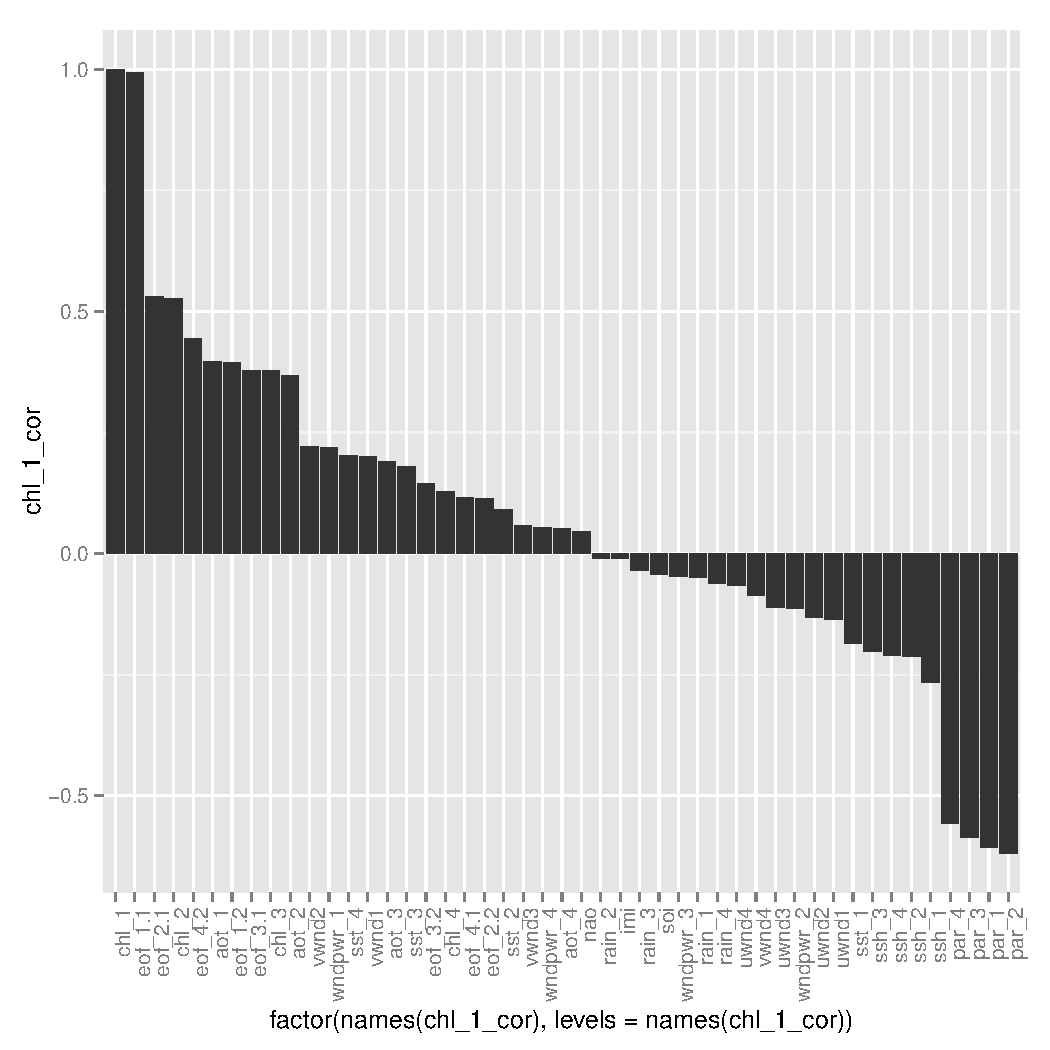
\includegraphics[width=\maxwidth]{figure/unnamed-chunk-2-1} 

\end{knitrout}

\subsection{Linear Regression}

\begin{knitrout}
\definecolor{shadecolor}{rgb}{0.969, 0.969, 0.969}\color{fgcolor}\begin{kframe}
\begin{alltt}
\hlkwd{summary}\hlstd{(}\hlkwd{lm}\hlstd{(chl_1}\hlopt{~}\hlstd{sst_1}\hlopt{+}\hlstd{par_1}\hlopt{+}\hlstd{par_2}\hlopt{+}\hlstd{par_3}\hlopt{+}\hlstd{par_4}\hlopt{+}\hlstd{ssh_1}\hlopt{+}\hlstd{ssh_2}\hlopt{+}\hlstd{ssh_3}\hlopt{+}\hlstd{ssh_4}\hlopt{+}\hlstd{aot_1}\hlopt{+}\hlstd{chl_2}\hlopt{+}\hlstd{chl_3}\hlopt{+}\hlstd{aot_2,} \hlkwc{data}\hlstd{=df))}
\end{alltt}
\begin{verbatim}
## 
## Call:
## lm(formula = chl_1 ~ sst_1 + par_1 + par_2 + par_3 + par_4 + 
##     ssh_1 + ssh_2 + ssh_3 + ssh_4 + aot_1 + chl_2 + chl_3 + aot_2, 
##     data = df)
## 
## Residuals:
##      Min       1Q   Median       3Q      Max 
## -0.46880 -0.15882 -0.02295  0.12204  1.14062 
## 
## Coefficients:
##              Estimate Std. Error t value Pr(>|t|)    
## (Intercept)  1.724701   0.402686   4.283 2.40e-05 ***
## sst_1       -0.036525   0.015986  -2.285 0.022941 *  
## par_1       -0.013776   0.007856  -1.754 0.080396 .  
## par_2       -0.016272   0.010875  -1.496 0.135490    
## par_3       -0.015442   0.013265  -1.164 0.245194    
## par_4        0.032885   0.009272   3.547 0.000445 ***
## ssh_1       -2.507153   0.632757  -3.962 9.04e-05 ***
## ssh_2        1.546300   0.691516   2.236 0.025990 *  
## ssh_3        0.934232   0.629504   1.484 0.138710    
## ssh_4       -1.346539   0.524133  -2.569 0.010620 *  
## aot_1        0.237522   0.554706   0.428 0.668779    
## chl_2        0.460944   0.091576   5.033 7.80e-07 ***
## chl_3       -0.131964   0.088685  -1.488 0.137673    
## aot_2        1.088669   0.520563   2.091 0.037236 *  
## ---
## Signif. codes:  0 '***' 0.001 '**' 0.01 '*' 0.05 '.' 0.1 ' ' 1
## 
## Residual standard error: 0.2364 on 342 degrees of freedom
##   (108 observations deleted due to missingness)
## Multiple R-squared:  0.5333,	Adjusted R-squared:  0.5156 
## F-statistic: 30.07 on 13 and 342 DF,  p-value: < 2.2e-16
\end{verbatim}
\end{kframe}
\end{knitrout}

\subsection{Chlorophyll and chlorophyll}

\begin{knitrout}
\definecolor{shadecolor}{rgb}{0.969, 0.969, 0.969}\color{fgcolor}\begin{kframe}
\begin{alltt}
\hlkwd{qplot}\hlstd{(chl_1, chl_2,} \hlkwc{data}\hlstd{=df,} \hlkwc{geom}\hlstd{=}\hlkwd{c}\hlstd{(}\hlstr{'point'}\hlstd{,} \hlstr{'smooth'}\hlstd{),} \hlkwc{method}\hlstd{=}\hlstr{'lm'}\hlstd{,} \hlkwc{formula}\hlstd{=y}\hlopt{~}\hlstd{x)}
\end{alltt}
\end{kframe}
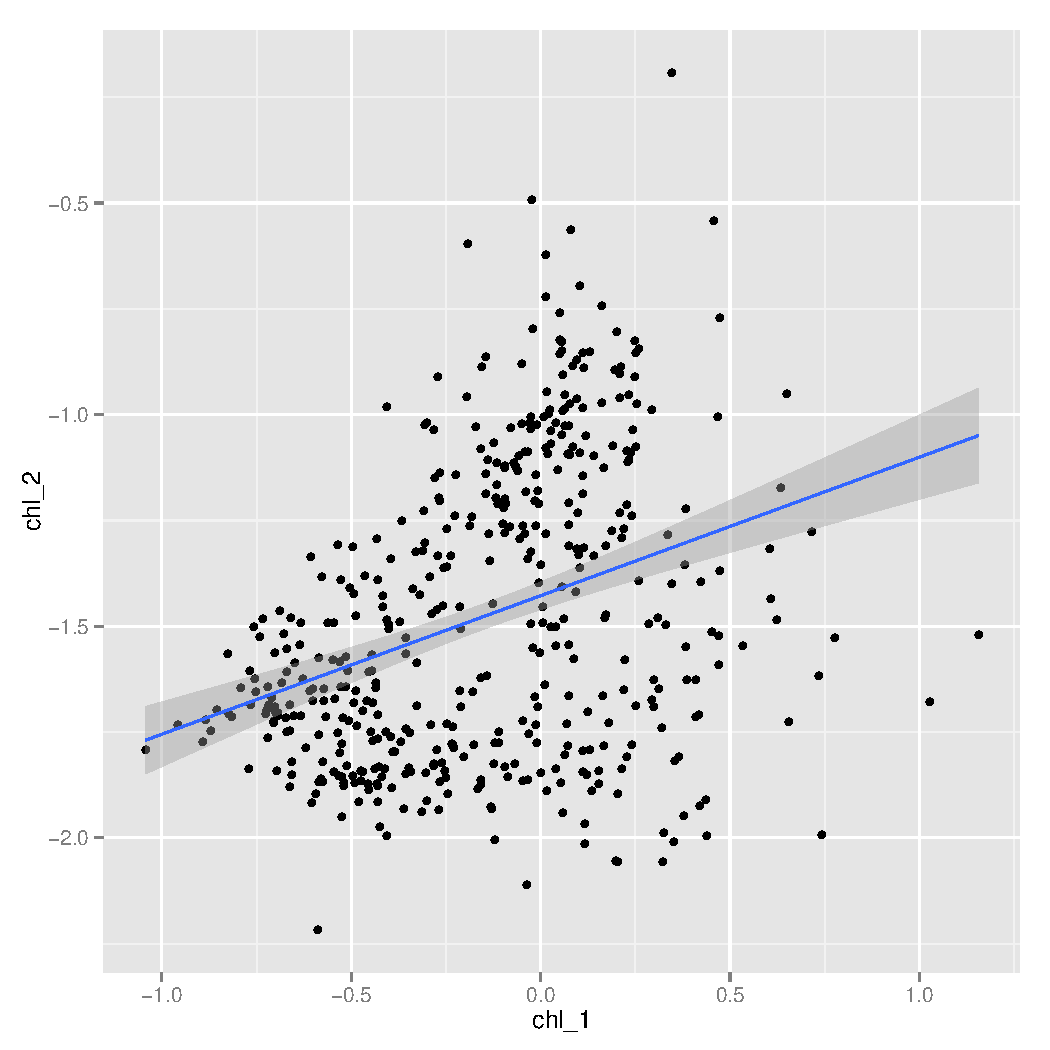
\includegraphics[width=\maxwidth]{figure/unnamed-chunk-4-1} 
\begin{kframe}\begin{alltt}
\hlcom{## Correlation coefficient}
\hlkwd{cor}\hlstd{(df}\hlopt{$}\hlstd{chl_1, df}\hlopt{$}\hlstd{chl_2,} \hlkwc{use}\hlstd{=}\hlstr{'complete.obs'}\hlstd{)}
\end{alltt}
\begin{verbatim}
## [1] 0.3404985
\end{verbatim}
\begin{alltt}
\hlkwd{ccf}\hlstd{(df}\hlopt{$}\hlstd{chl_1, df}\hlopt{$}\hlstd{chl_2)}
\end{alltt}
\end{kframe}
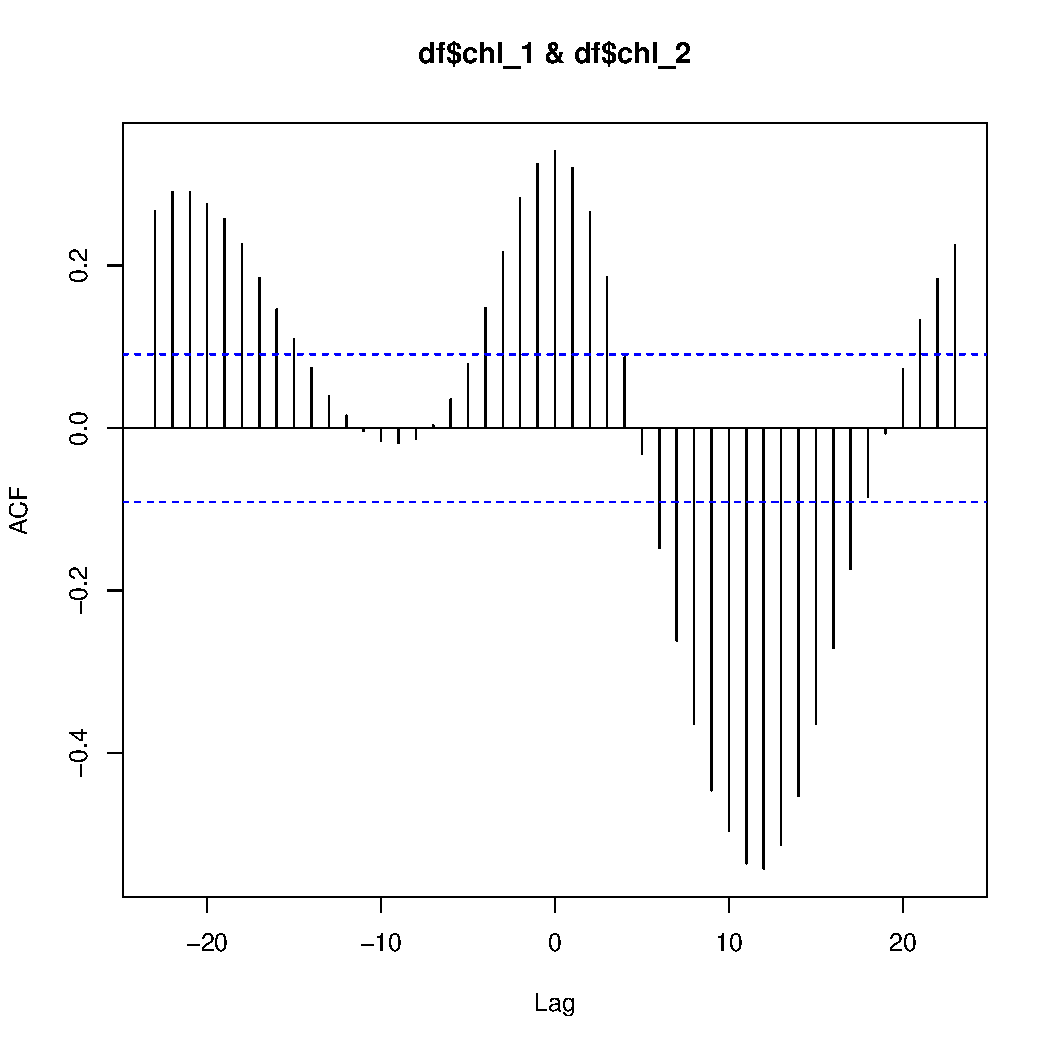
\includegraphics[width=\maxwidth]{figure/unnamed-chunk-4-2} 

\end{knitrout}

\begin{knitrout}
\definecolor{shadecolor}{rgb}{0.969, 0.969, 0.969}\color{fgcolor}\begin{kframe}
\begin{alltt}
\hlkwd{qplot}\hlstd{(chl_1, chl_3,} \hlkwc{data}\hlstd{=df,} \hlkwc{geom}\hlstd{=}\hlkwd{c}\hlstd{(}\hlstr{'point'}\hlstd{,} \hlstr{'smooth'}\hlstd{),} \hlkwc{method}\hlstd{=}\hlstr{'lm'}\hlstd{,} \hlkwc{formula}\hlstd{=y}\hlopt{~}\hlstd{x)}
\end{alltt}
\end{kframe}
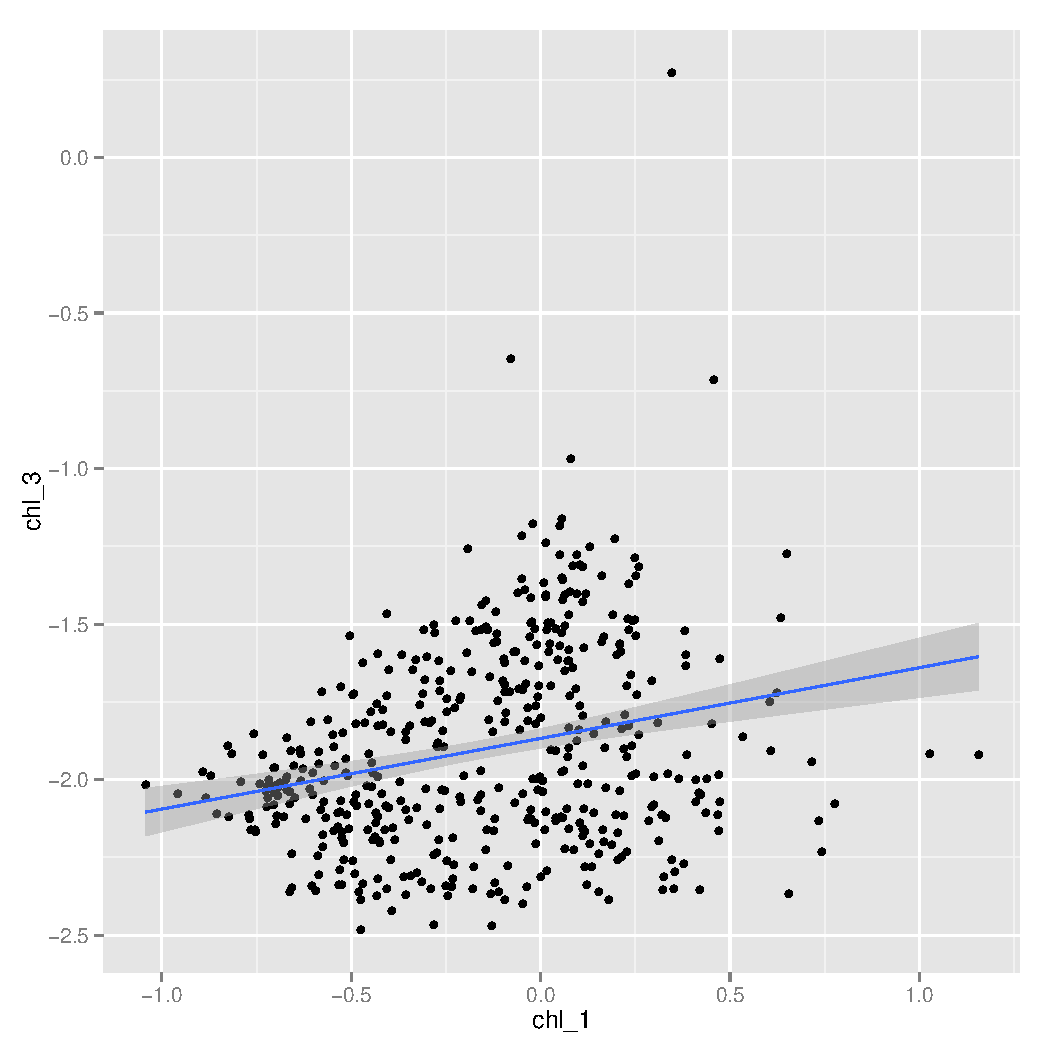
\includegraphics[width=\maxwidth]{figure/unnamed-chunk-5-1} 
\begin{kframe}\begin{alltt}
\hlcom{## Correlation coefficient}
\hlkwd{cor}\hlstd{(df}\hlopt{$}\hlstd{chl_1, df}\hlopt{$}\hlstd{chl_3,} \hlkwc{use}\hlstd{=}\hlstr{'complete.obs'}\hlstd{)}
\end{alltt}
\begin{verbatim}
## [1] 0.2533124
\end{verbatim}
\begin{alltt}
\hlkwd{ccf}\hlstd{(df}\hlopt{$}\hlstd{chl_1, df}\hlopt{$}\hlstd{chl_3)}
\end{alltt}
\end{kframe}
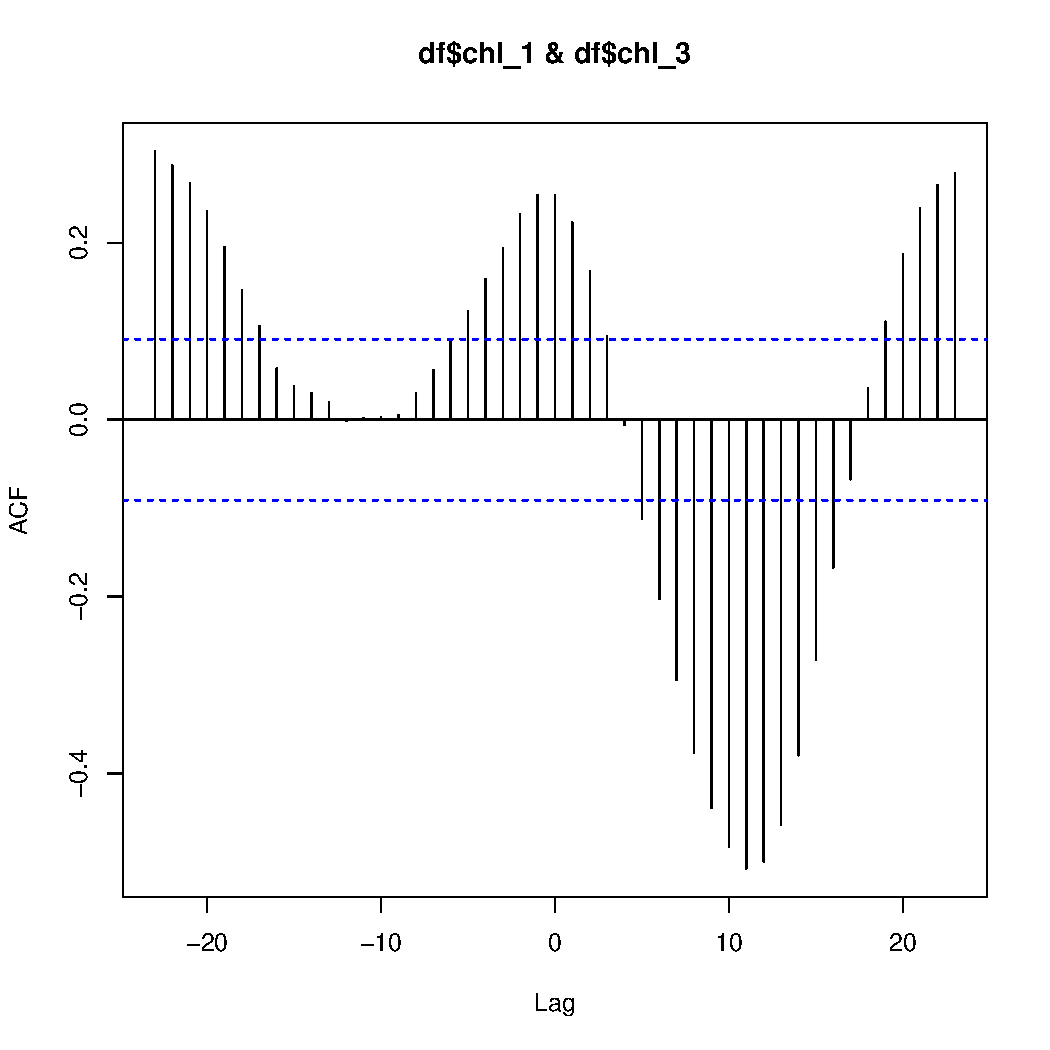
\includegraphics[width=\maxwidth]{figure/unnamed-chunk-5-2} 

\end{knitrout}

\begin{knitrout}
\definecolor{shadecolor}{rgb}{0.969, 0.969, 0.969}\color{fgcolor}\begin{kframe}
\begin{alltt}
\hlkwd{qplot}\hlstd{(chl_1, chl_4,} \hlkwc{data}\hlstd{=df,} \hlkwc{geom}\hlstd{=}\hlkwd{c}\hlstd{(}\hlstr{'point'}\hlstd{,} \hlstr{'smooth'}\hlstd{),} \hlkwc{method}\hlstd{=}\hlstr{'lm'}\hlstd{,} \hlkwc{formula}\hlstd{=y}\hlopt{~}\hlstd{x)}
\end{alltt}
\end{kframe}
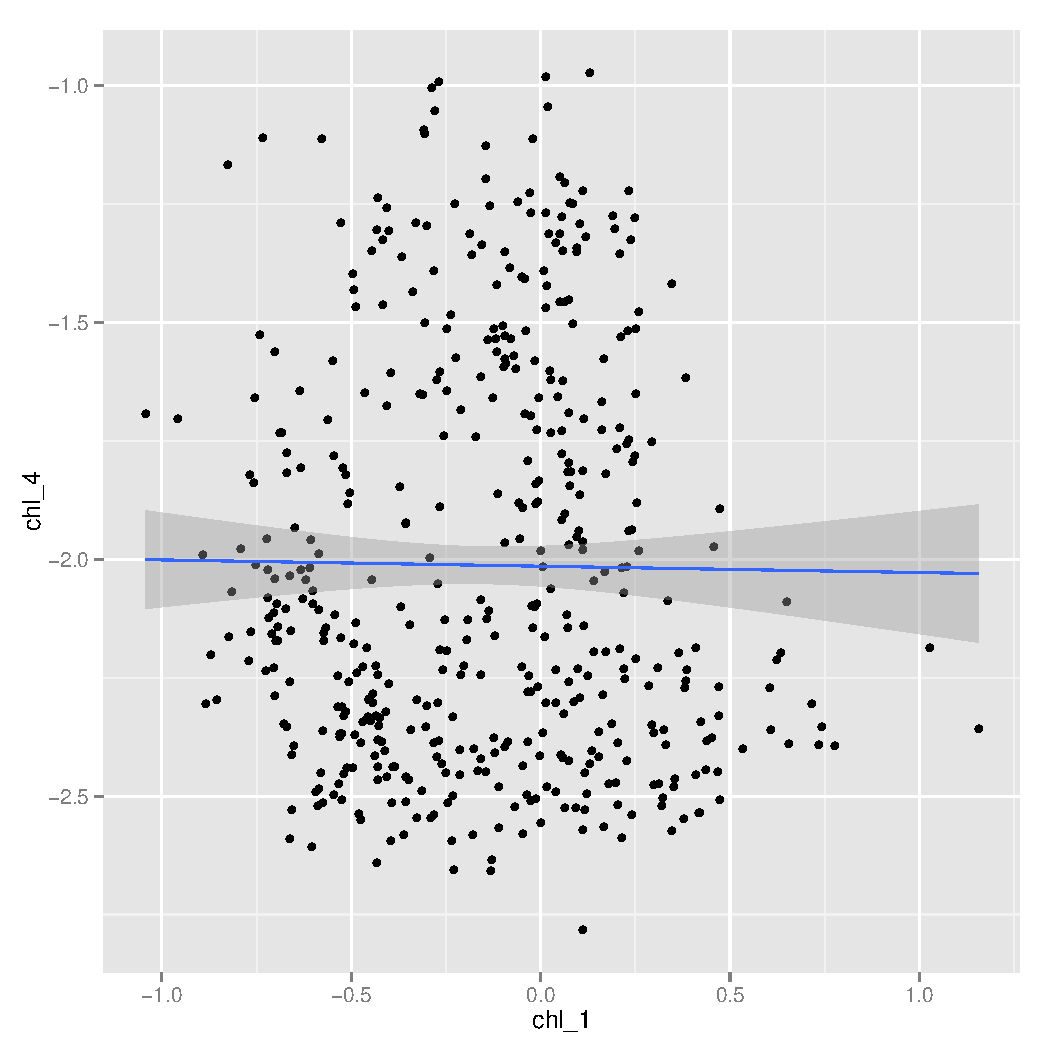
\includegraphics[width=\maxwidth]{figure/unnamed-chunk-6-1} 
\begin{kframe}\begin{alltt}
\hlcom{## Correlation coefficient}
\hlkwd{cor}\hlstd{(df}\hlopt{$}\hlstd{chl_1, df}\hlopt{$}\hlstd{chl_4,} \hlkwc{use}\hlstd{=}\hlstr{'complete.obs'}\hlstd{)}
\end{alltt}
\begin{verbatim}
## [1] -0.01136072
\end{verbatim}
\begin{alltt}
\hlkwd{ccf}\hlstd{(df}\hlopt{$}\hlstd{chl_1, df}\hlopt{$}\hlstd{chl_4)}
\end{alltt}
\end{kframe}
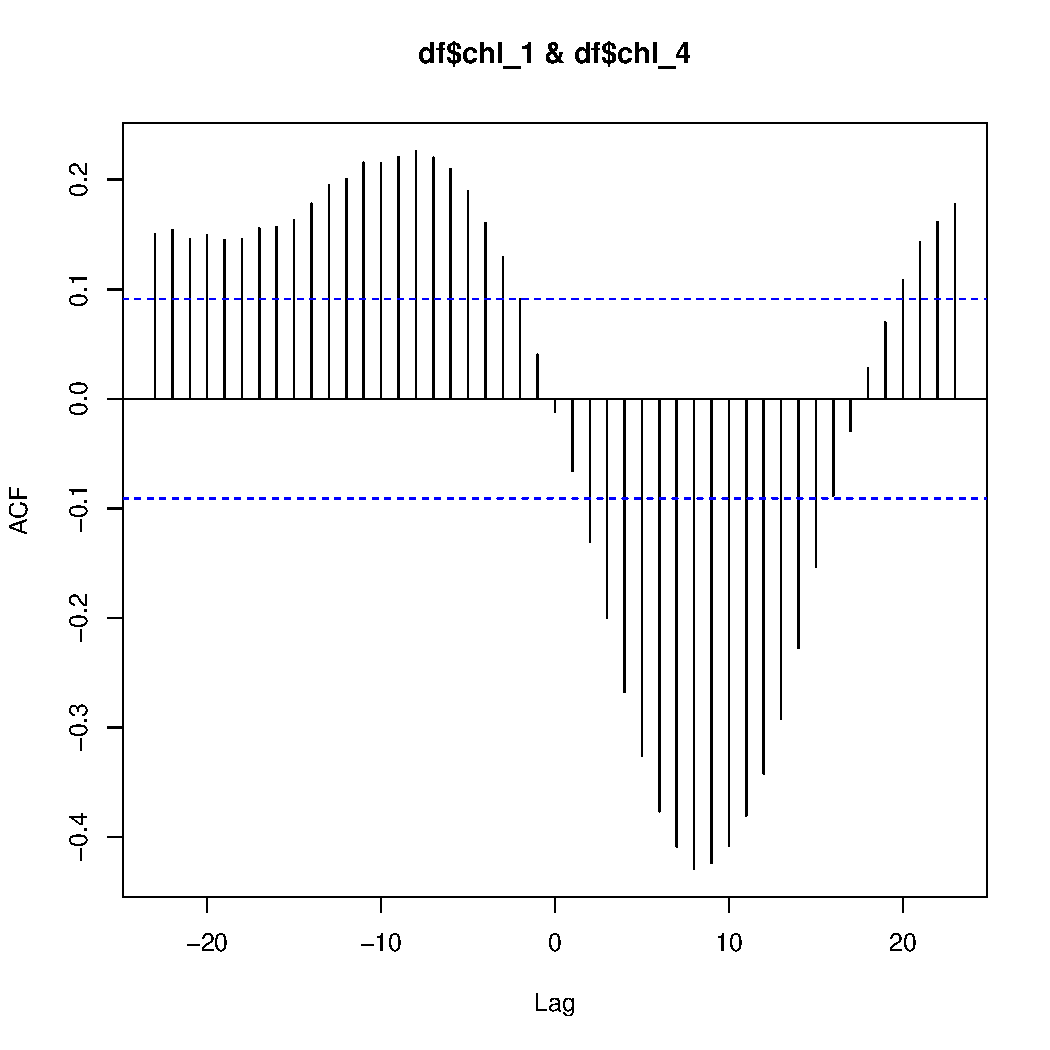
\includegraphics[width=\maxwidth]{figure/unnamed-chunk-6-2} 

\end{knitrout}

\subsection{Chlorophyll and temperatures}

\begin{knitrout}
\definecolor{shadecolor}{rgb}{0.969, 0.969, 0.969}\color{fgcolor}\begin{kframe}
\begin{alltt}
\hlkwd{qplot}\hlstd{(chl_1, sst_1,} \hlkwc{data}\hlstd{=df,} \hlkwc{geom}\hlstd{=}\hlkwd{c}\hlstd{(}\hlstr{'point'}\hlstd{,} \hlstr{'smooth'}\hlstd{),} \hlkwc{method}\hlstd{=}\hlstr{'lm'}\hlstd{,} \hlkwc{formula}\hlstd{=y}\hlopt{~}\hlstd{x)}
\end{alltt}


{\ttfamily\noindent\color{warningcolor}{\#\# Warning: Removed 1 rows containing missing values (stat\_smooth).}}

{\ttfamily\noindent\color{warningcolor}{\#\# Warning: Removed 1 rows containing missing values (geom\_point).}}\end{kframe}
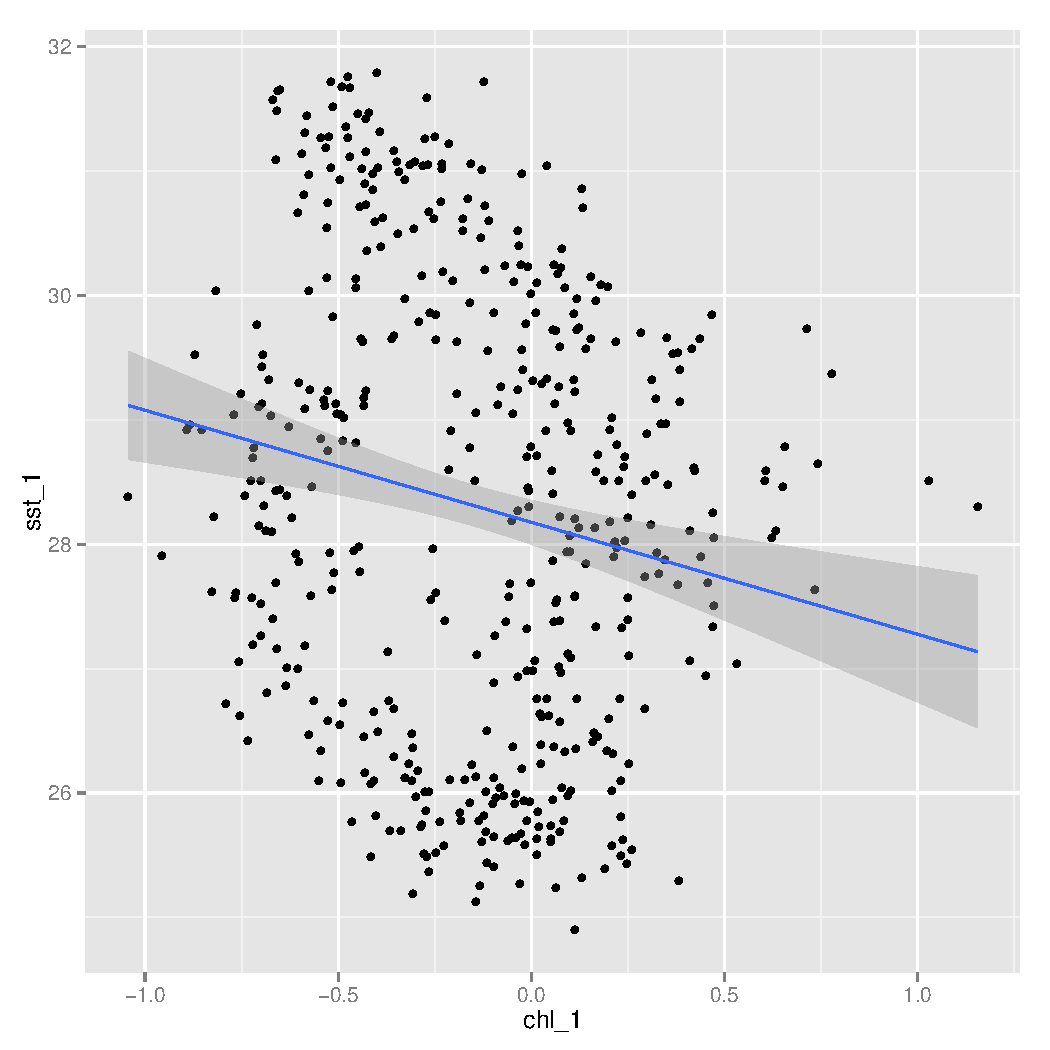
\includegraphics[width=\maxwidth]{figure/unnamed-chunk-7-1} 
\begin{kframe}\begin{alltt}
\hlcom{## Correlation coefficient}
\hlkwd{cor}\hlstd{(df}\hlopt{$}\hlstd{chl_1, df}\hlopt{$}\hlstd{sst_1,} \hlkwc{use}\hlstd{=}\hlstr{'complete.obs'}\hlstd{)}
\end{alltt}
\begin{verbatim}
## [1] -0.1792175
\end{verbatim}
\begin{alltt}
\hlkwd{ccf}\hlstd{(df}\hlopt{$}\hlstd{chl_1, df}\hlopt{$}\hlstd{sst_1,} \hlkwc{na.action}\hlstd{=na.pass)}
\end{alltt}
\end{kframe}
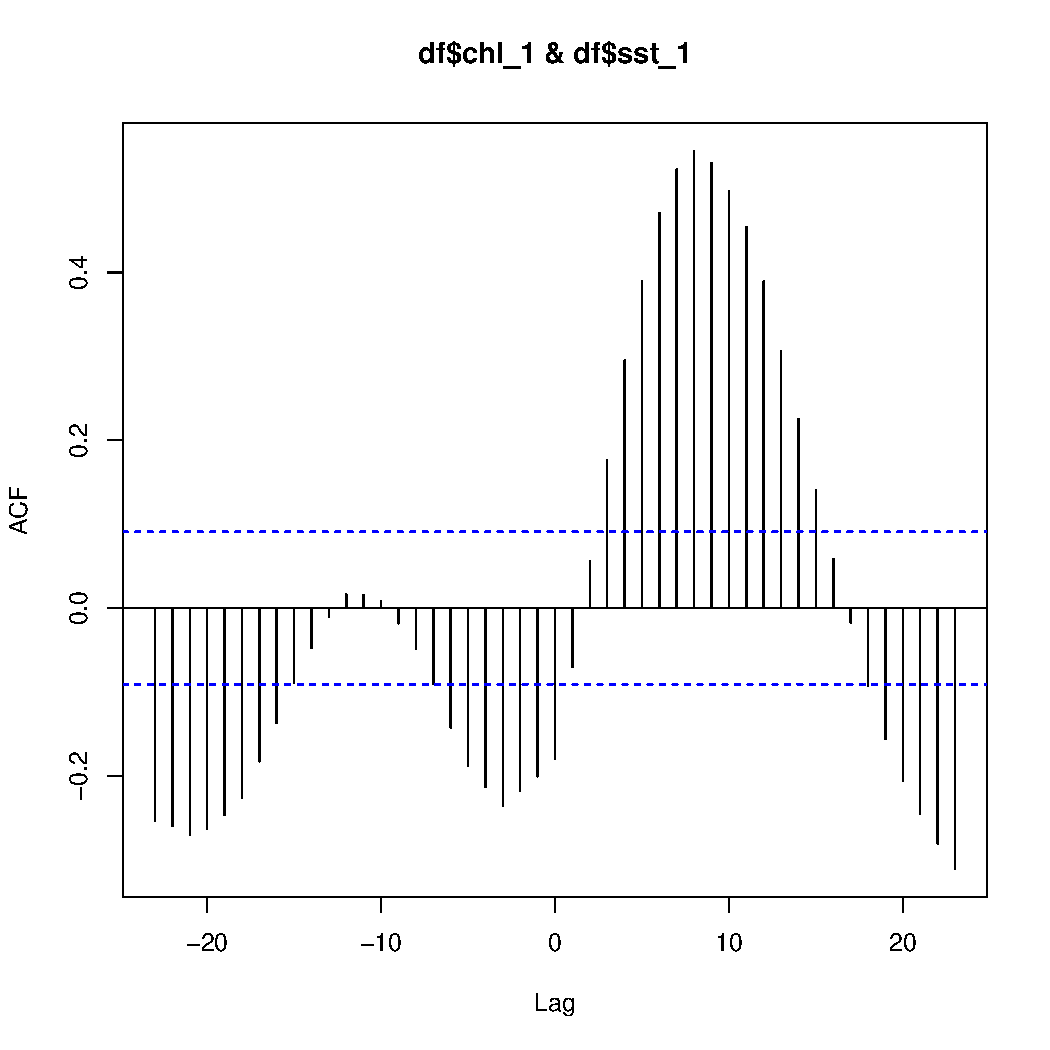
\includegraphics[width=\maxwidth]{figure/unnamed-chunk-7-2} 

\end{knitrout}

\begin{knitrout}
\definecolor{shadecolor}{rgb}{0.969, 0.969, 0.969}\color{fgcolor}\begin{kframe}
\begin{alltt}
\hlkwd{qplot}\hlstd{(chl_1, sst_2,} \hlkwc{data}\hlstd{=df,} \hlkwc{geom}\hlstd{=}\hlkwd{c}\hlstd{(}\hlstr{'point'}\hlstd{,} \hlstr{'smooth'}\hlstd{),} \hlkwc{method}\hlstd{=}\hlstr{'lm'}\hlstd{,} \hlkwc{formula}\hlstd{=y}\hlopt{~}\hlstd{x)}
\end{alltt}


{\ttfamily\noindent\color{warningcolor}{\#\# Warning: Removed 1 rows containing missing values (stat\_smooth).}}

{\ttfamily\noindent\color{warningcolor}{\#\# Warning: Removed 1 rows containing missing values (geom\_point).}}\end{kframe}
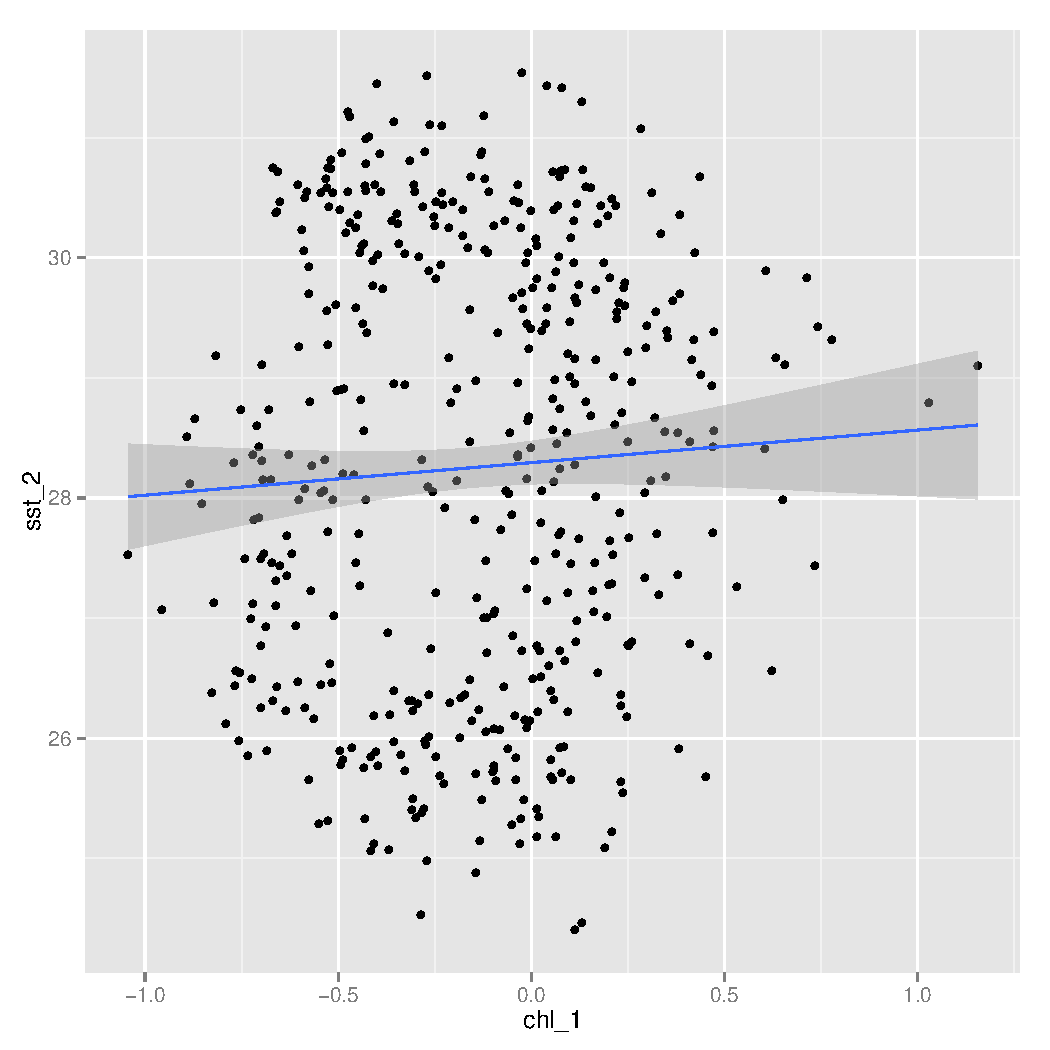
\includegraphics[width=\maxwidth]{figure/unnamed-chunk-8-1} 
\begin{kframe}\begin{alltt}
\hlcom{## Correlation coefficient}
\hlkwd{cor}\hlstd{(df}\hlopt{$}\hlstd{chl_1, df}\hlopt{$}\hlstd{sst_2,} \hlkwc{use}\hlstd{=}\hlstr{'complete.obs'}\hlstd{)}
\end{alltt}
\begin{verbatim}
## [1] 0.05444485
\end{verbatim}
\begin{alltt}
\hlkwd{ccf}\hlstd{(df}\hlopt{$}\hlstd{chl_1, df}\hlopt{$}\hlstd{sst_2,} \hlkwc{na.action}\hlstd{=na.pass)}
\end{alltt}
\end{kframe}
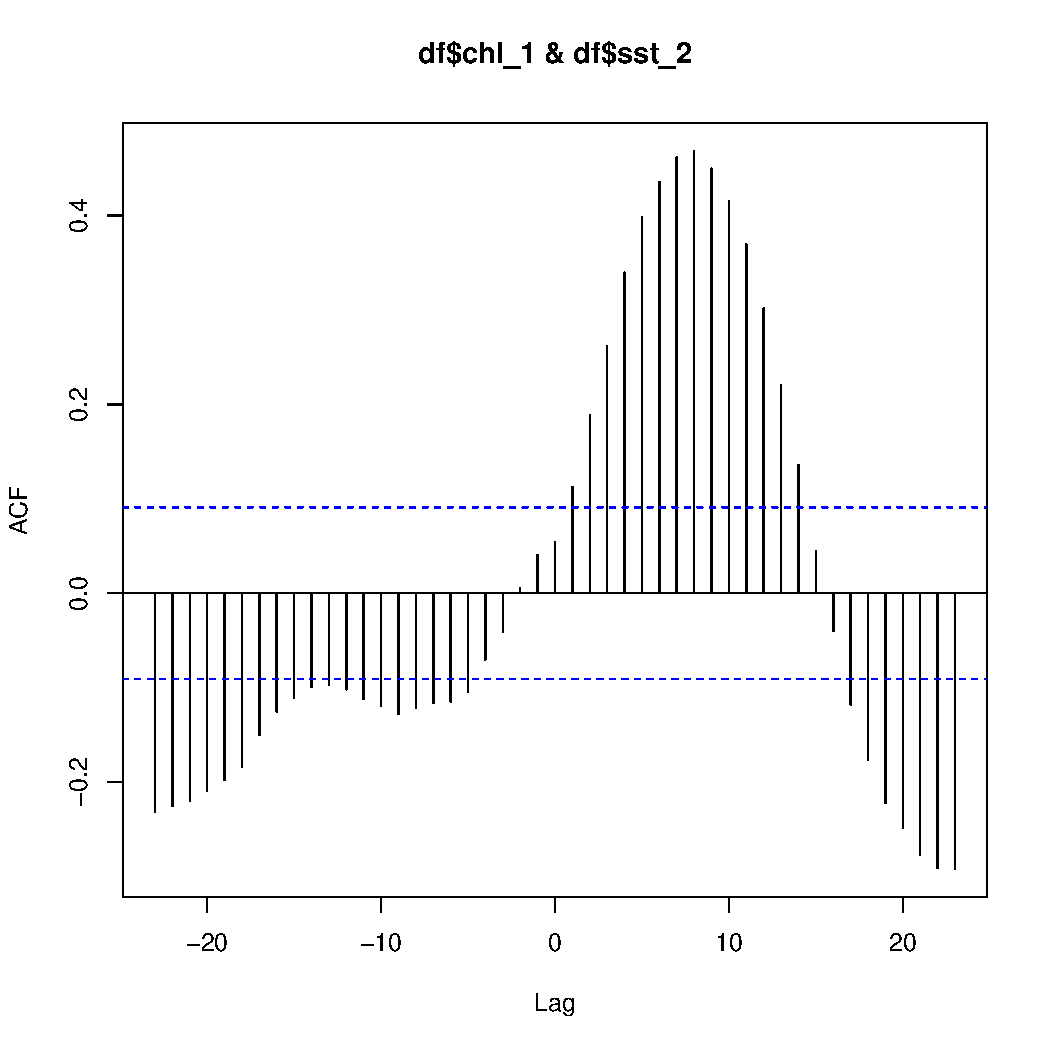
\includegraphics[width=\maxwidth]{figure/unnamed-chunk-8-2} 

\end{knitrout}

\begin{knitrout}
\definecolor{shadecolor}{rgb}{0.969, 0.969, 0.969}\color{fgcolor}\begin{kframe}
\begin{alltt}
\hlkwd{qplot}\hlstd{(chl_1, sst_3,} \hlkwc{data}\hlstd{=df,} \hlkwc{geom}\hlstd{=}\hlkwd{c}\hlstd{(}\hlstr{'point'}\hlstd{,} \hlstr{'smooth'}\hlstd{),} \hlkwc{method}\hlstd{=}\hlstr{'lm'}\hlstd{,} \hlkwc{formula}\hlstd{=y}\hlopt{~}\hlstd{x)}
\end{alltt}


{\ttfamily\noindent\color{warningcolor}{\#\# Warning: Removed 1 rows containing missing values (stat\_smooth).}}

{\ttfamily\noindent\color{warningcolor}{\#\# Warning: Removed 1 rows containing missing values (geom\_point).}}\end{kframe}
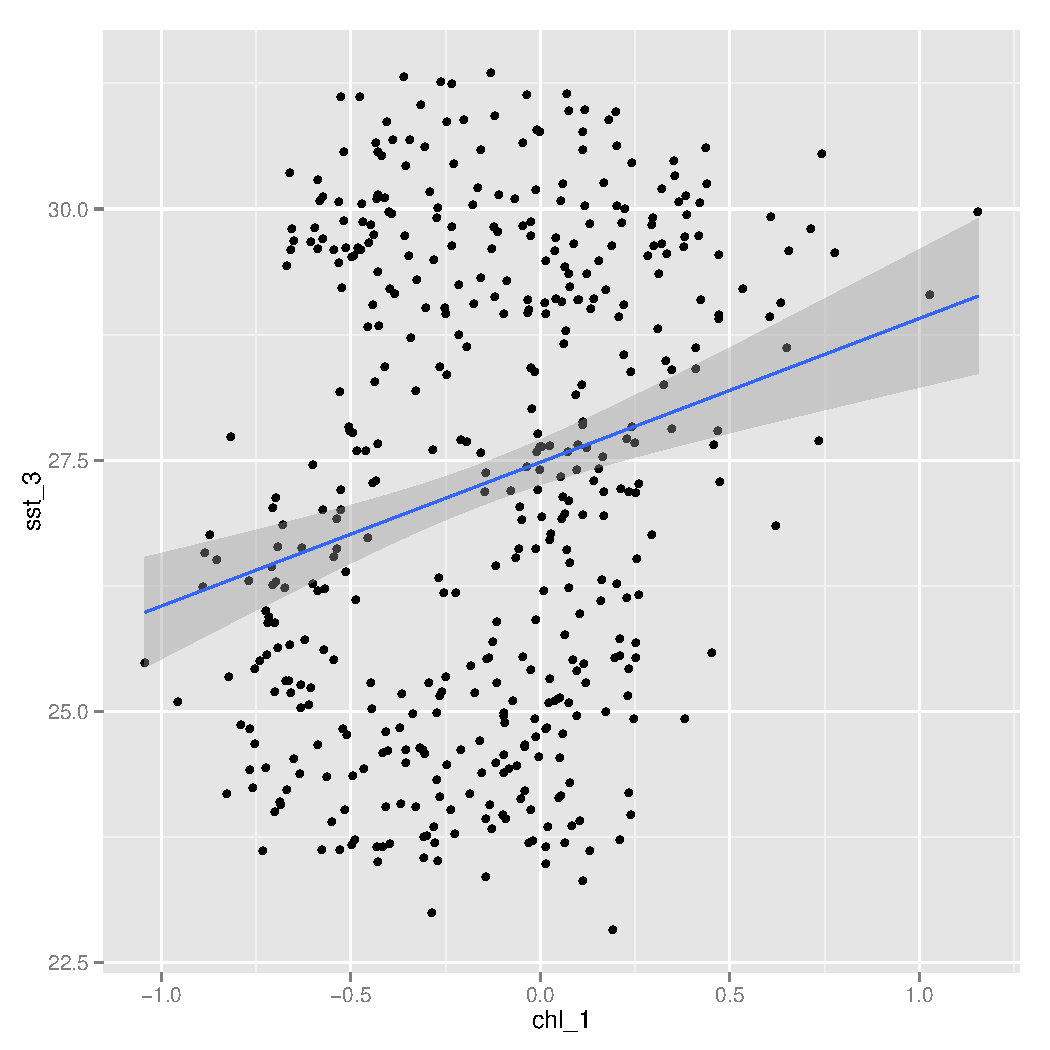
\includegraphics[width=\maxwidth]{figure/unnamed-chunk-9-1} 
\begin{kframe}\begin{alltt}
\hlcom{## Correlation coefficient}
\hlkwd{cor}\hlstd{(df}\hlopt{$}\hlstd{chl_1, df}\hlopt{$}\hlstd{sst_3,} \hlkwc{use}\hlstd{=}\hlstr{'complete.obs'}\hlstd{)}
\end{alltt}
\begin{verbatim}
## [1] 0.2245816
\end{verbatim}
\begin{alltt}
\hlkwd{ccf}\hlstd{(df}\hlopt{$}\hlstd{chl_1, df}\hlopt{$}\hlstd{sst_3,} \hlkwc{na.action}\hlstd{=na.pass)}
\end{alltt}
\end{kframe}
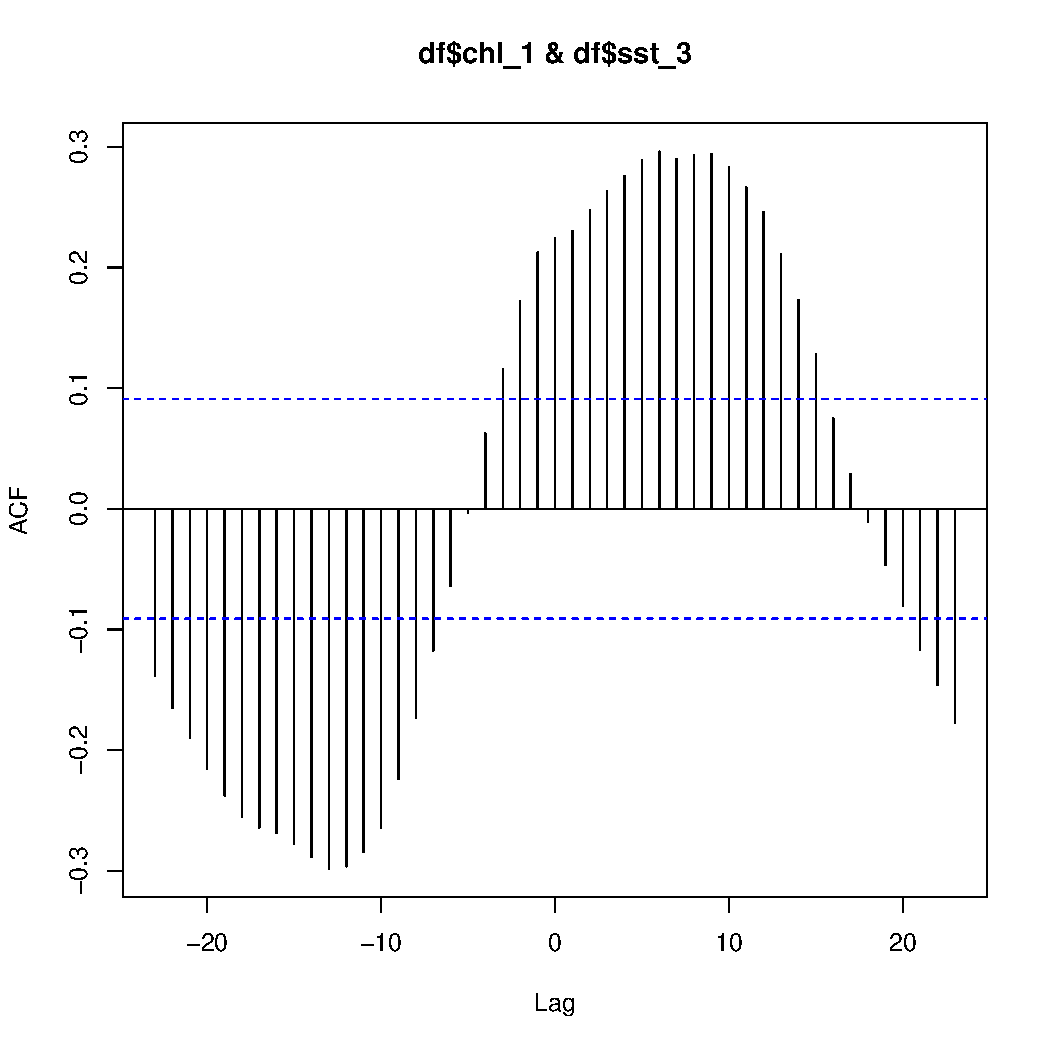
\includegraphics[width=\maxwidth]{figure/unnamed-chunk-9-2} 

\end{knitrout}

\begin{knitrout}
\definecolor{shadecolor}{rgb}{0.969, 0.969, 0.969}\color{fgcolor}\begin{kframe}
\begin{alltt}
\hlkwd{qplot}\hlstd{(chl_1, sst_4,} \hlkwc{data}\hlstd{=df,} \hlkwc{geom}\hlstd{=}\hlkwd{c}\hlstd{(}\hlstr{'point'}\hlstd{,} \hlstr{'smooth'}\hlstd{),} \hlkwc{method}\hlstd{=}\hlstr{'lm'}\hlstd{,} \hlkwc{formula}\hlstd{=y}\hlopt{~}\hlstd{x)}
\end{alltt}


{\ttfamily\noindent\color{warningcolor}{\#\# Warning: Removed 1 rows containing missing values (stat\_smooth).}}

{\ttfamily\noindent\color{warningcolor}{\#\# Warning: Removed 1 rows containing missing values (geom\_point).}}\end{kframe}
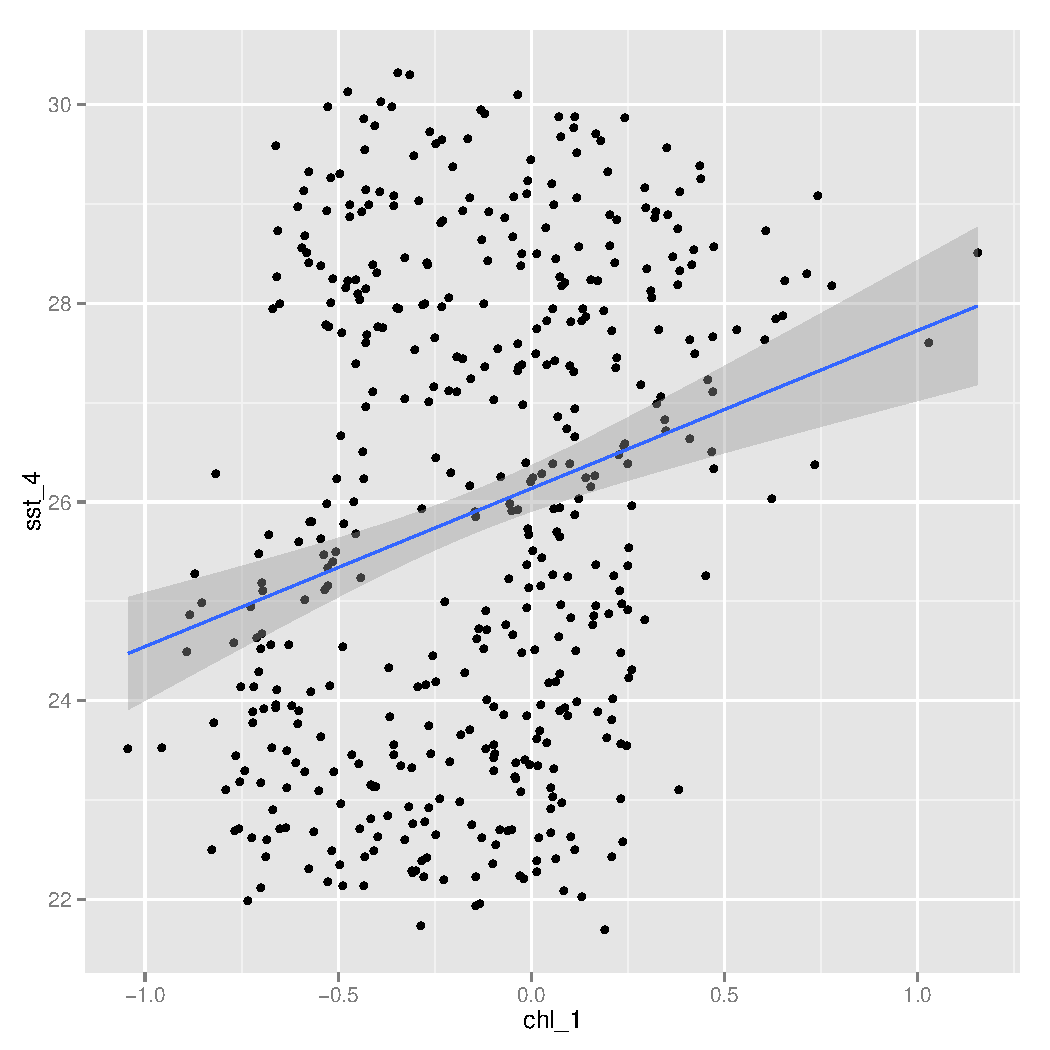
\includegraphics[width=\maxwidth]{figure/unnamed-chunk-10-1} 
\begin{kframe}\begin{alltt}
\hlcom{## Correlation coefficient}
\hlkwd{cor}\hlstd{(df}\hlopt{$}\hlstd{chl_1, df}\hlopt{$}\hlstd{sst_4,} \hlkwc{use}\hlstd{=}\hlstr{'complete.obs'}\hlstd{)}
\end{alltt}
\begin{verbatim}
## [1] 0.2414238
\end{verbatim}
\begin{alltt}
\hlkwd{ccf}\hlstd{(df}\hlopt{$}\hlstd{chl_1, df}\hlopt{$}\hlstd{sst_4,} \hlkwc{na.action}\hlstd{=na.pass)}
\end{alltt}
\end{kframe}
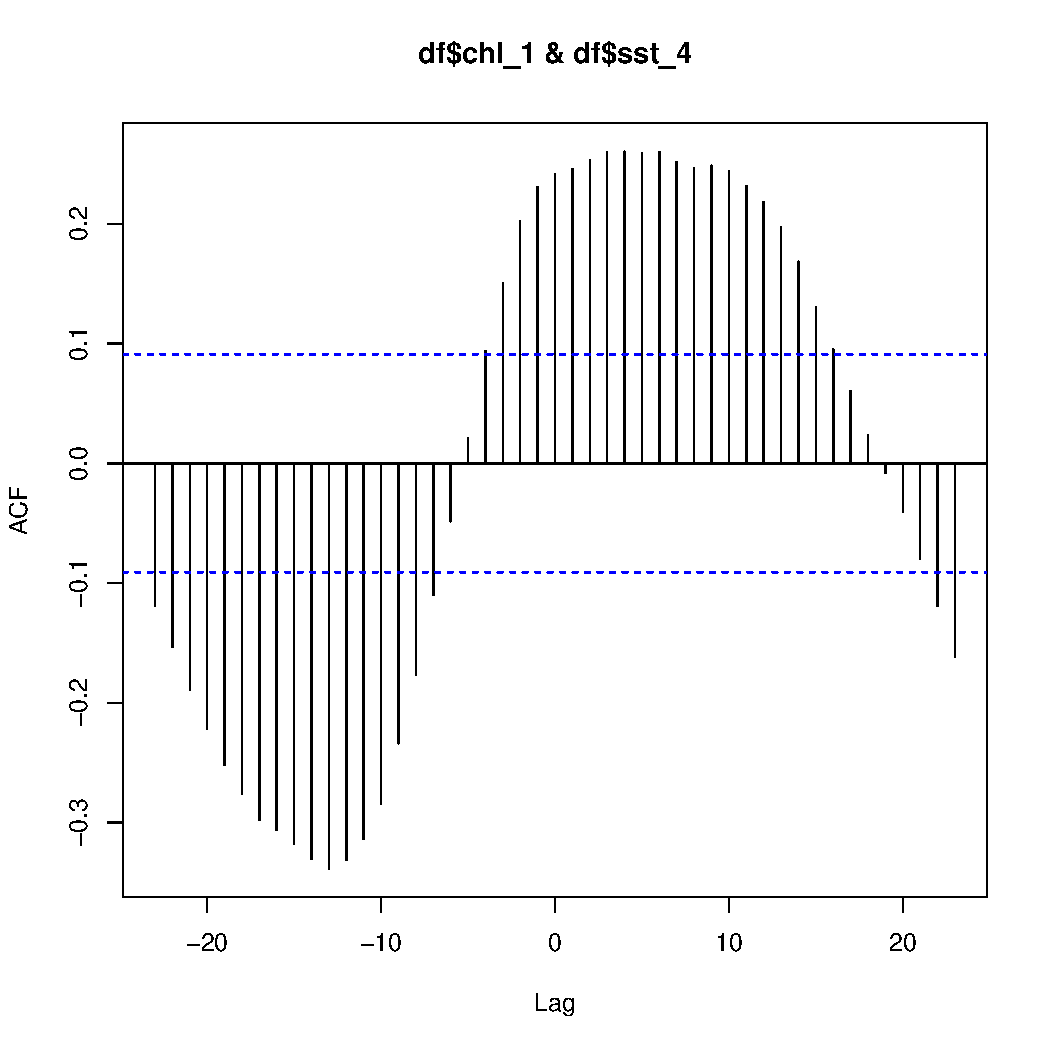
\includegraphics[width=\maxwidth]{figure/unnamed-chunk-10-2} 

\end{knitrout}

\subsection{Chlorophyll and SLA}

\begin{knitrout}
\definecolor{shadecolor}{rgb}{0.969, 0.969, 0.969}\color{fgcolor}\begin{kframe}
\begin{alltt}
\hlkwd{qplot}\hlstd{(chl_1, ssh_1,} \hlkwc{data}\hlstd{=df,} \hlkwc{geom}\hlstd{=}\hlkwd{c}\hlstd{(}\hlstr{'point'}\hlstd{,} \hlstr{'smooth'}\hlstd{),} \hlkwc{method}\hlstd{=}\hlstr{'lm'}\hlstd{,} \hlkwc{formula}\hlstd{=y}\hlopt{~}\hlstd{x)}
\end{alltt}
\end{kframe}
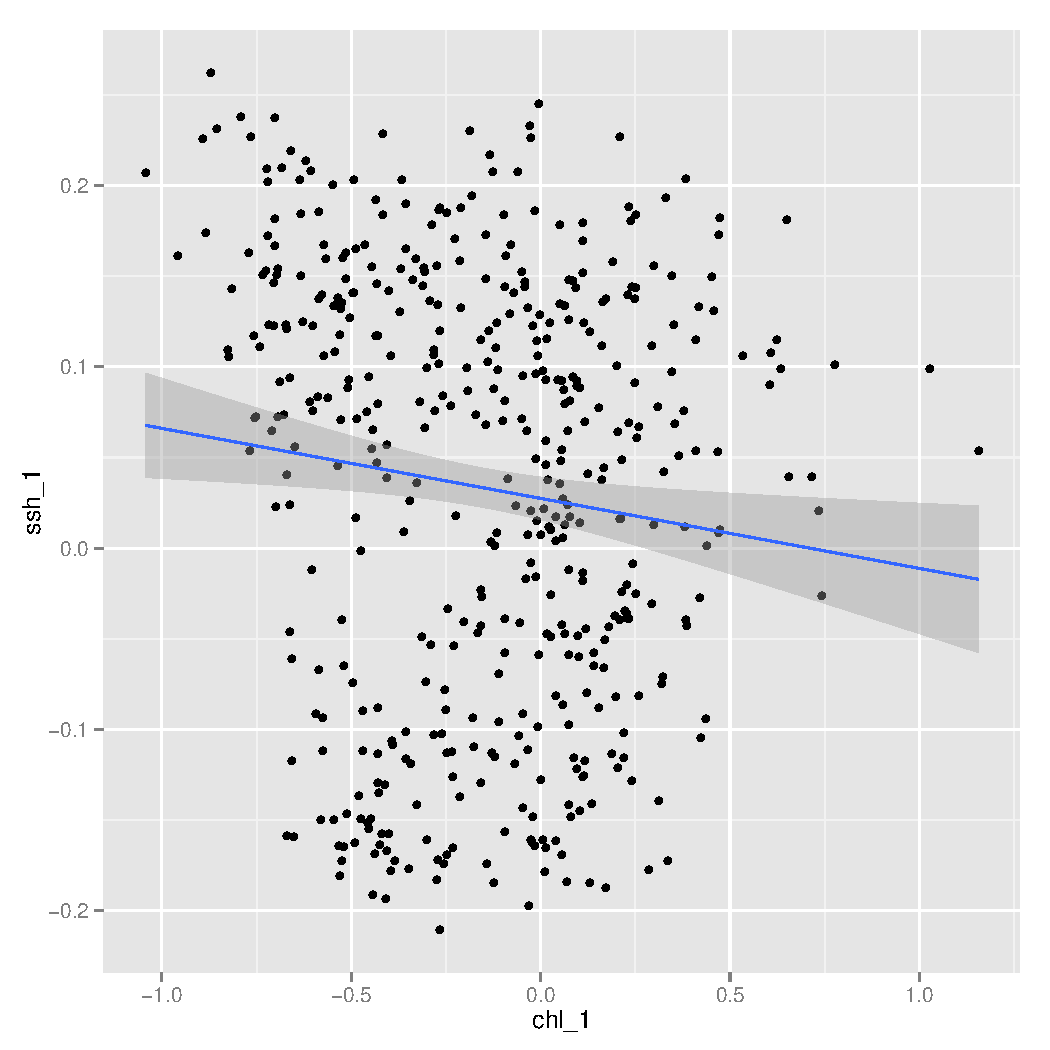
\includegraphics[width=\maxwidth]{figure/unnamed-chunk-11-1} 
\begin{kframe}\begin{alltt}
\hlcom{## Correlation coefficient}
\hlkwd{cor}\hlstd{(df}\hlopt{$}\hlstd{chl_1, df}\hlopt{$}\hlstd{ssh_1,} \hlkwc{use}\hlstd{=}\hlstr{'complete.obs'}\hlstd{)}
\end{alltt}
\begin{verbatim}
## [1] -0.1173844
\end{verbatim}
\begin{alltt}
\hlkwd{ccf}\hlstd{(df}\hlopt{$}\hlstd{chl_1, df}\hlopt{$}\hlstd{ssh_1,} \hlkwc{na.action}\hlstd{=na.pass)}
\end{alltt}
\end{kframe}
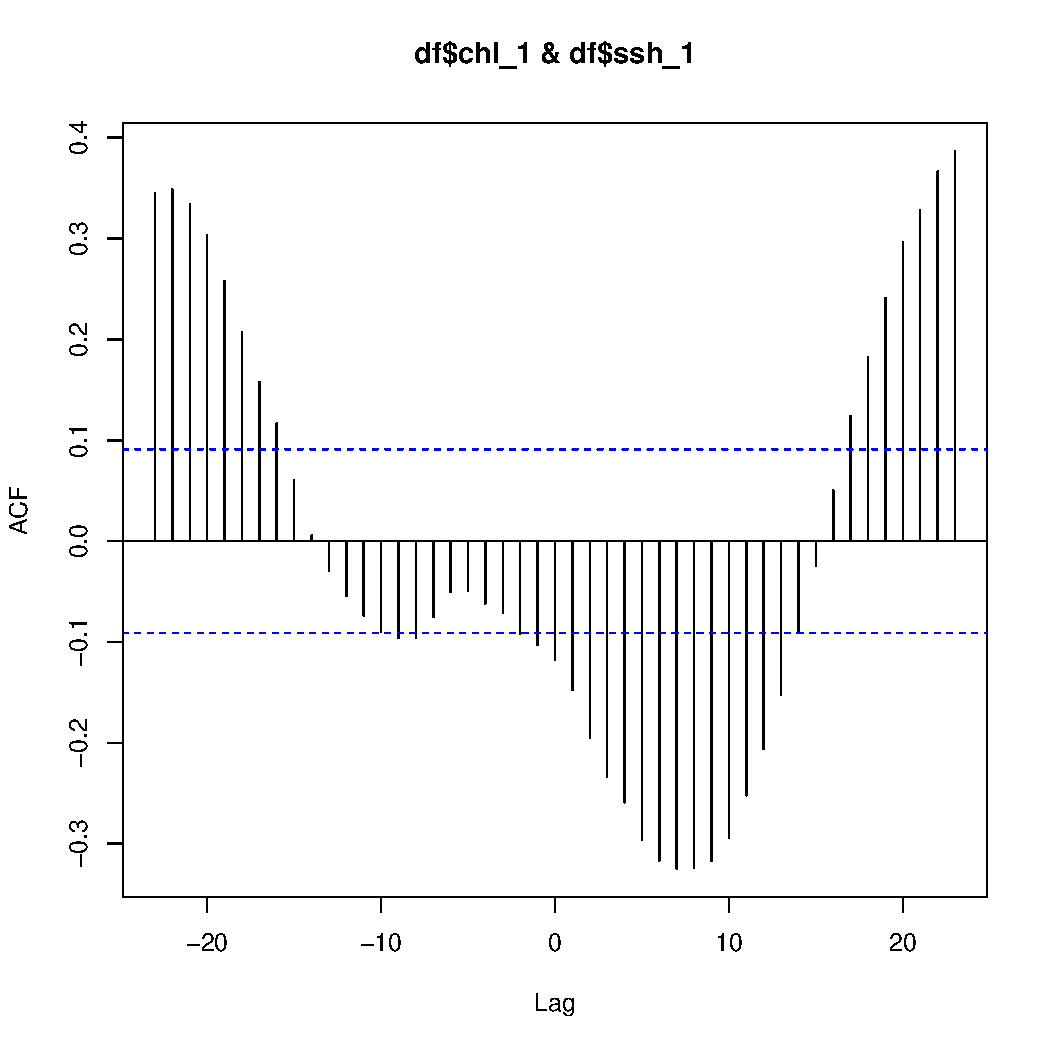
\includegraphics[width=\maxwidth]{figure/unnamed-chunk-11-2} 

\end{knitrout}

\begin{knitrout}
\definecolor{shadecolor}{rgb}{0.969, 0.969, 0.969}\color{fgcolor}\begin{kframe}
\begin{alltt}
\hlkwd{qplot}\hlstd{(chl_1, ssh_2,} \hlkwc{data}\hlstd{=df,} \hlkwc{geom}\hlstd{=}\hlkwd{c}\hlstd{(}\hlstr{'point'}\hlstd{,} \hlstr{'smooth'}\hlstd{),} \hlkwc{method}\hlstd{=}\hlstr{'lm'}\hlstd{,} \hlkwc{formula}\hlstd{=y}\hlopt{~}\hlstd{x)}
\end{alltt}
\end{kframe}
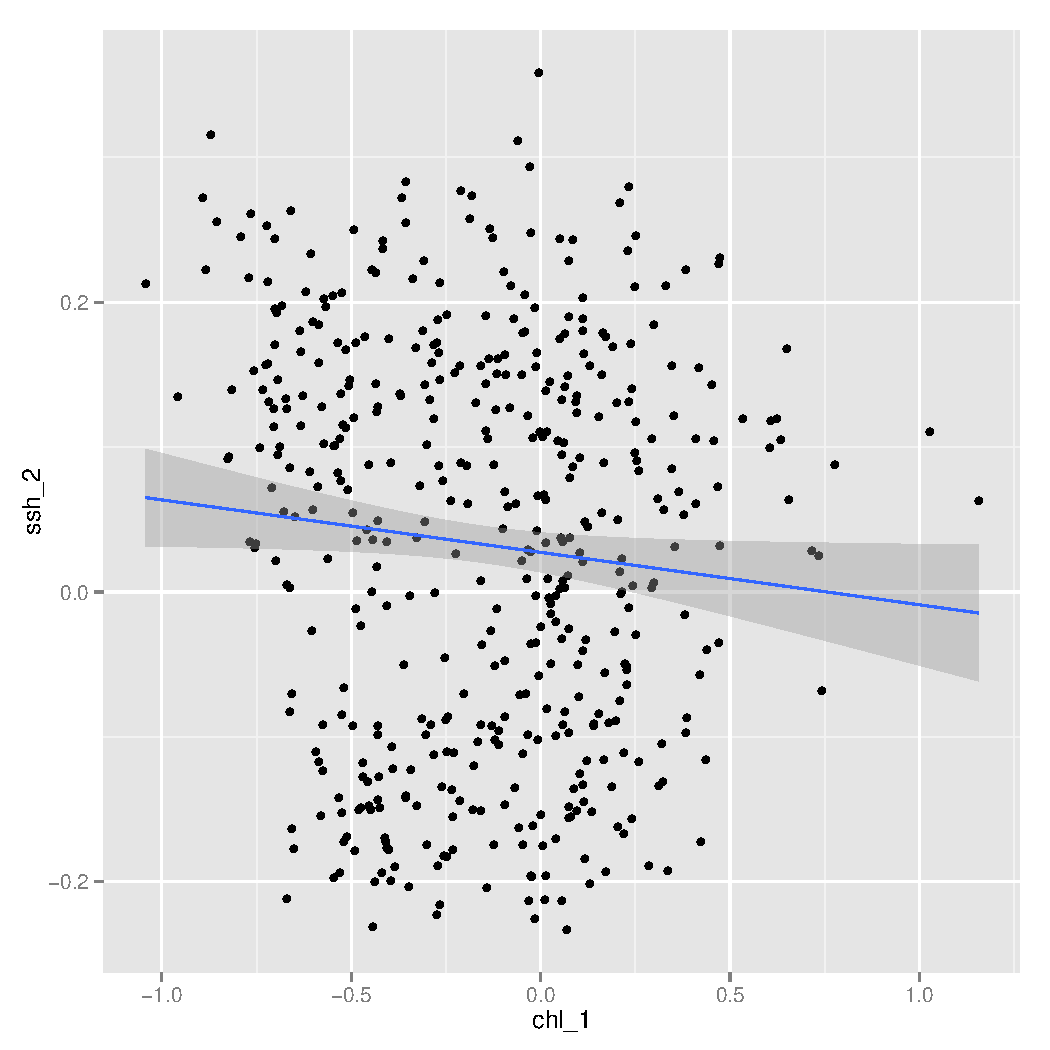
\includegraphics[width=\maxwidth]{figure/unnamed-chunk-12-1} 
\begin{kframe}\begin{alltt}
\hlcom{## Correlation coefficient}
\hlkwd{cor}\hlstd{(df}\hlopt{$}\hlstd{chl_1, df}\hlopt{$}\hlstd{ssh_2,} \hlkwc{use}\hlstd{=}\hlstr{'complete.obs'}\hlstd{)}
\end{alltt}
\begin{verbatim}
## [1] -0.09501634
\end{verbatim}
\begin{alltt}
\hlkwd{ccf}\hlstd{(df}\hlopt{$}\hlstd{chl_1, df}\hlopt{$}\hlstd{ssh_2,} \hlkwc{na.action}\hlstd{=na.pass)}
\end{alltt}
\end{kframe}
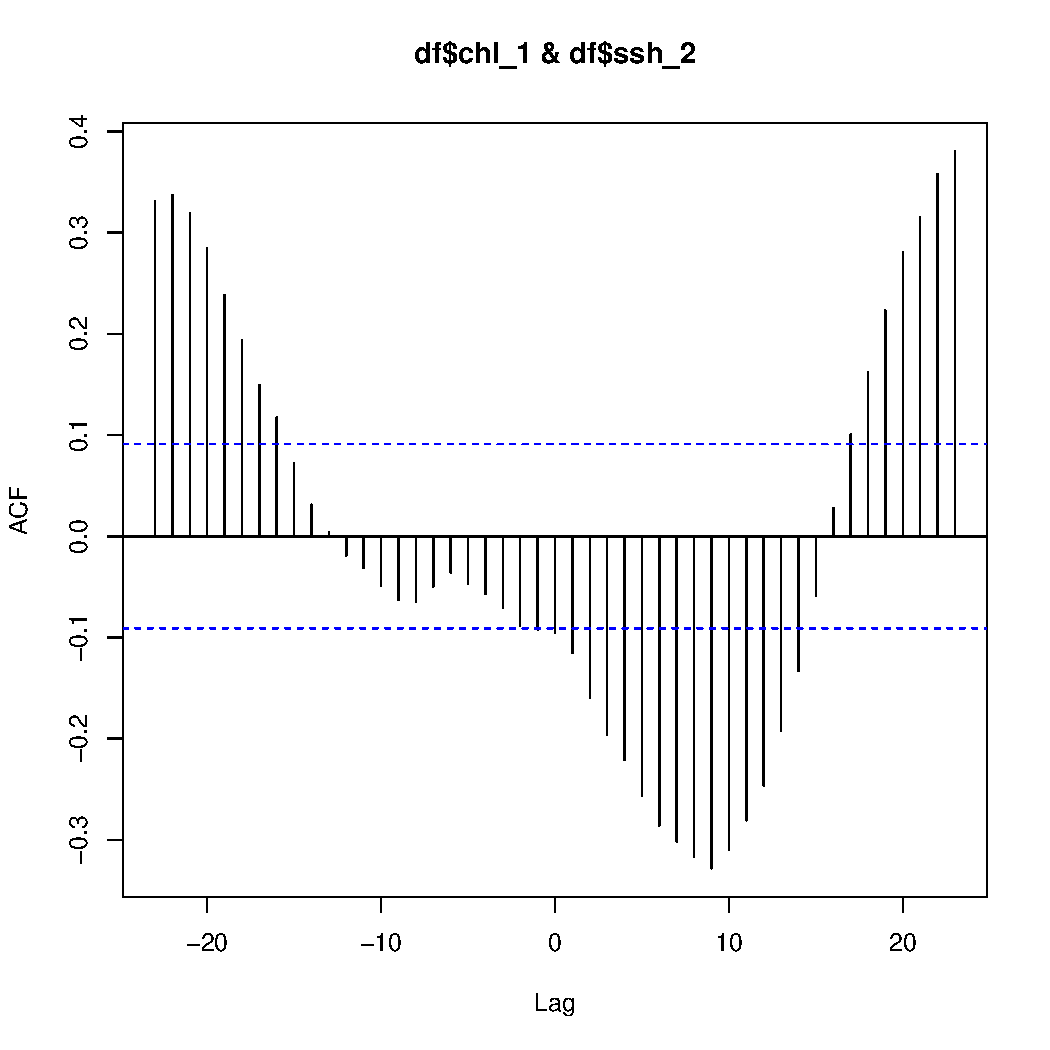
\includegraphics[width=\maxwidth]{figure/unnamed-chunk-12-2} 

\end{knitrout}

\begin{knitrout}
\definecolor{shadecolor}{rgb}{0.969, 0.969, 0.969}\color{fgcolor}\begin{kframe}
\begin{alltt}
\hlkwd{qplot}\hlstd{(chl_1, ssh_3,} \hlkwc{data}\hlstd{=df,} \hlkwc{geom}\hlstd{=}\hlkwd{c}\hlstd{(}\hlstr{'point'}\hlstd{,} \hlstr{'smooth'}\hlstd{),} \hlkwc{method}\hlstd{=}\hlstr{'lm'}\hlstd{,} \hlkwc{formula}\hlstd{=y}\hlopt{~}\hlstd{x)}
\end{alltt}
\end{kframe}
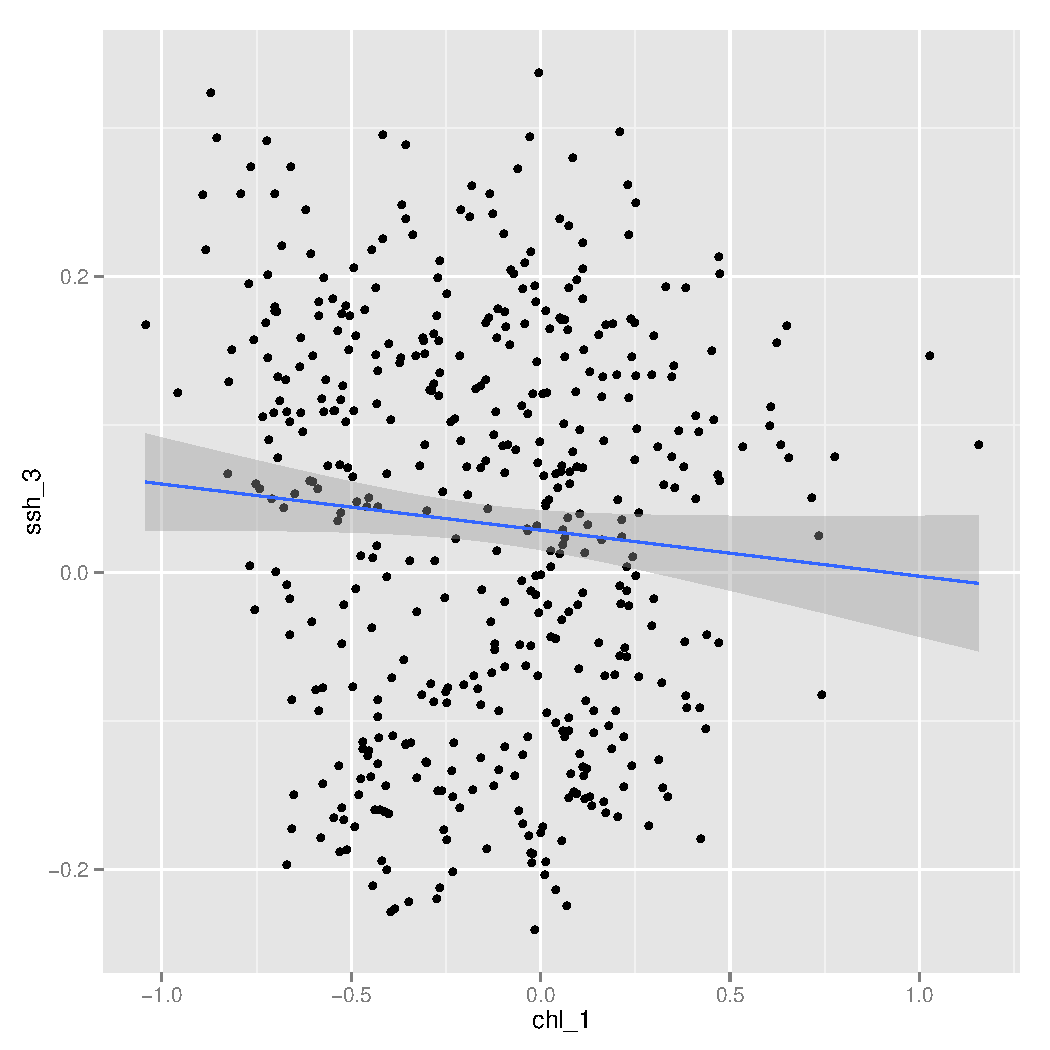
\includegraphics[width=\maxwidth]{figure/unnamed-chunk-13-1} 
\begin{kframe}\begin{alltt}
\hlcom{## Correlation coefficient}
\hlkwd{cor}\hlstd{(df}\hlopt{$}\hlstd{chl_1, df}\hlopt{$}\hlstd{ssh_3,} \hlkwc{use}\hlstd{=}\hlstr{'complete.obs'}\hlstd{)}
\end{alltt}
\begin{verbatim}
## [1] -0.08408265
\end{verbatim}
\begin{alltt}
\hlkwd{ccf}\hlstd{(df}\hlopt{$}\hlstd{chl_1, df}\hlopt{$}\hlstd{ssh_3,} \hlkwc{na.action}\hlstd{=na.pass)}
\end{alltt}
\end{kframe}
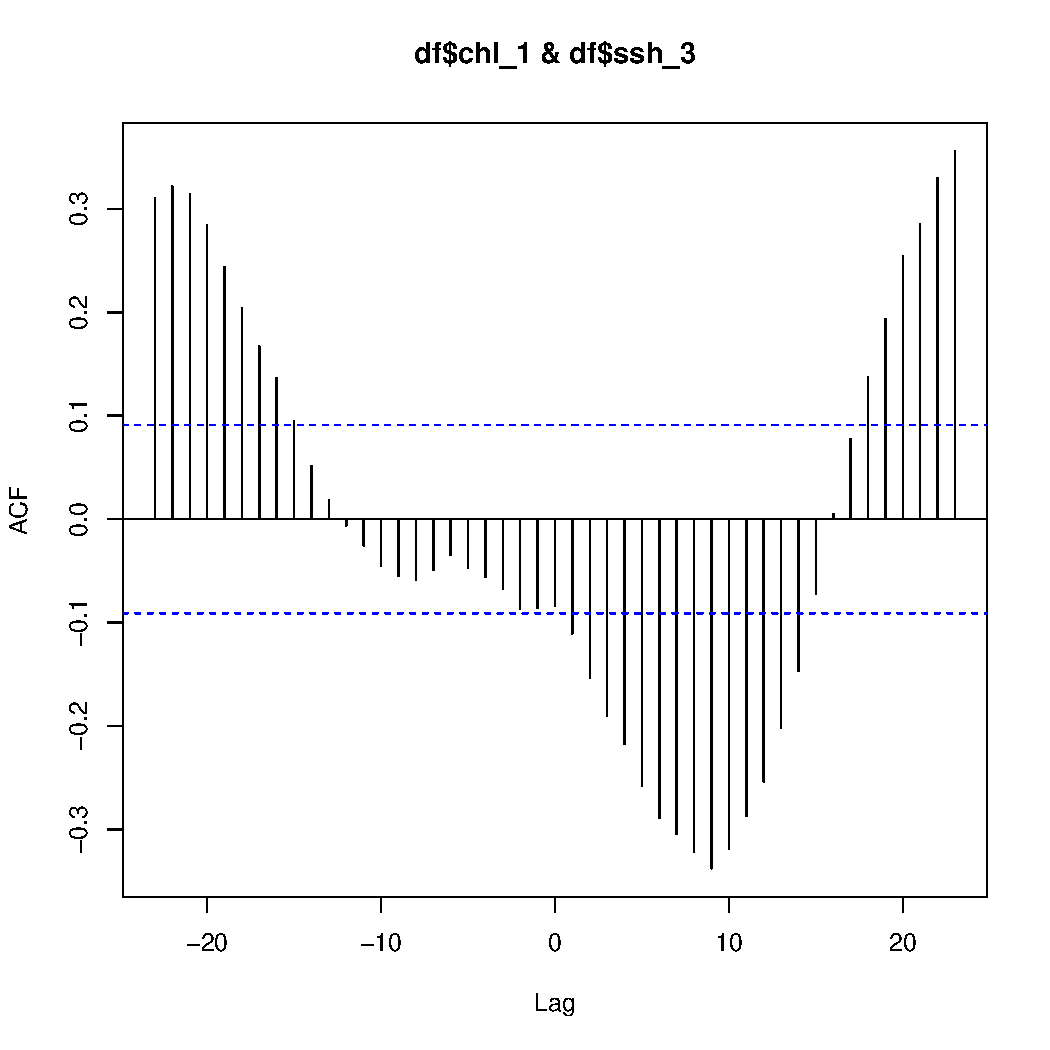
\includegraphics[width=\maxwidth]{figure/unnamed-chunk-13-2} 

\end{knitrout}

\begin{knitrout}
\definecolor{shadecolor}{rgb}{0.969, 0.969, 0.969}\color{fgcolor}\begin{kframe}
\begin{alltt}
\hlkwd{qplot}\hlstd{(chl_1, ssh_4,} \hlkwc{data}\hlstd{=df,} \hlkwc{geom}\hlstd{=}\hlkwd{c}\hlstd{(}\hlstr{'point'}\hlstd{,} \hlstr{'smooth'}\hlstd{),} \hlkwc{method}\hlstd{=}\hlstr{'lm'}\hlstd{,} \hlkwc{formula}\hlstd{=y}\hlopt{~}\hlstd{x)}
\end{alltt}
\end{kframe}
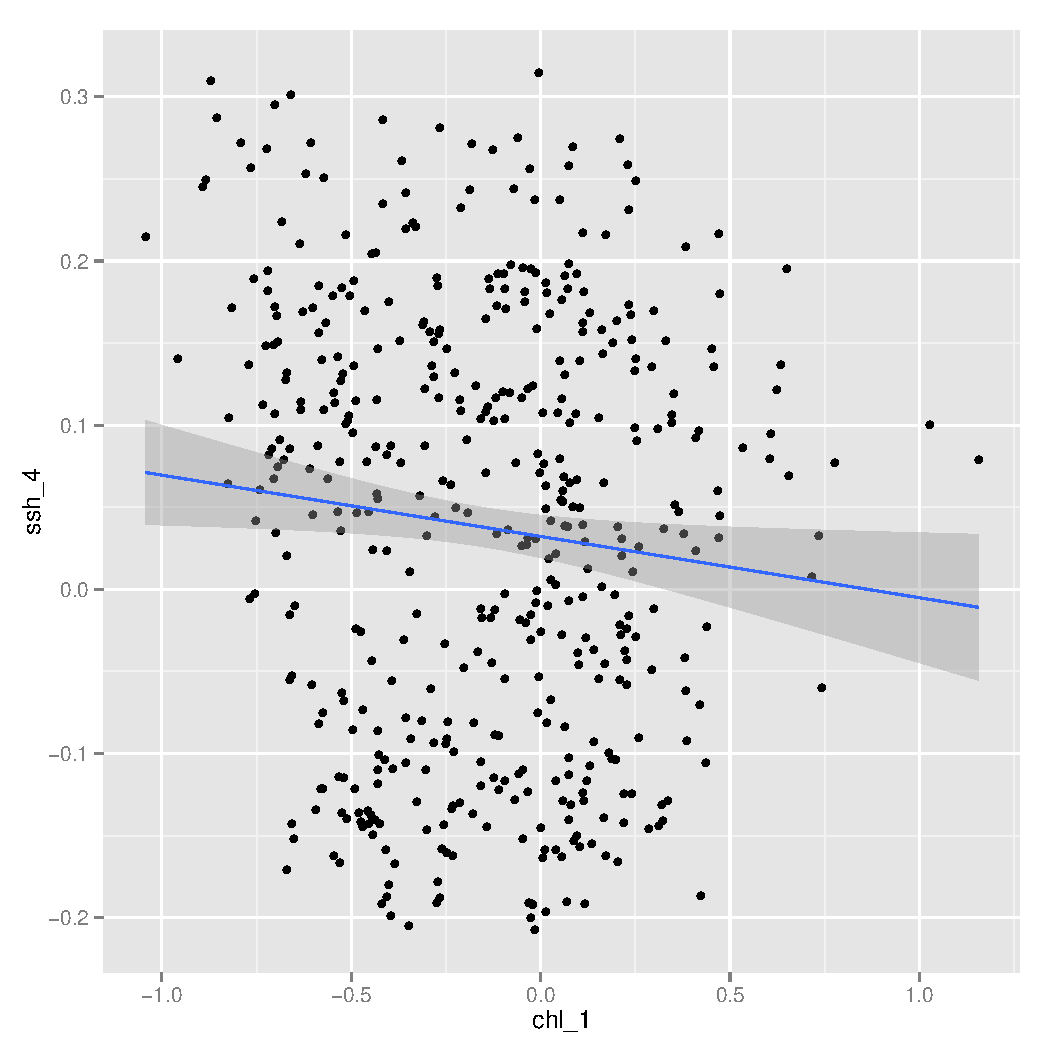
\includegraphics[width=\maxwidth]{figure/unnamed-chunk-14-1} 
\begin{kframe}\begin{alltt}
\hlcom{## Correlation coefficient}
\hlkwd{cor}\hlstd{(df}\hlopt{$}\hlstd{chl_1, df}\hlopt{$}\hlstd{ssh_4,} \hlkwc{use}\hlstd{=}\hlstr{'complete.obs'}\hlstd{)}
\end{alltt}
\begin{verbatim}
## [1] -0.1034069
\end{verbatim}
\begin{alltt}
\hlkwd{ccf}\hlstd{(df}\hlopt{$}\hlstd{chl_1, df}\hlopt{$}\hlstd{ssh_4,} \hlkwc{na.action}\hlstd{=na.pass)}
\end{alltt}
\end{kframe}
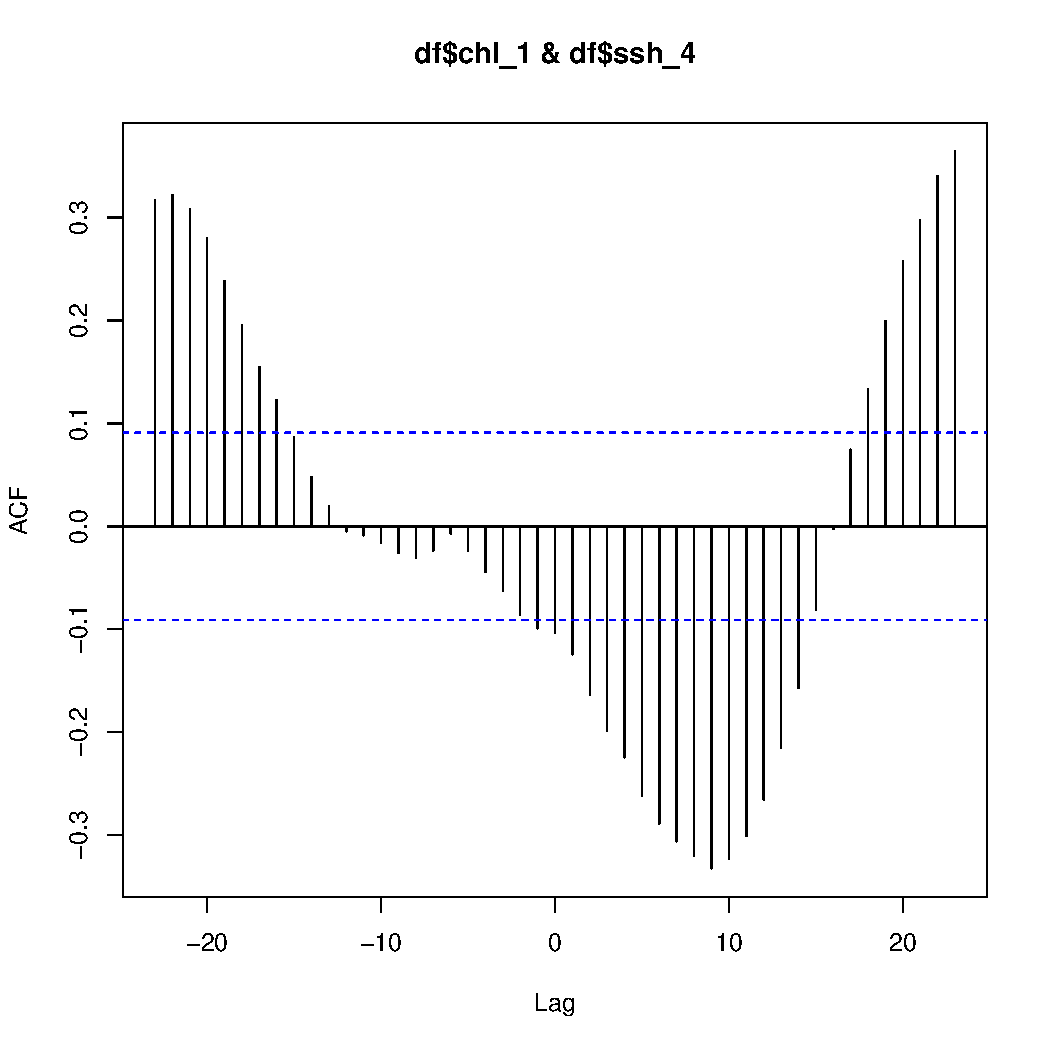
\includegraphics[width=\maxwidth]{figure/unnamed-chunk-14-2} 

\end{knitrout}

\subsection{Chlorophyll and PAR}

\begin{knitrout}
\definecolor{shadecolor}{rgb}{0.969, 0.969, 0.969}\color{fgcolor}\begin{kframe}
\begin{alltt}
\hlkwd{qplot}\hlstd{(chl_1, par_1,} \hlkwc{data}\hlstd{=df,} \hlkwc{geom}\hlstd{=}\hlkwd{c}\hlstd{(}\hlstr{'point'}\hlstd{,} \hlstr{'smooth'}\hlstd{),} \hlkwc{method}\hlstd{=}\hlstr{'lm'}\hlstd{,} \hlkwc{formula}\hlstd{=y}\hlopt{~}\hlstd{x)}
\end{alltt}
\end{kframe}
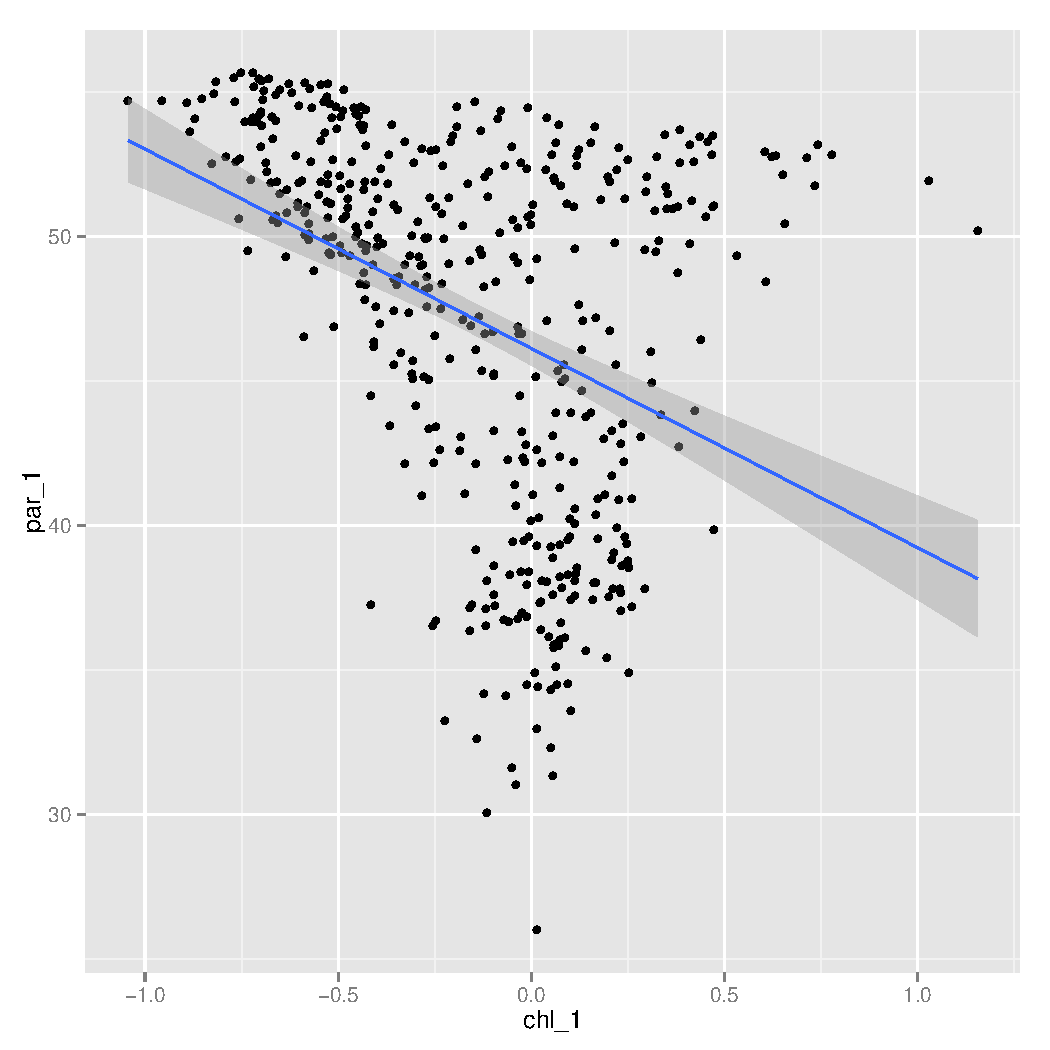
\includegraphics[width=\maxwidth]{figure/unnamed-chunk-15-1} 
\begin{kframe}\begin{alltt}
\hlcom{## Correlation coefficient}
\hlkwd{cor}\hlstd{(df}\hlopt{$}\hlstd{chl_1, df}\hlopt{$}\hlstd{par_1,} \hlkwc{use}\hlstd{=}\hlstr{'complete.obs'}\hlstd{)}
\end{alltt}
\begin{verbatim}
## [1] -0.3894663
\end{verbatim}
\begin{alltt}
\hlkwd{ccf}\hlstd{(df}\hlopt{$}\hlstd{chl_1, df}\hlopt{$}\hlstd{par_1,} \hlkwc{na.action}\hlstd{=na.pass)}
\end{alltt}
\end{kframe}
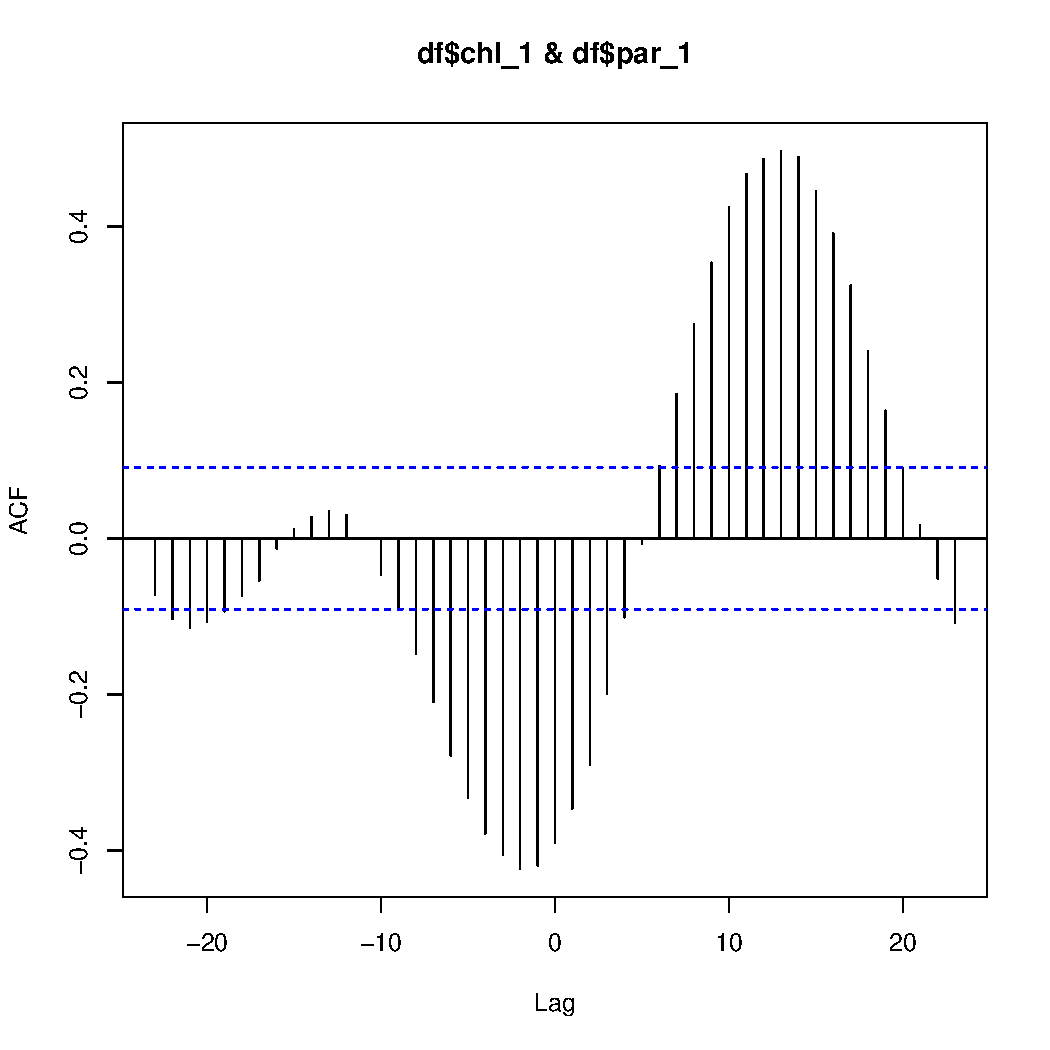
\includegraphics[width=\maxwidth]{figure/unnamed-chunk-15-2} 

\end{knitrout}

\begin{knitrout}
\definecolor{shadecolor}{rgb}{0.969, 0.969, 0.969}\color{fgcolor}\begin{kframe}
\begin{alltt}
\hlkwd{qplot}\hlstd{(chl_1, par_2,} \hlkwc{data}\hlstd{=df,} \hlkwc{geom}\hlstd{=}\hlkwd{c}\hlstd{(}\hlstr{'point'}\hlstd{,} \hlstr{'smooth'}\hlstd{),} \hlkwc{method}\hlstd{=}\hlstr{'lm'}\hlstd{,} \hlkwc{formula}\hlstd{=y}\hlopt{~}\hlstd{x)}
\end{alltt}
\end{kframe}
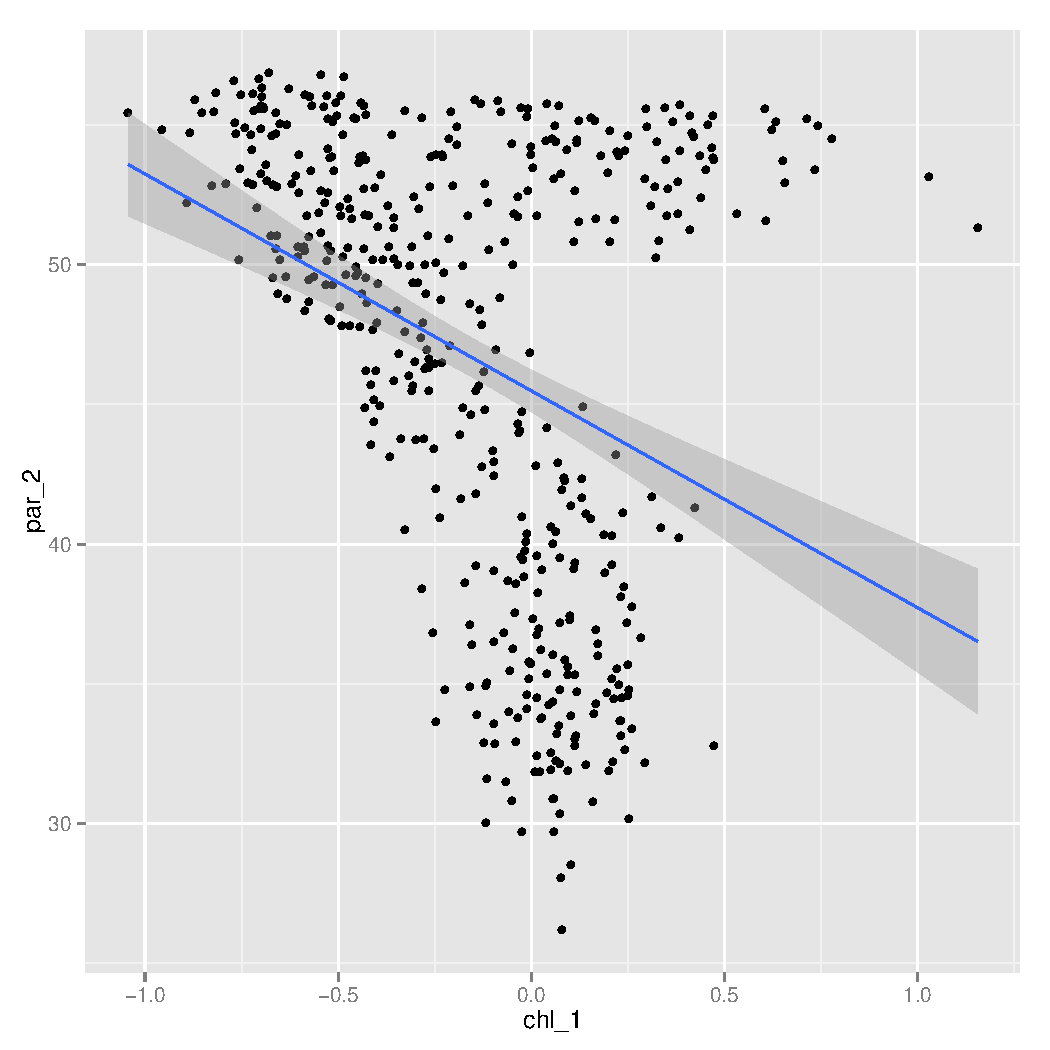
\includegraphics[width=\maxwidth]{figure/unnamed-chunk-16-1} 
\begin{kframe}\begin{alltt}
\hlcom{## Correlation coefficient}
\hlkwd{cor}\hlstd{(df}\hlopt{$}\hlstd{chl_1, df}\hlopt{$}\hlstd{par_2,} \hlkwc{use}\hlstd{=}\hlstr{'complete.obs'}\hlstd{)}
\end{alltt}
\begin{verbatim}
## [1] -0.3482226
\end{verbatim}
\begin{alltt}
\hlkwd{ccf}\hlstd{(df}\hlopt{$}\hlstd{chl_1, df}\hlopt{$}\hlstd{par_2,} \hlkwc{na.action}\hlstd{=na.pass)}
\end{alltt}
\end{kframe}
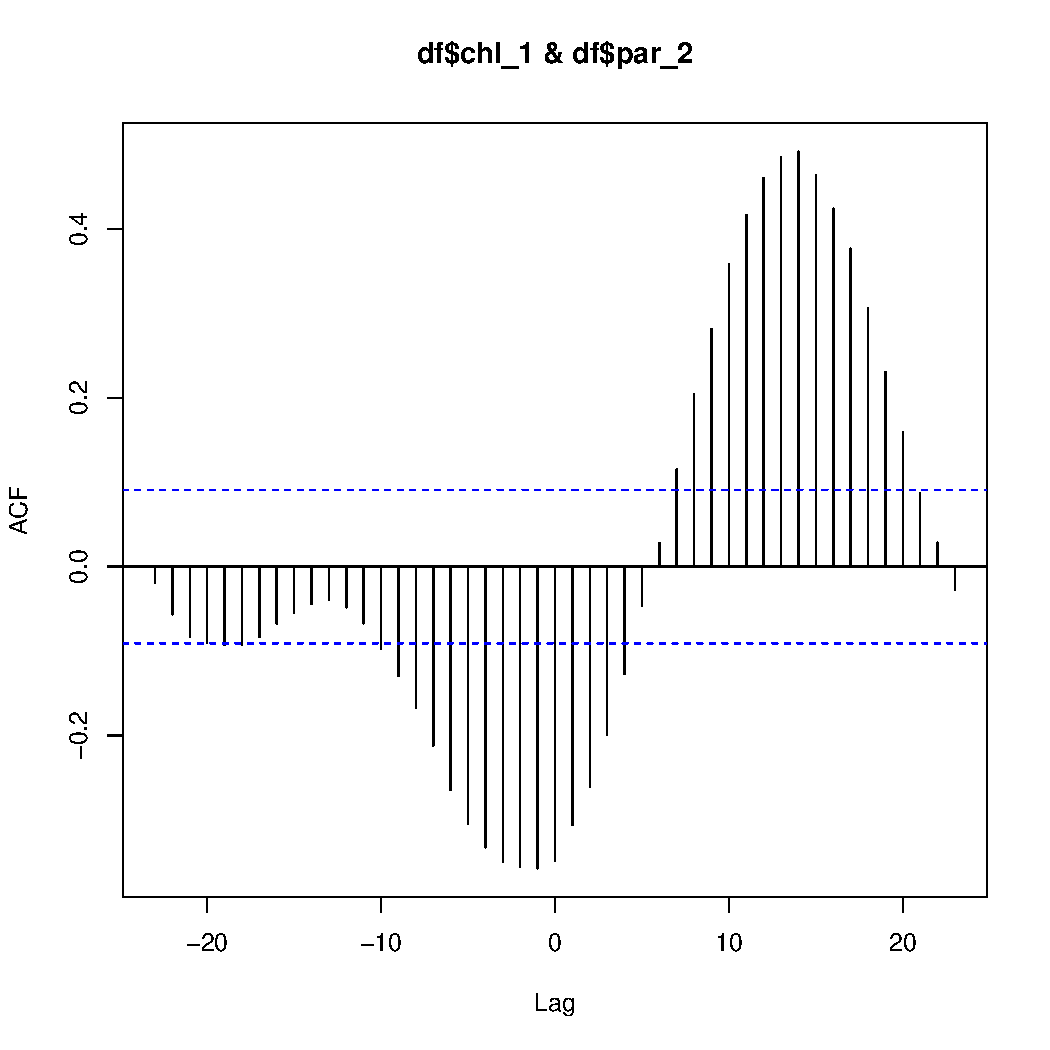
\includegraphics[width=\maxwidth]{figure/unnamed-chunk-16-2} 

\end{knitrout}

\begin{knitrout}
\definecolor{shadecolor}{rgb}{0.969, 0.969, 0.969}\color{fgcolor}\begin{kframe}
\begin{alltt}
\hlkwd{qplot}\hlstd{(chl_1, par_3,} \hlkwc{data}\hlstd{=df,} \hlkwc{geom}\hlstd{=}\hlkwd{c}\hlstd{(}\hlstr{'point'}\hlstd{,} \hlstr{'smooth'}\hlstd{),} \hlkwc{method}\hlstd{=}\hlstr{'lm'}\hlstd{,} \hlkwc{formula}\hlstd{=y}\hlopt{~}\hlstd{x)}
\end{alltt}
\end{kframe}
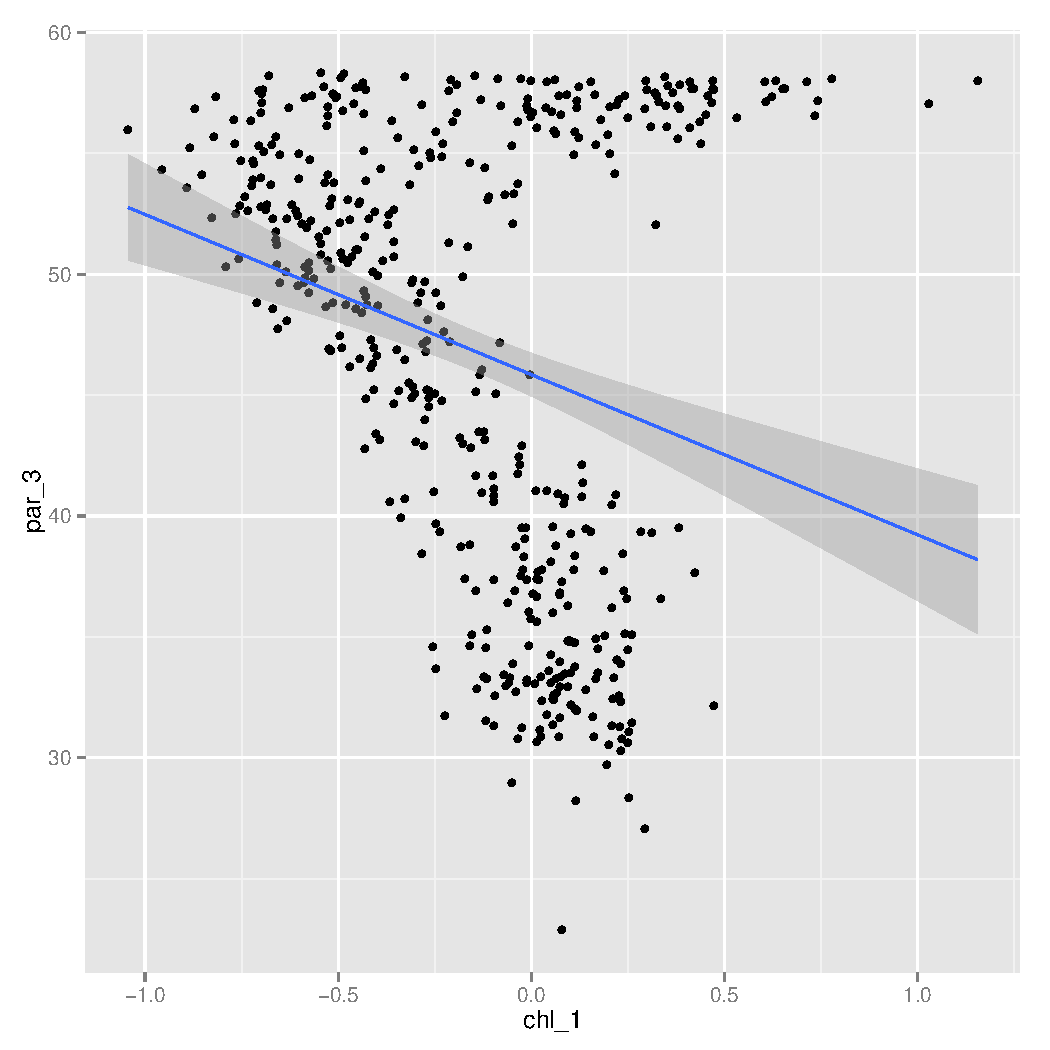
\includegraphics[width=\maxwidth]{figure/unnamed-chunk-17-1} 
\begin{kframe}\begin{alltt}
\hlcom{## Correlation coefficient}
\hlkwd{cor}\hlstd{(df}\hlopt{$}\hlstd{chl_1, df}\hlopt{$}\hlstd{par_3,} \hlkwc{use}\hlstd{=}\hlstr{'complete.obs'}\hlstd{)}
\end{alltt}
\begin{verbatim}
## [1] -0.2584293
\end{verbatim}
\begin{alltt}
\hlkwd{ccf}\hlstd{(df}\hlopt{$}\hlstd{chl_1, df}\hlopt{$}\hlstd{par_3,} \hlkwc{na.action}\hlstd{=na.pass)}
\end{alltt}
\end{kframe}
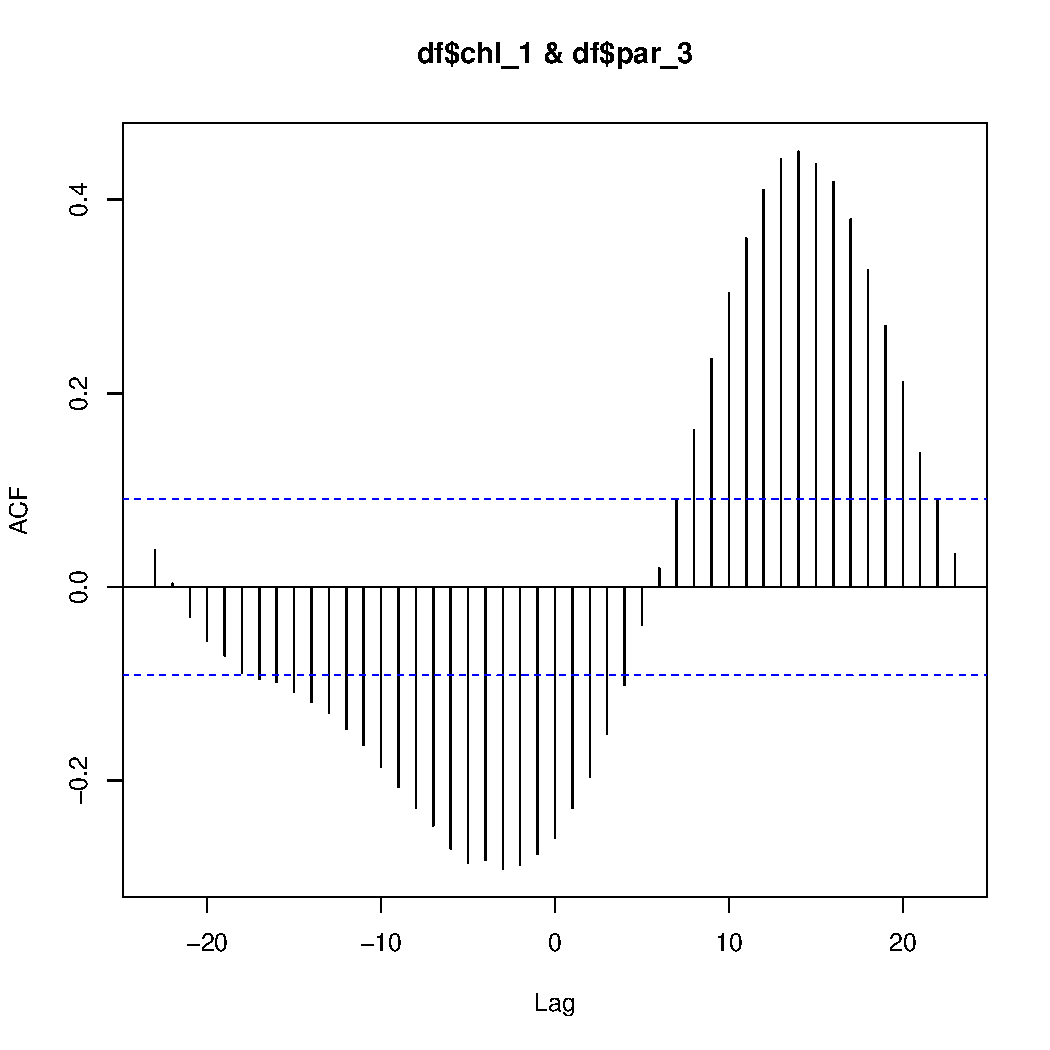
\includegraphics[width=\maxwidth]{figure/unnamed-chunk-17-2} 

\end{knitrout}

\begin{knitrout}
\definecolor{shadecolor}{rgb}{0.969, 0.969, 0.969}\color{fgcolor}\begin{kframe}
\begin{alltt}
\hlkwd{qplot}\hlstd{(chl_1, par_4,} \hlkwc{data}\hlstd{=df,} \hlkwc{geom}\hlstd{=}\hlkwd{c}\hlstd{(}\hlstr{'point'}\hlstd{,} \hlstr{'smooth'}\hlstd{),} \hlkwc{method}\hlstd{=}\hlstr{'lm'}\hlstd{,} \hlkwc{formula}\hlstd{=y}\hlopt{~}\hlstd{x)}
\end{alltt}
\end{kframe}
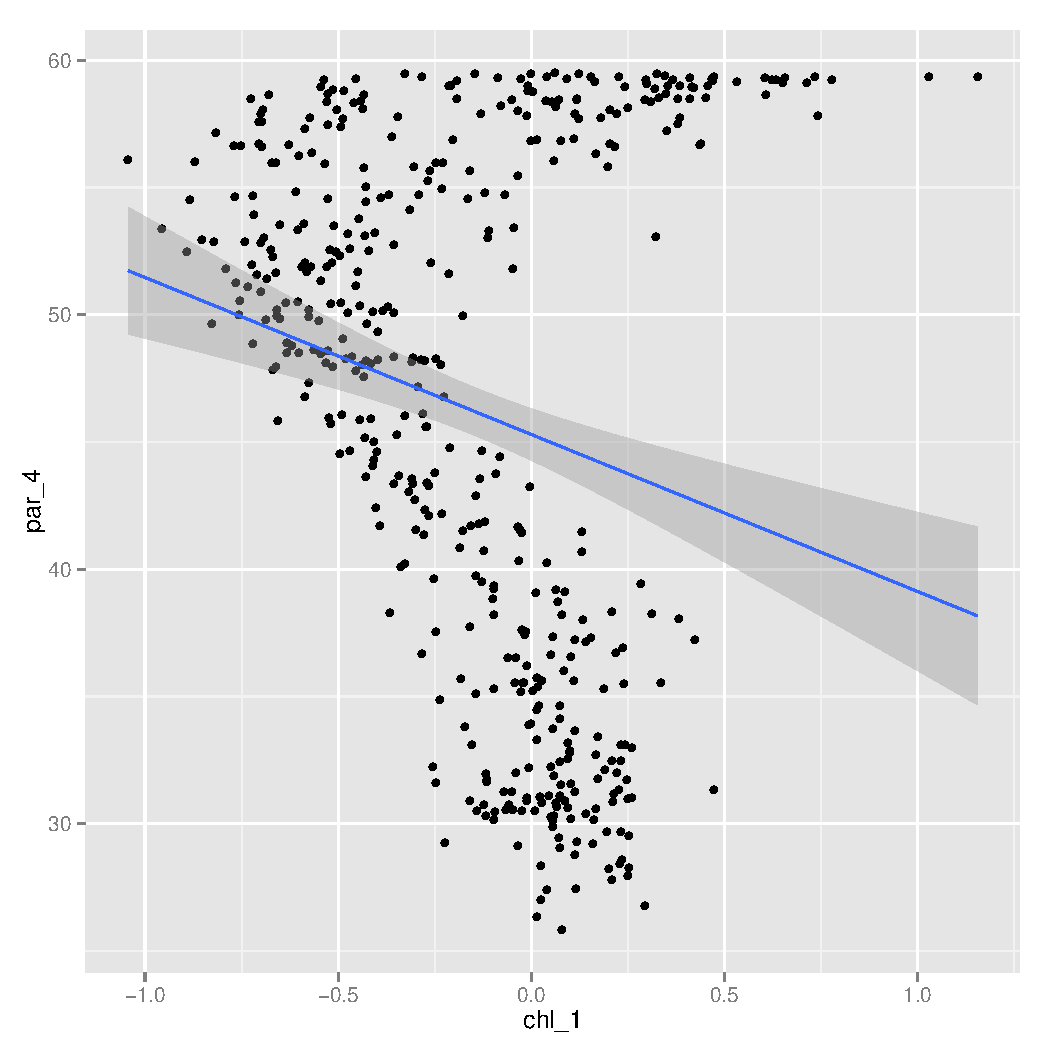
\includegraphics[width=\maxwidth]{figure/unnamed-chunk-18-1} 
\begin{kframe}\begin{alltt}
\hlcom{## Correlation coefficient}
\hlkwd{cor}\hlstd{(df}\hlopt{$}\hlstd{chl_1, df}\hlopt{$}\hlstd{par_4,} \hlkwc{use}\hlstd{=}\hlstr{'complete.obs'}\hlstd{)}
\end{alltt}
\begin{verbatim}
## [1] -0.213377
\end{verbatim}
\begin{alltt}
\hlkwd{ccf}\hlstd{(df}\hlopt{$}\hlstd{chl_1, df}\hlopt{$}\hlstd{par_4,} \hlkwc{na.action}\hlstd{=na.pass)}
\end{alltt}
\end{kframe}
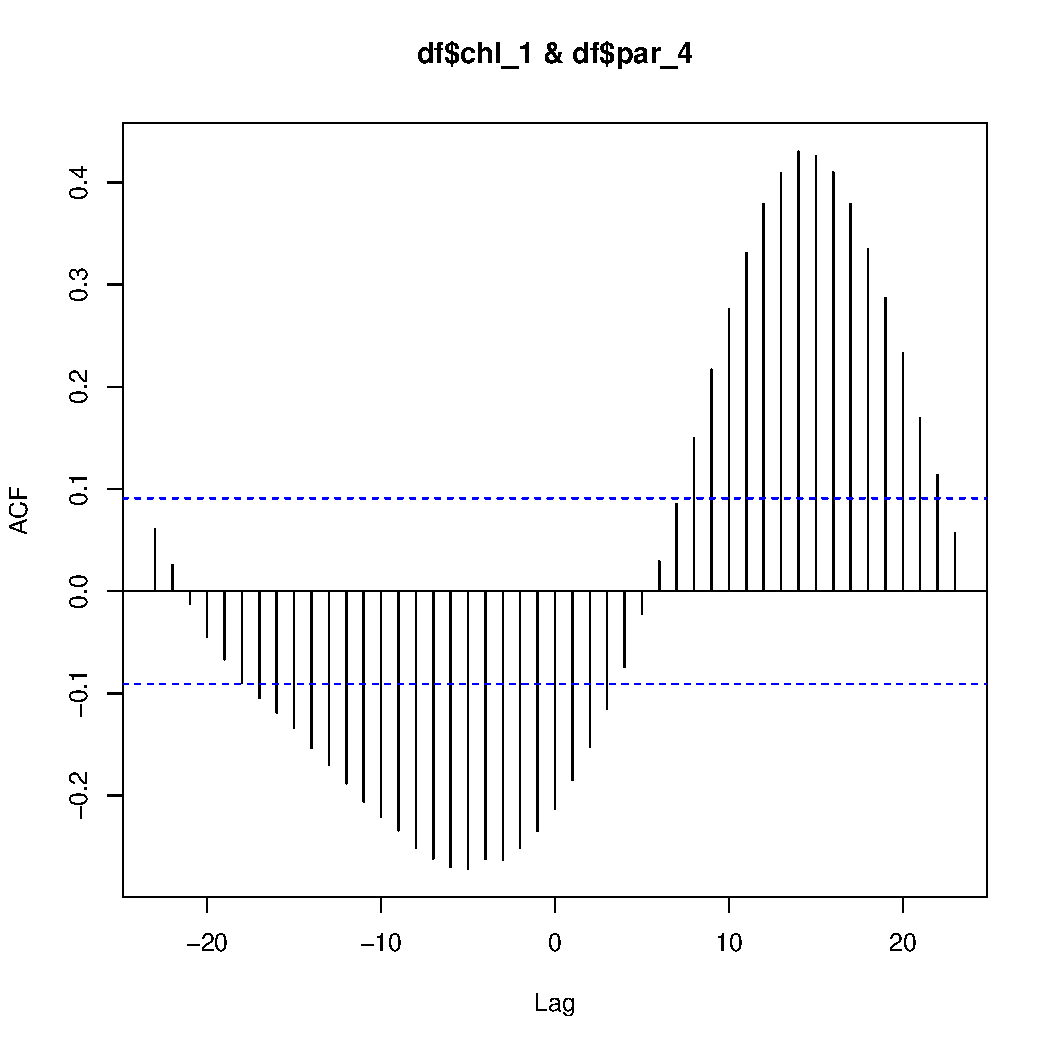
\includegraphics[width=\maxwidth]{figure/unnamed-chunk-18-2} 

\end{knitrout}

\subsection{Chlorophyll and AOT}

\begin{knitrout}
\definecolor{shadecolor}{rgb}{0.969, 0.969, 0.969}\color{fgcolor}\begin{kframe}
\begin{alltt}
\hlkwd{qplot}\hlstd{(chl_1, aot_1,} \hlkwc{data}\hlstd{=df,} \hlkwc{geom}\hlstd{=}\hlkwd{c}\hlstd{(}\hlstr{'point'}\hlstd{,} \hlstr{'smooth'}\hlstd{),} \hlkwc{method}\hlstd{=}\hlstr{'lm'}\hlstd{,} \hlkwc{formula}\hlstd{=y}\hlopt{~}\hlstd{x)}
\end{alltt}


{\ttfamily\noindent\color{warningcolor}{\#\# Warning: Removed 90 rows containing missing values (stat\_smooth).}}

{\ttfamily\noindent\color{warningcolor}{\#\# Warning: Removed 90 rows containing missing values (geom\_point).}}\end{kframe}
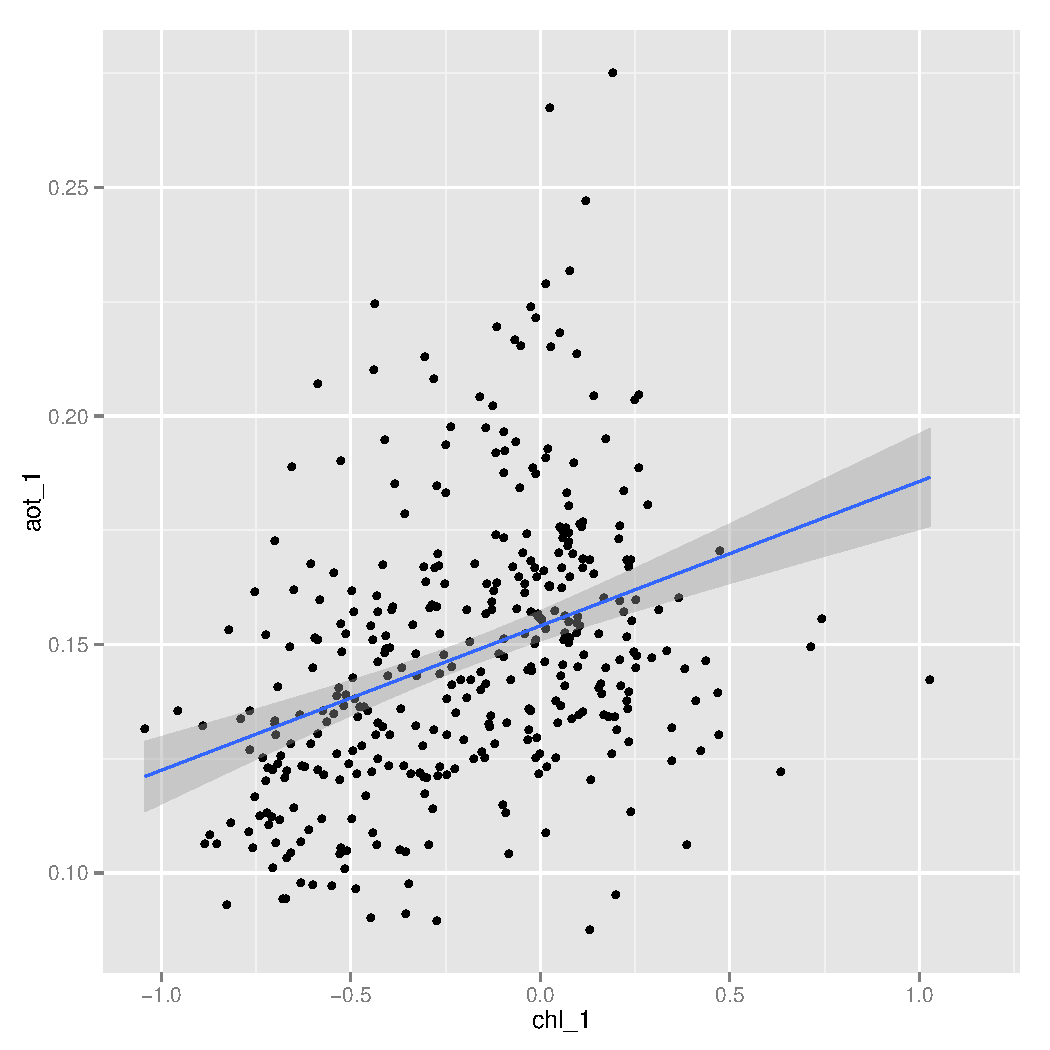
\includegraphics[width=\maxwidth]{figure/unnamed-chunk-19-1} 
\begin{kframe}\begin{alltt}
\hlcom{## Correlation coefficient}
\hlkwd{cor}\hlstd{(df}\hlopt{$}\hlstd{chl_1, df}\hlopt{$}\hlstd{aot_1,} \hlkwc{use}\hlstd{=}\hlstr{'complete.obs'}\hlstd{)}
\end{alltt}
\begin{verbatim}
## [1] 0.3559261
\end{verbatim}
\begin{alltt}
\hlkwd{ccf}\hlstd{(df}\hlopt{$}\hlstd{chl_1, df}\hlopt{$}\hlstd{aot_1,} \hlkwc{na.action}\hlstd{=na.pass)}
\end{alltt}
\end{kframe}
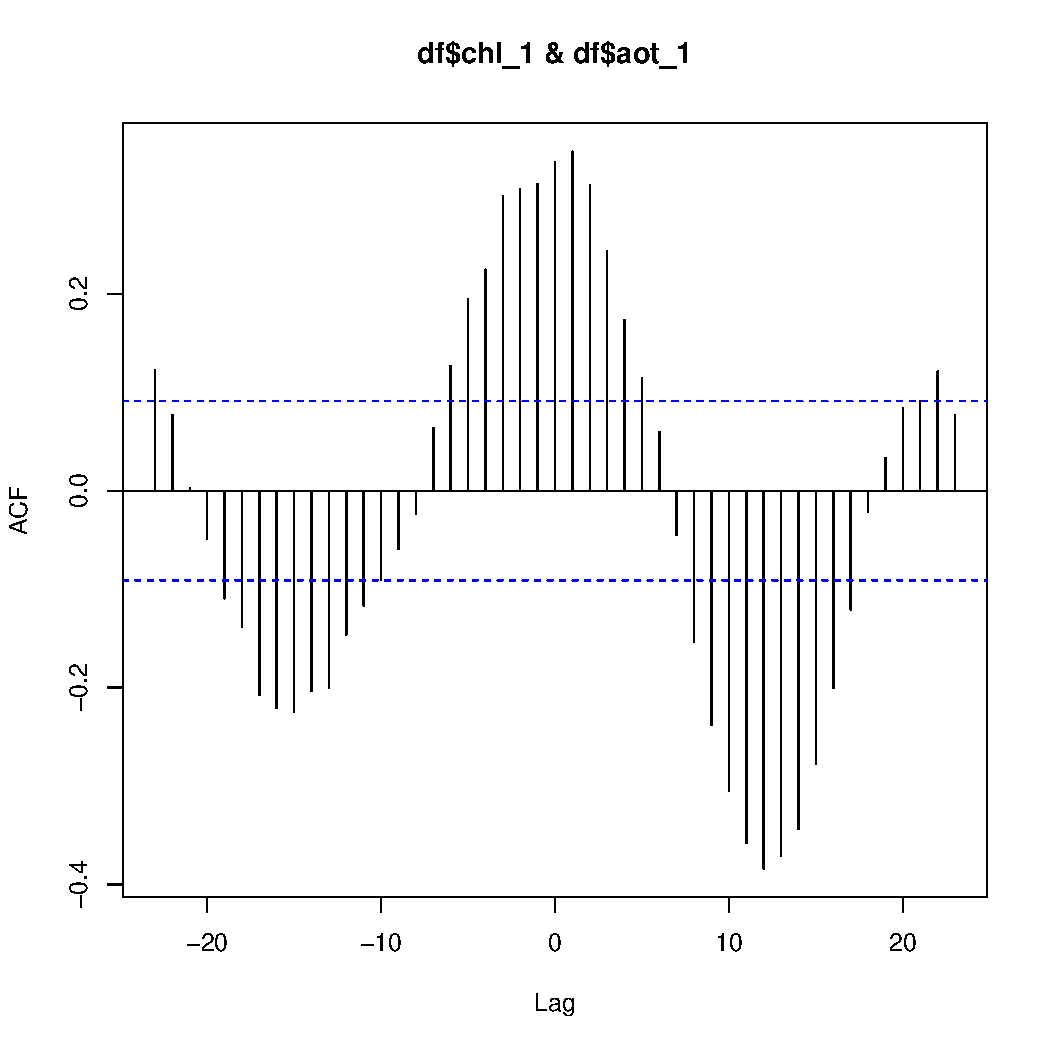
\includegraphics[width=\maxwidth]{figure/unnamed-chunk-19-2} 

\end{knitrout}

\begin{knitrout}
\definecolor{shadecolor}{rgb}{0.969, 0.969, 0.969}\color{fgcolor}\begin{kframe}
\begin{alltt}
\hlkwd{qplot}\hlstd{(chl_1, aot_2,} \hlkwc{data}\hlstd{=df,} \hlkwc{geom}\hlstd{=}\hlkwd{c}\hlstd{(}\hlstr{'point'}\hlstd{,} \hlstr{'smooth'}\hlstd{),} \hlkwc{method}\hlstd{=}\hlstr{'lm'}\hlstd{,} \hlkwc{formula}\hlstd{=y}\hlopt{~}\hlstd{x)}
\end{alltt}


{\ttfamily\noindent\color{warningcolor}{\#\# Warning: Removed 62 rows containing missing values (stat\_smooth).}}

{\ttfamily\noindent\color{warningcolor}{\#\# Warning: Removed 62 rows containing missing values (geom\_point).}}\end{kframe}
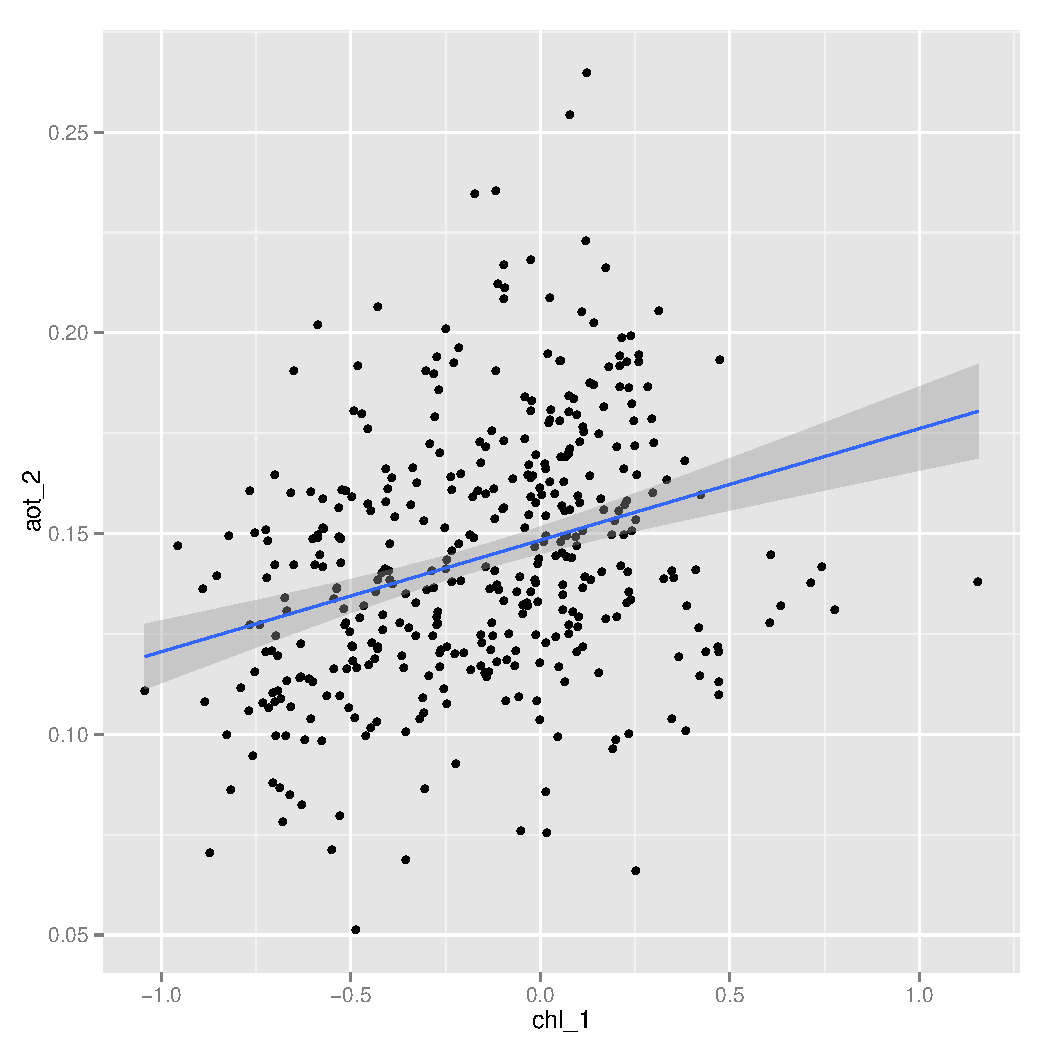
\includegraphics[width=\maxwidth]{figure/unnamed-chunk-20-1} 
\begin{kframe}\begin{alltt}
\hlcom{## Correlation coefficient}
\hlkwd{cor}\hlstd{(df}\hlopt{$}\hlstd{chl_1, df}\hlopt{$}\hlstd{aot_2,} \hlkwc{use}\hlstd{=}\hlstr{'complete.obs'}\hlstd{)}
\end{alltt}
\begin{verbatim}
## [1] 0.3044926
\end{verbatim}
\begin{alltt}
\hlkwd{ccf}\hlstd{(df}\hlopt{$}\hlstd{chl_1, df}\hlopt{$}\hlstd{aot_2,} \hlkwc{na.action}\hlstd{=na.pass)}
\end{alltt}
\end{kframe}
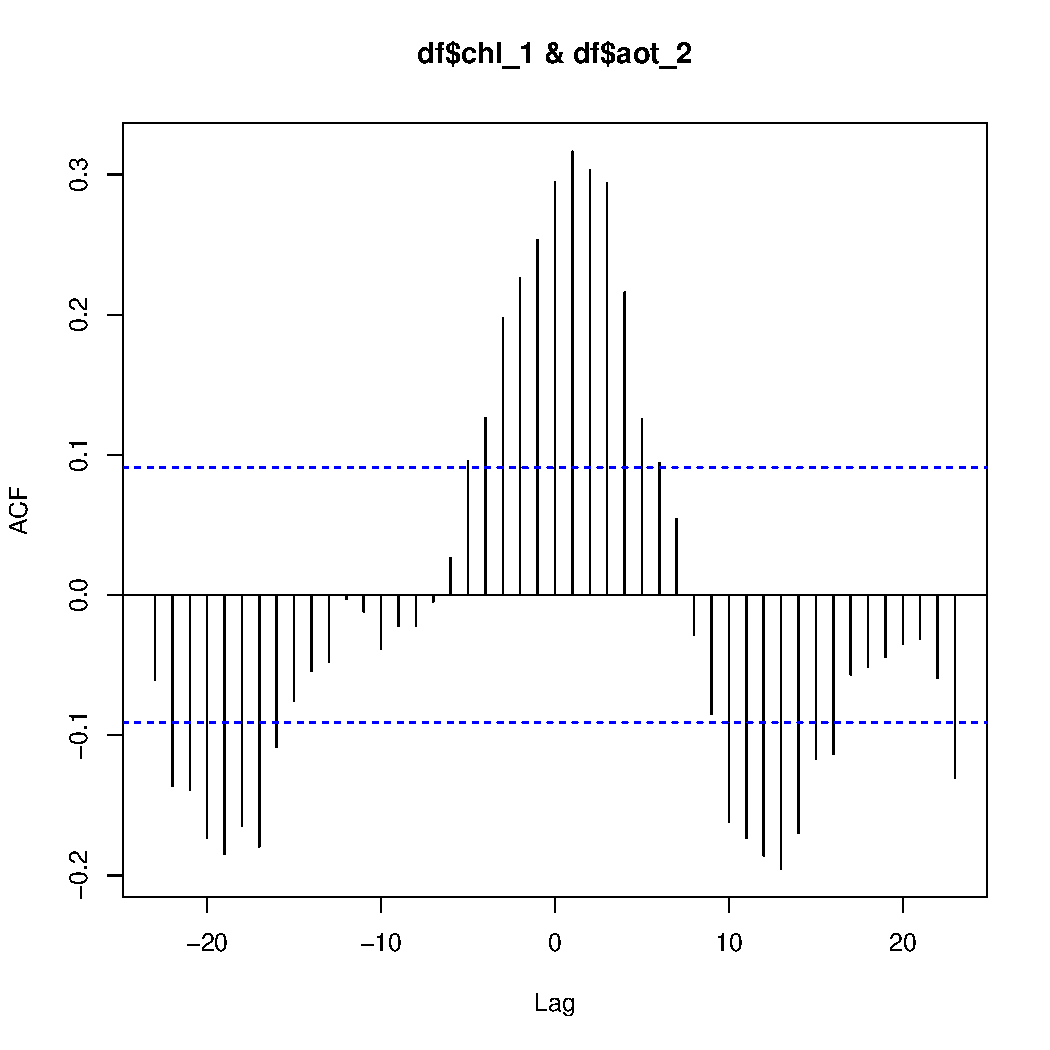
\includegraphics[width=\maxwidth]{figure/unnamed-chunk-20-2} 

\end{knitrout}

\begin{knitrout}
\definecolor{shadecolor}{rgb}{0.969, 0.969, 0.969}\color{fgcolor}\begin{kframe}
\begin{alltt}
\hlkwd{qplot}\hlstd{(chl_1, aot_3,} \hlkwc{data}\hlstd{=df,} \hlkwc{geom}\hlstd{=}\hlkwd{c}\hlstd{(}\hlstr{'point'}\hlstd{,} \hlstr{'smooth'}\hlstd{),} \hlkwc{method}\hlstd{=}\hlstr{'lm'}\hlstd{,} \hlkwc{formula}\hlstd{=y}\hlopt{~}\hlstd{x)}
\end{alltt}


{\ttfamily\noindent\color{warningcolor}{\#\# Warning: Removed 9 rows containing missing values (stat\_smooth).}}

{\ttfamily\noindent\color{warningcolor}{\#\# Warning: Removed 9 rows containing missing values (geom\_point).}}\end{kframe}
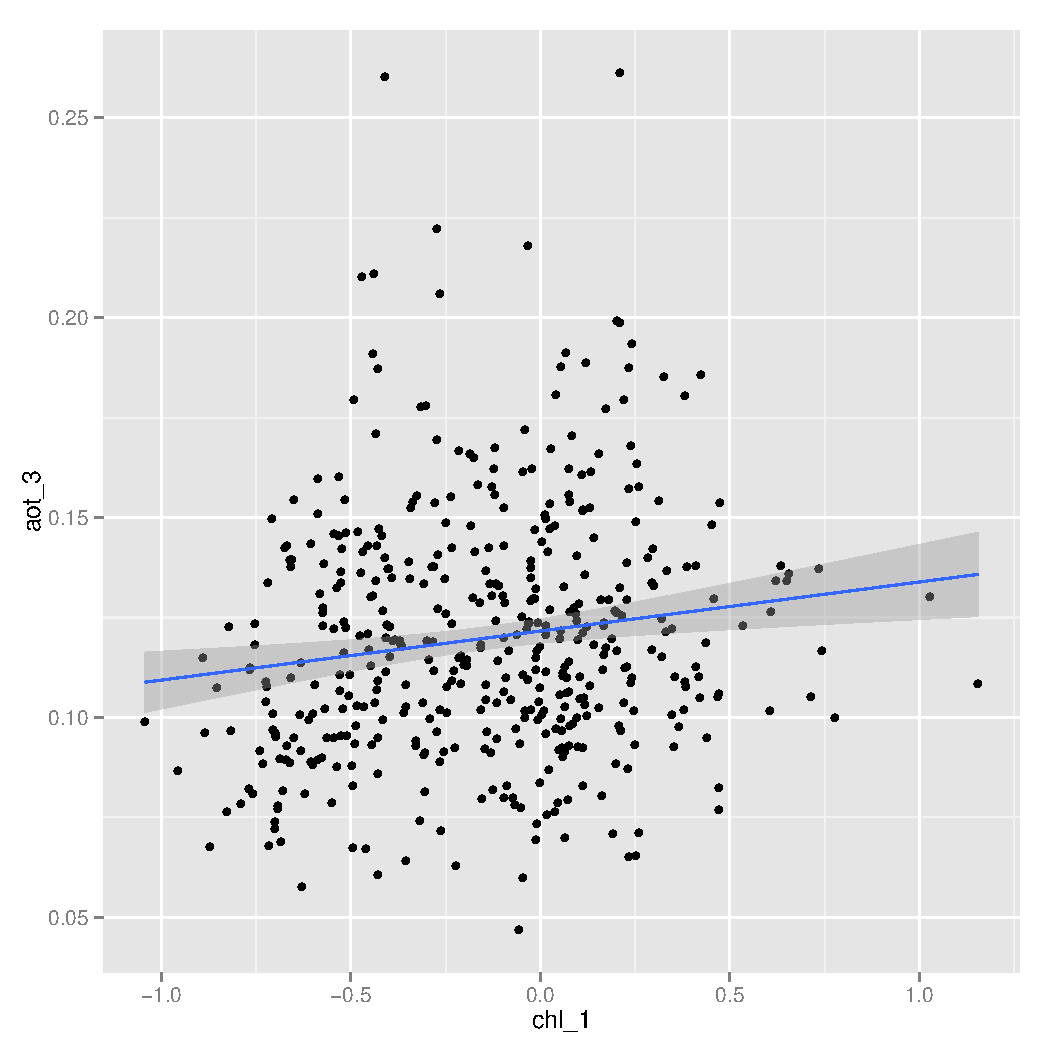
\includegraphics[width=\maxwidth]{figure/unnamed-chunk-21-1} 
\begin{kframe}\begin{alltt}
\hlcom{## Correlation coefficient}
\hlkwd{cor}\hlstd{(df}\hlopt{$}\hlstd{chl_1, df}\hlopt{$}\hlstd{aot_3,} \hlkwc{use}\hlstd{=}\hlstr{'complete.obs'}\hlstd{)}
\end{alltt}
\begin{verbatim}
## [1] 0.1435728
\end{verbatim}
\begin{alltt}
\hlkwd{ccf}\hlstd{(df}\hlopt{$}\hlstd{chl_1, df}\hlopt{$}\hlstd{aot_3,} \hlkwc{na.action}\hlstd{=na.pass)}
\end{alltt}
\end{kframe}
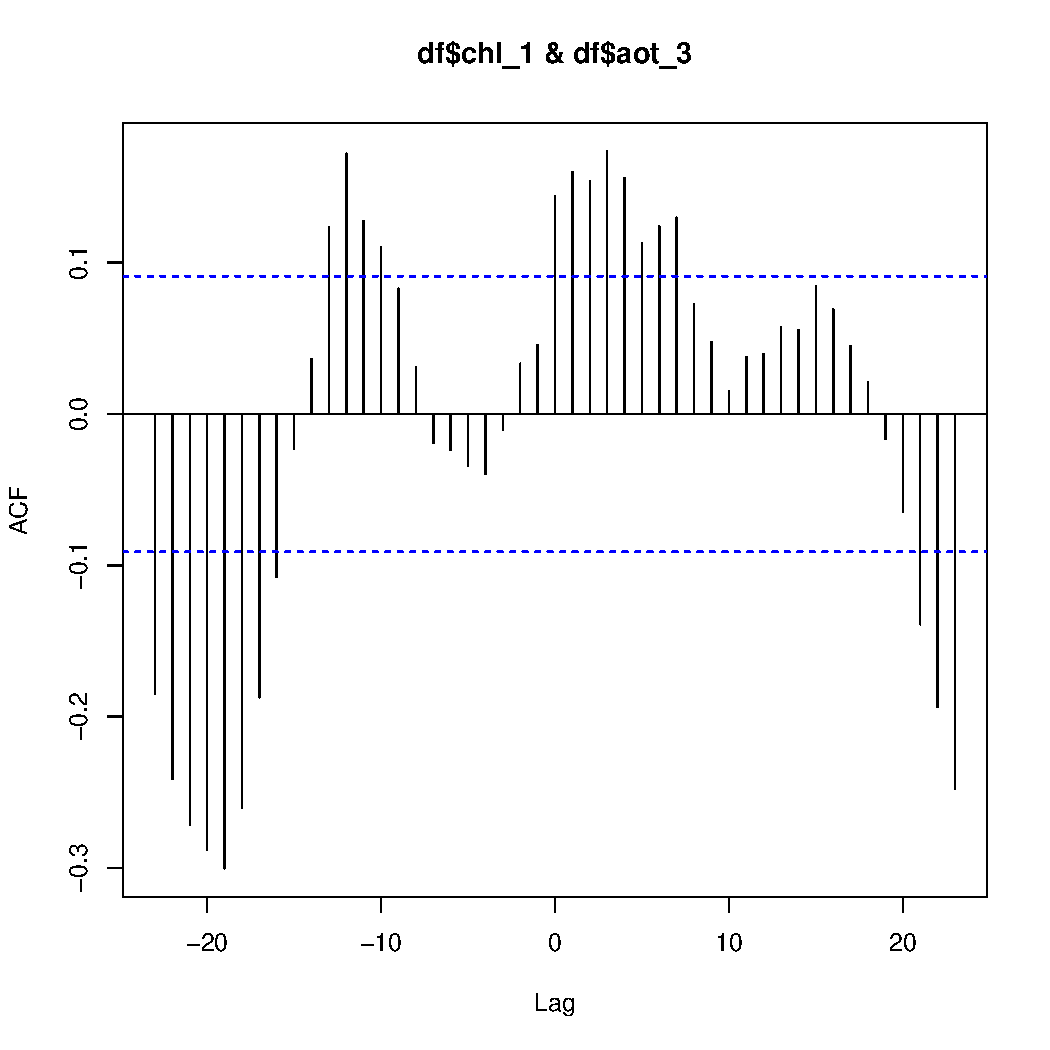
\includegraphics[width=\maxwidth]{figure/unnamed-chunk-21-2} 

\end{knitrout}

\begin{knitrout}
\definecolor{shadecolor}{rgb}{0.969, 0.969, 0.969}\color{fgcolor}\begin{kframe}
\begin{alltt}
\hlkwd{qplot}\hlstd{(chl_1, aot_4,} \hlkwc{data}\hlstd{=df,} \hlkwc{geom}\hlstd{=}\hlkwd{c}\hlstd{(}\hlstr{'point'}\hlstd{,} \hlstr{'smooth'}\hlstd{),} \hlkwc{method}\hlstd{=}\hlstr{'lm'}\hlstd{,} \hlkwc{formula}\hlstd{=y}\hlopt{~}\hlstd{x)}
\end{alltt}


{\ttfamily\noindent\color{warningcolor}{\#\# Warning: Removed 5 rows containing missing values (stat\_smooth).}}

{\ttfamily\noindent\color{warningcolor}{\#\# Warning: Removed 5 rows containing missing values (geom\_point).}}\end{kframe}
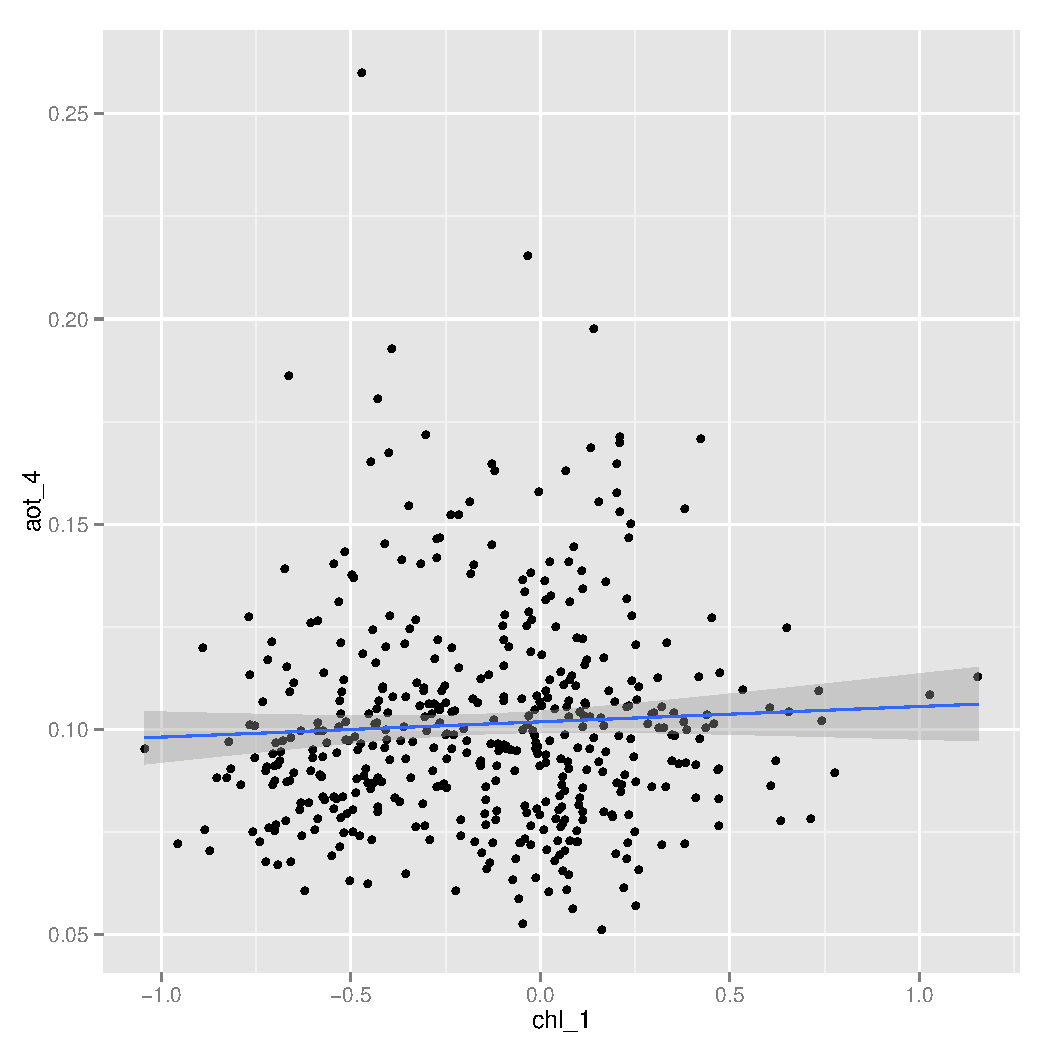
\includegraphics[width=\maxwidth]{figure/unnamed-chunk-22-1} 
\begin{kframe}\begin{alltt}
\hlcom{## Correlation coefficient}
\hlkwd{cor}\hlstd{(df}\hlopt{$}\hlstd{chl_1, df}\hlopt{$}\hlstd{aot_4,} \hlkwc{use}\hlstd{=}\hlstr{'complete.obs'}\hlstd{)}
\end{alltt}
\begin{verbatim}
## [1] 0.05161445
\end{verbatim}
\begin{alltt}
\hlkwd{ccf}\hlstd{(df}\hlopt{$}\hlstd{chl_1, df}\hlopt{$}\hlstd{aot_4,} \hlkwc{na.action}\hlstd{=na.pass)}
\end{alltt}
\end{kframe}
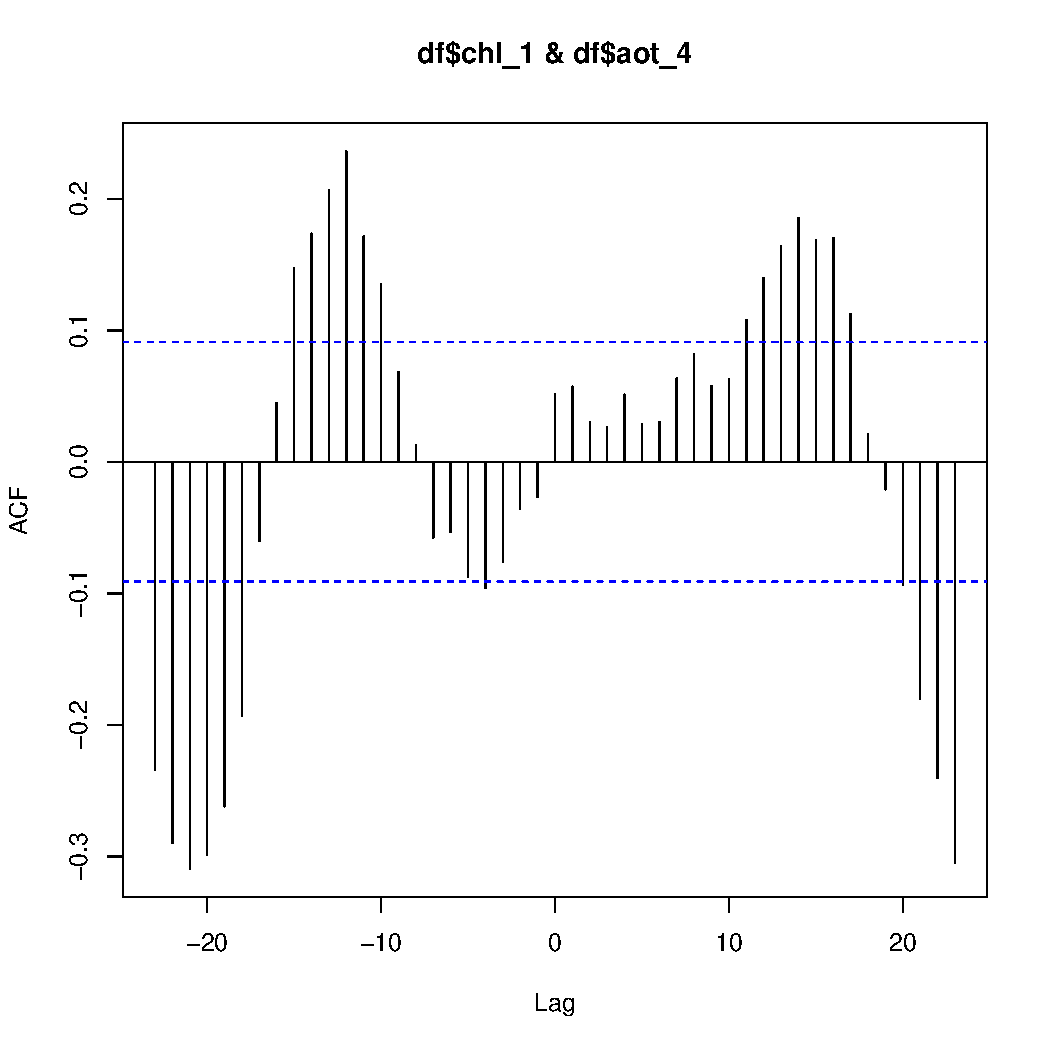
\includegraphics[width=\maxwidth]{figure/unnamed-chunk-22-2} 

\end{knitrout}

\subsection{Chlorophyll and Rain}

\begin{knitrout}
\definecolor{shadecolor}{rgb}{0.969, 0.969, 0.969}\color{fgcolor}\begin{kframe}
\begin{alltt}
\hlkwd{qplot}\hlstd{(chl_1,} \hlkwd{log}\hlstd{(rain_1),} \hlkwc{data}\hlstd{=df,} \hlkwc{geom}\hlstd{=}\hlkwd{c}\hlstd{(}\hlstr{'point'}\hlstd{,} \hlstr{'smooth'}\hlstd{),} \hlkwc{method}\hlstd{=}\hlstr{'lm'}\hlstd{,} \hlkwc{formula}\hlstd{=y}\hlopt{~}\hlstd{x)}
\end{alltt}
\end{kframe}
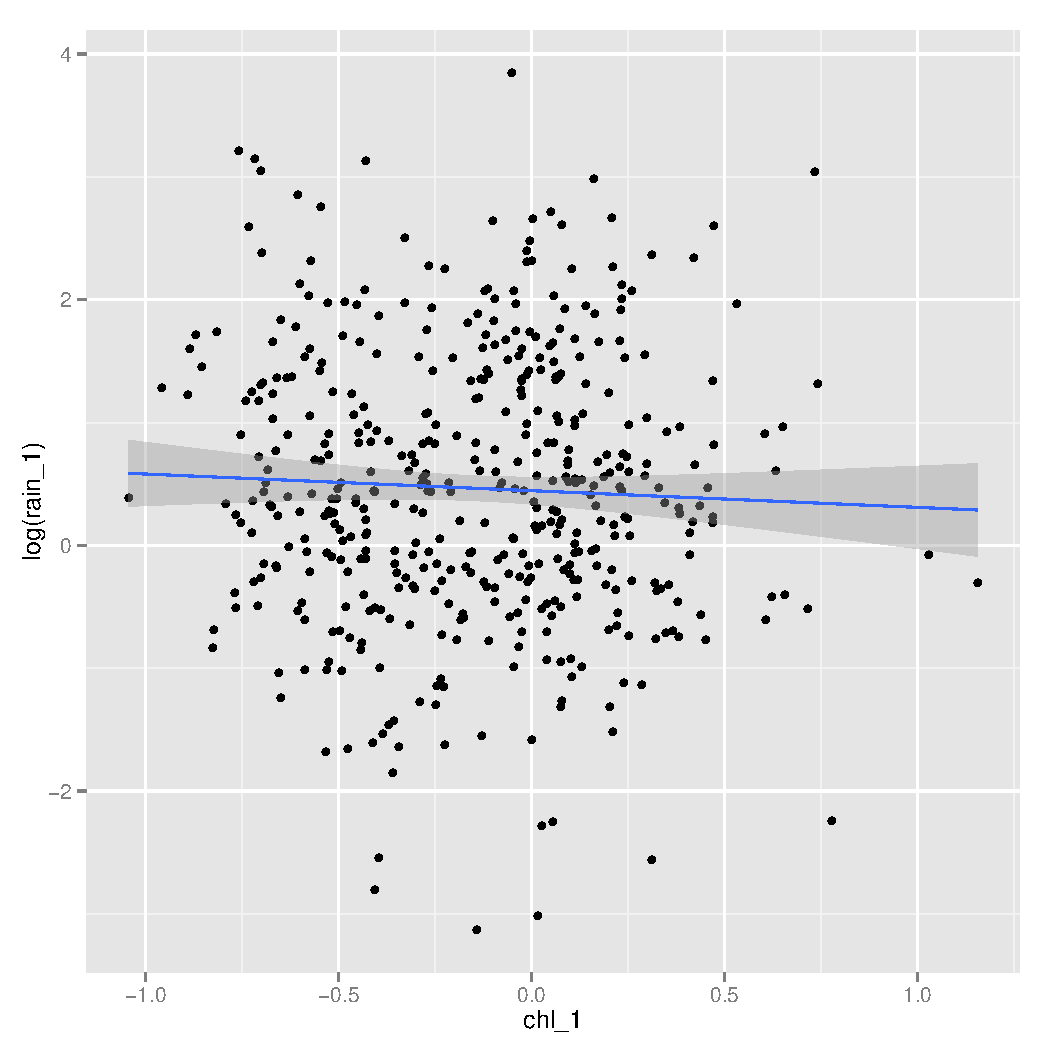
\includegraphics[width=\maxwidth]{figure/unnamed-chunk-23-1} 
\begin{kframe}\begin{alltt}
\hlcom{## Correlation coefficient}
\hlkwd{cor}\hlstd{(df}\hlopt{$}\hlstd{chl_1,} \hlkwd{log}\hlstd{(df}\hlopt{$}\hlstd{rain_1),} \hlkwc{use}\hlstd{=}\hlstr{'complete.obs'}\hlstd{)}
\end{alltt}
\begin{verbatim}
## [1] -0.04447456
\end{verbatim}
\begin{alltt}
\hlkwd{ccf}\hlstd{(df}\hlopt{$}\hlstd{chl_1,} \hlkwd{log}\hlstd{(df}\hlopt{$}\hlstd{rain_1),} \hlkwc{na.action}\hlstd{=na.pass)}
\end{alltt}
\end{kframe}
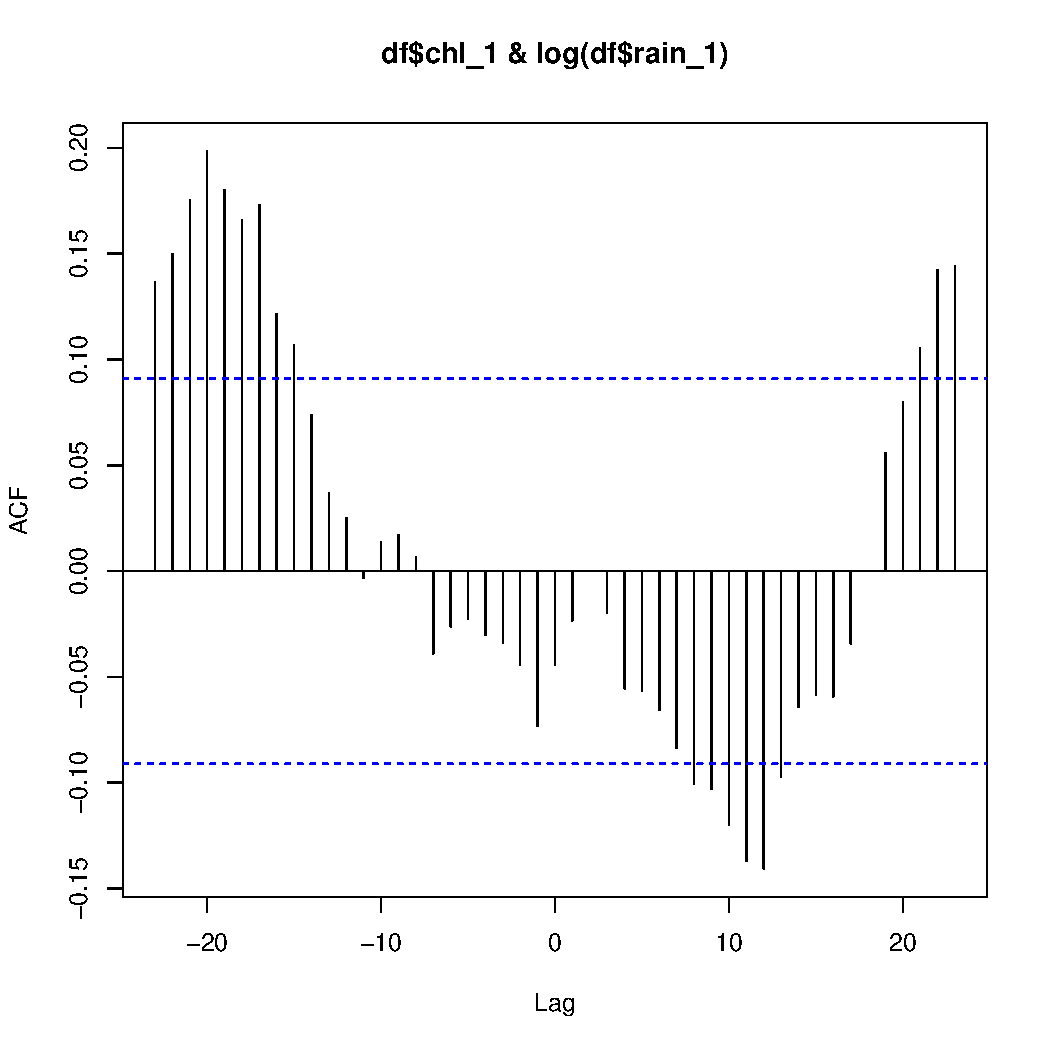
\includegraphics[width=\maxwidth]{figure/unnamed-chunk-23-2} 

\end{knitrout}

\begin{knitrout}
\definecolor{shadecolor}{rgb}{0.969, 0.969, 0.969}\color{fgcolor}\begin{kframe}
\begin{alltt}
\hlkwd{qplot}\hlstd{(chl_1,} \hlkwd{log}\hlstd{(rain_2),} \hlkwc{data}\hlstd{=df,} \hlkwc{geom}\hlstd{=}\hlkwd{c}\hlstd{(}\hlstr{'point'}\hlstd{,} \hlstr{'smooth'}\hlstd{),} \hlkwc{method}\hlstd{=}\hlstr{'lm'}\hlstd{,} \hlkwc{formula}\hlstd{=y}\hlopt{~}\hlstd{x)}
\end{alltt}
\end{kframe}
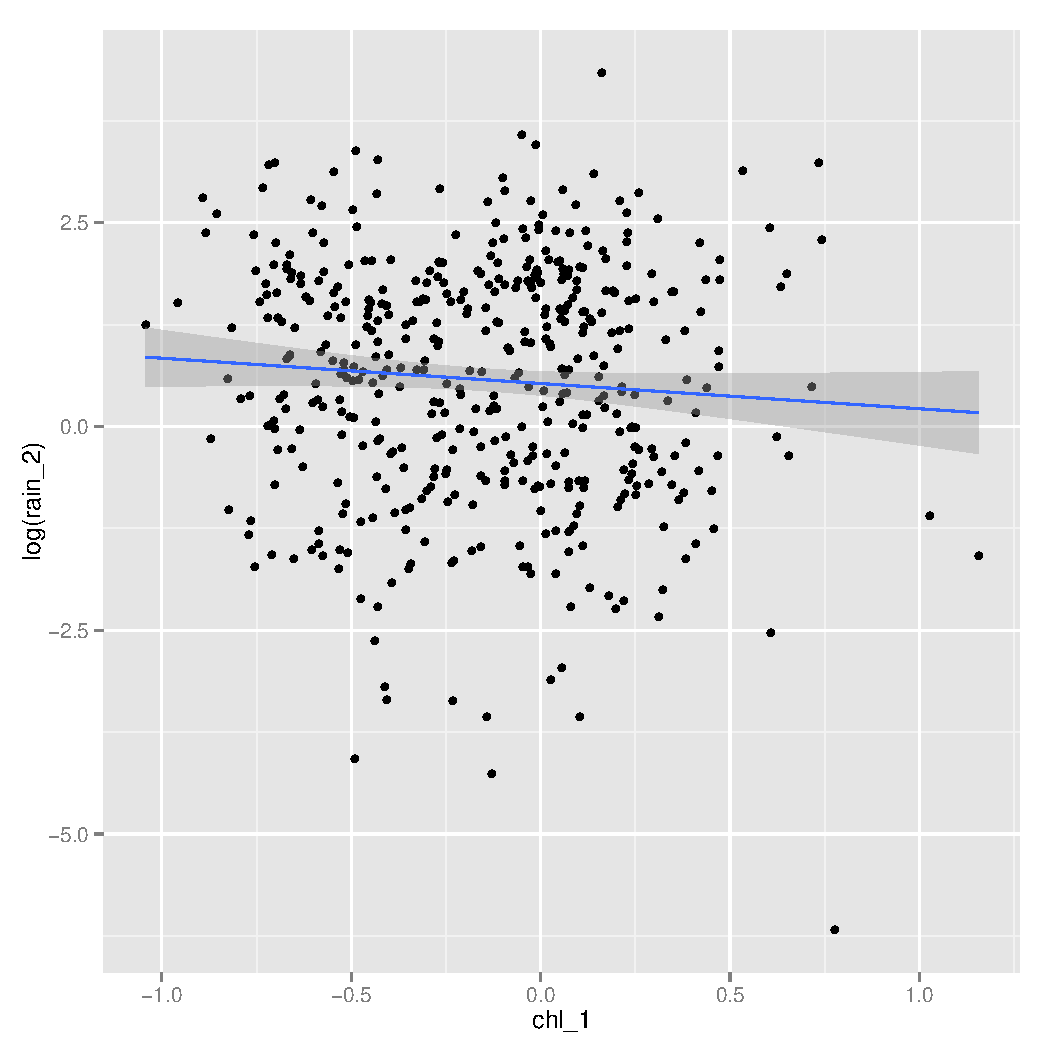
\includegraphics[width=\maxwidth]{figure/unnamed-chunk-24-1} 
\begin{kframe}\begin{alltt}
\hlcom{## Correlation coefficient}
\hlkwd{cor}\hlstd{(df}\hlopt{$}\hlstd{chl_1,} \hlkwd{log}\hlstd{(df}\hlopt{$}\hlstd{rain_2),} \hlkwc{use}\hlstd{=}\hlstr{'complete.obs'}\hlstd{)}
\end{alltt}
\begin{verbatim}
## [1] -0.07603666
\end{verbatim}
\begin{alltt}
\hlkwd{ccf}\hlstd{(df}\hlopt{$}\hlstd{chl_1,} \hlkwd{log}\hlstd{(df}\hlopt{$}\hlstd{rain_2),} \hlkwc{na.action}\hlstd{=na.pass)}
\end{alltt}
\end{kframe}
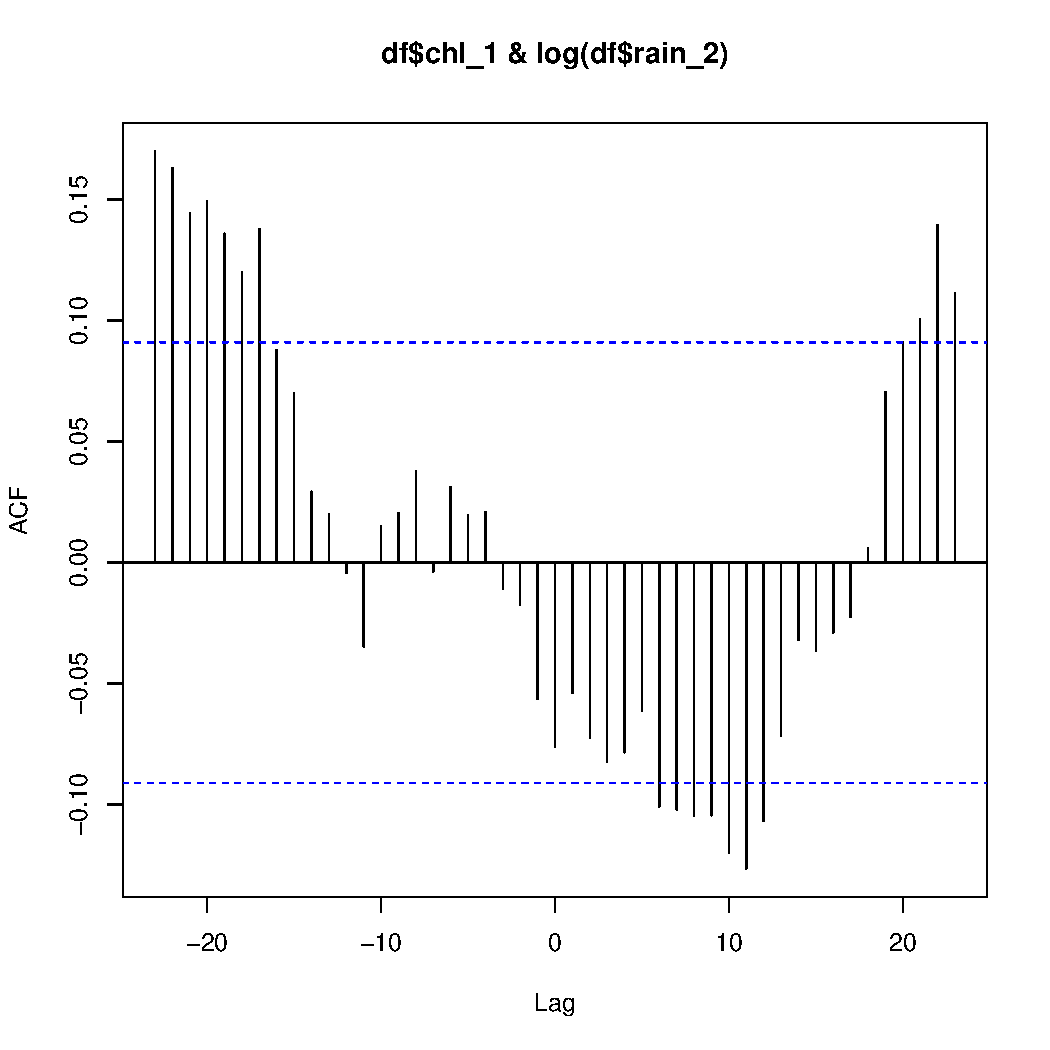
\includegraphics[width=\maxwidth]{figure/unnamed-chunk-24-2} 

\end{knitrout}

\begin{knitrout}
\definecolor{shadecolor}{rgb}{0.969, 0.969, 0.969}\color{fgcolor}\begin{kframe}
\begin{alltt}
\hlkwd{qplot}\hlstd{(chl_1,} \hlkwd{log}\hlstd{(rain_3),} \hlkwc{data}\hlstd{=df,} \hlkwc{geom}\hlstd{=}\hlkwd{c}\hlstd{(}\hlstr{'point'}\hlstd{,} \hlstr{'smooth'}\hlstd{),} \hlkwc{method}\hlstd{=}\hlstr{'lm'}\hlstd{,} \hlkwc{formula}\hlstd{=y}\hlopt{~}\hlstd{x)}
\end{alltt}
\end{kframe}
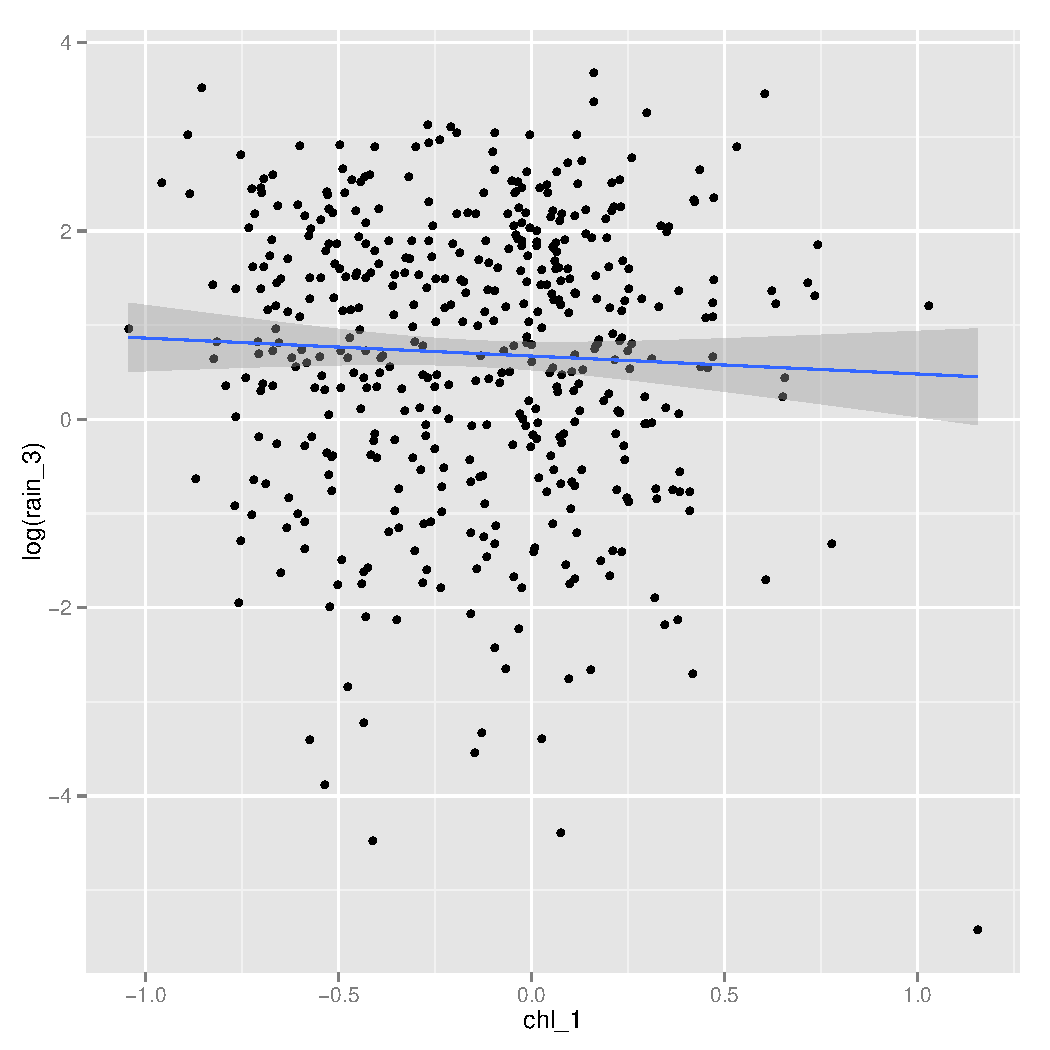
\includegraphics[width=\maxwidth]{figure/unnamed-chunk-25-1} 
\begin{kframe}\begin{alltt}
\hlcom{## Correlation coefficient}
\hlkwd{cor}\hlstd{(df}\hlopt{$}\hlstd{chl_1,} \hlkwd{log}\hlstd{(df}\hlopt{$}\hlstd{rain_3),} \hlkwc{use}\hlstd{=}\hlstr{'complete.obs'}\hlstd{)}
\end{alltt}
\begin{verbatim}
## [1] -0.046129
\end{verbatim}
\begin{alltt}
\hlkwd{ccf}\hlstd{(df}\hlopt{$}\hlstd{chl_1,} \hlkwd{log}\hlstd{(df}\hlopt{$}\hlstd{rain_3),} \hlkwc{na.action}\hlstd{=na.pass)}
\end{alltt}
\end{kframe}
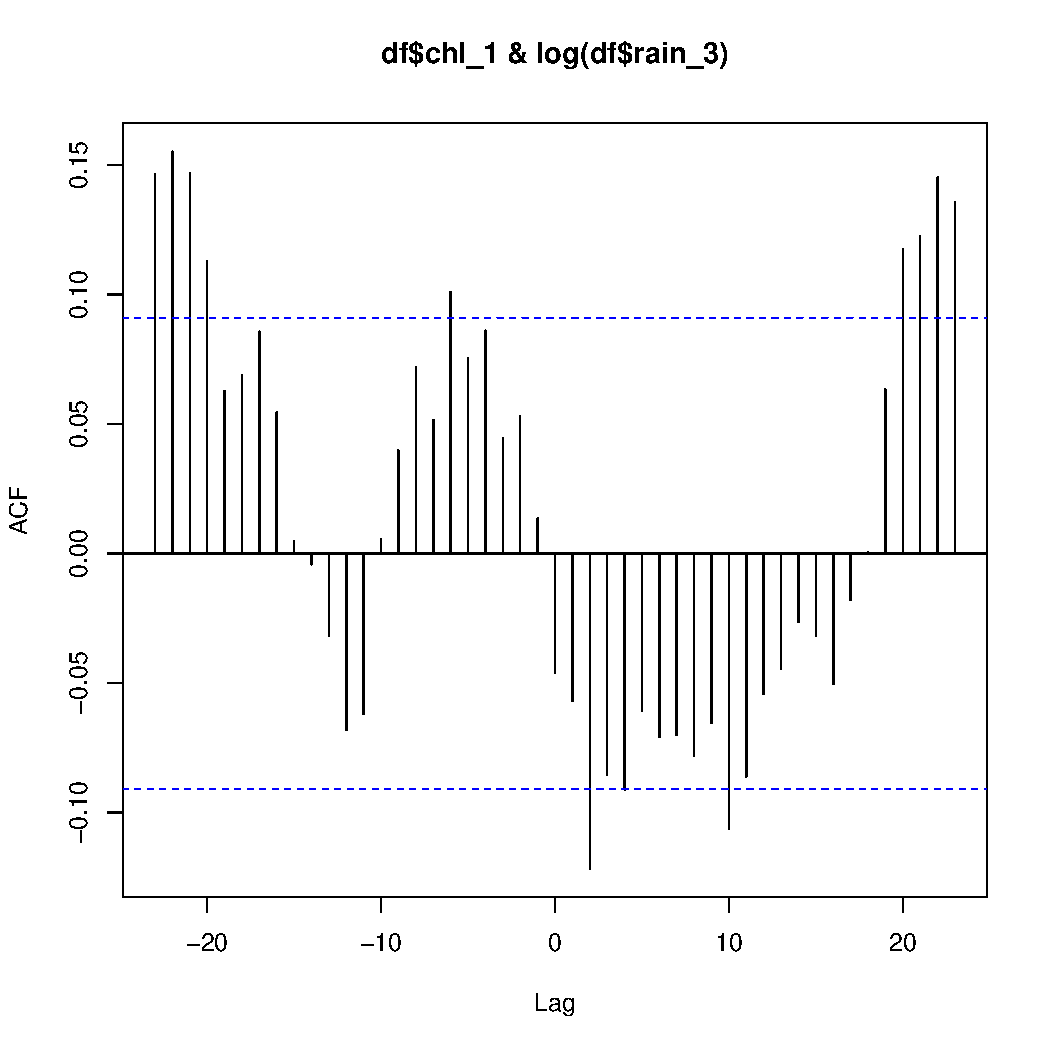
\includegraphics[width=\maxwidth]{figure/unnamed-chunk-25-2} 

\end{knitrout}

\begin{knitrout}
\definecolor{shadecolor}{rgb}{0.969, 0.969, 0.969}\color{fgcolor}\begin{kframe}
\begin{alltt}
\hlkwd{qplot}\hlstd{(chl_1,} \hlkwd{log}\hlstd{(rain_4),} \hlkwc{data}\hlstd{=df,} \hlkwc{geom}\hlstd{=}\hlkwd{c}\hlstd{(}\hlstr{'point'}\hlstd{,} \hlstr{'smooth'}\hlstd{),} \hlkwc{method}\hlstd{=}\hlstr{'lm'}\hlstd{,} \hlkwc{formula}\hlstd{=y}\hlopt{~}\hlstd{x)}
\end{alltt}
\end{kframe}
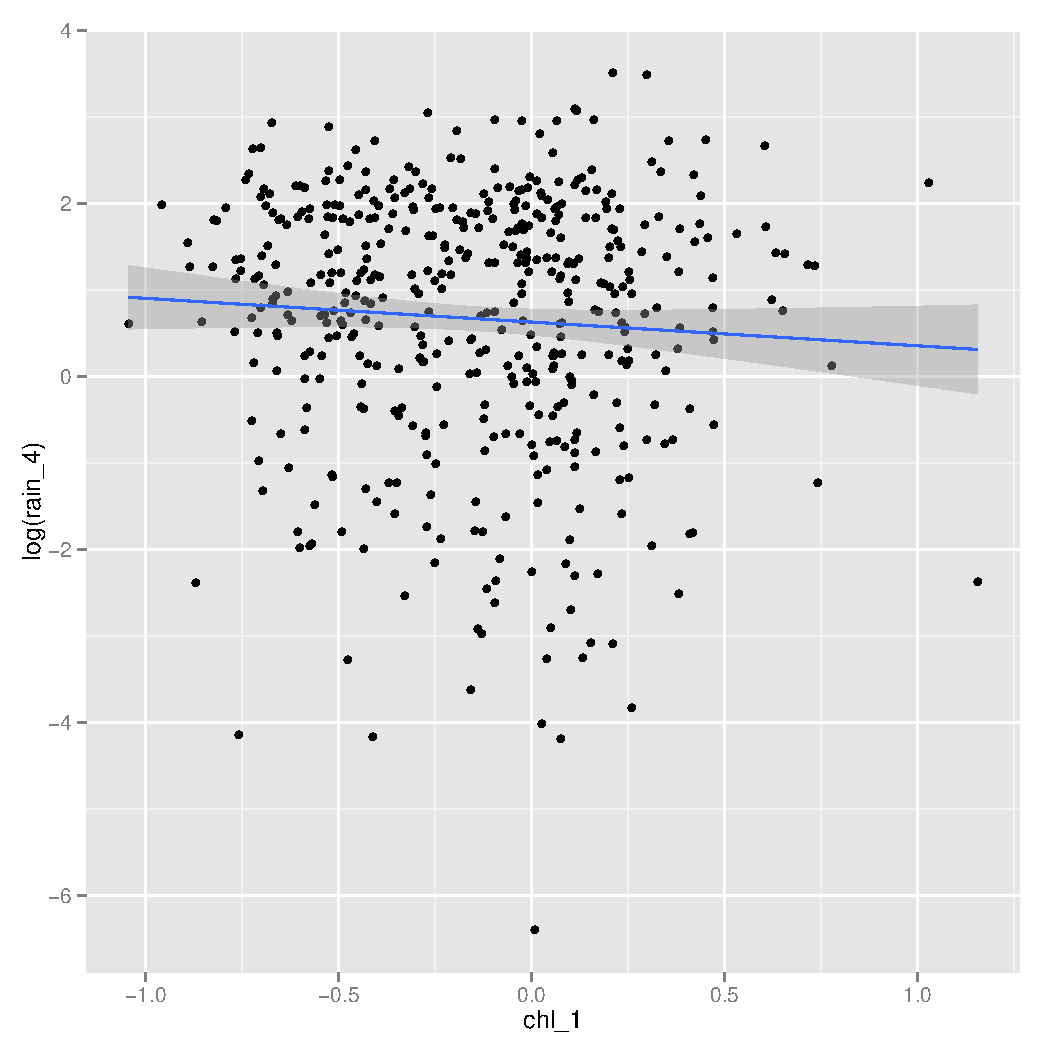
\includegraphics[width=\maxwidth]{figure/unnamed-chunk-26-1} 
\begin{kframe}\begin{alltt}
\hlcom{## Correlation coefficient}
\hlkwd{cor}\hlstd{(df}\hlopt{$}\hlstd{chl_1,} \hlkwd{log}\hlstd{(df}\hlopt{$}\hlstd{rain_4),} \hlkwc{use}\hlstd{=}\hlstr{'complete.obs'}\hlstd{)}
\end{alltt}
\begin{verbatim}
## [1] -0.0657788
\end{verbatim}
\begin{alltt}
\hlkwd{ccf}\hlstd{(df}\hlopt{$}\hlstd{chl_1,} \hlkwd{log}\hlstd{(df}\hlopt{$}\hlstd{rain_4),} \hlkwc{na.action}\hlstd{=na.pass)}
\end{alltt}
\end{kframe}
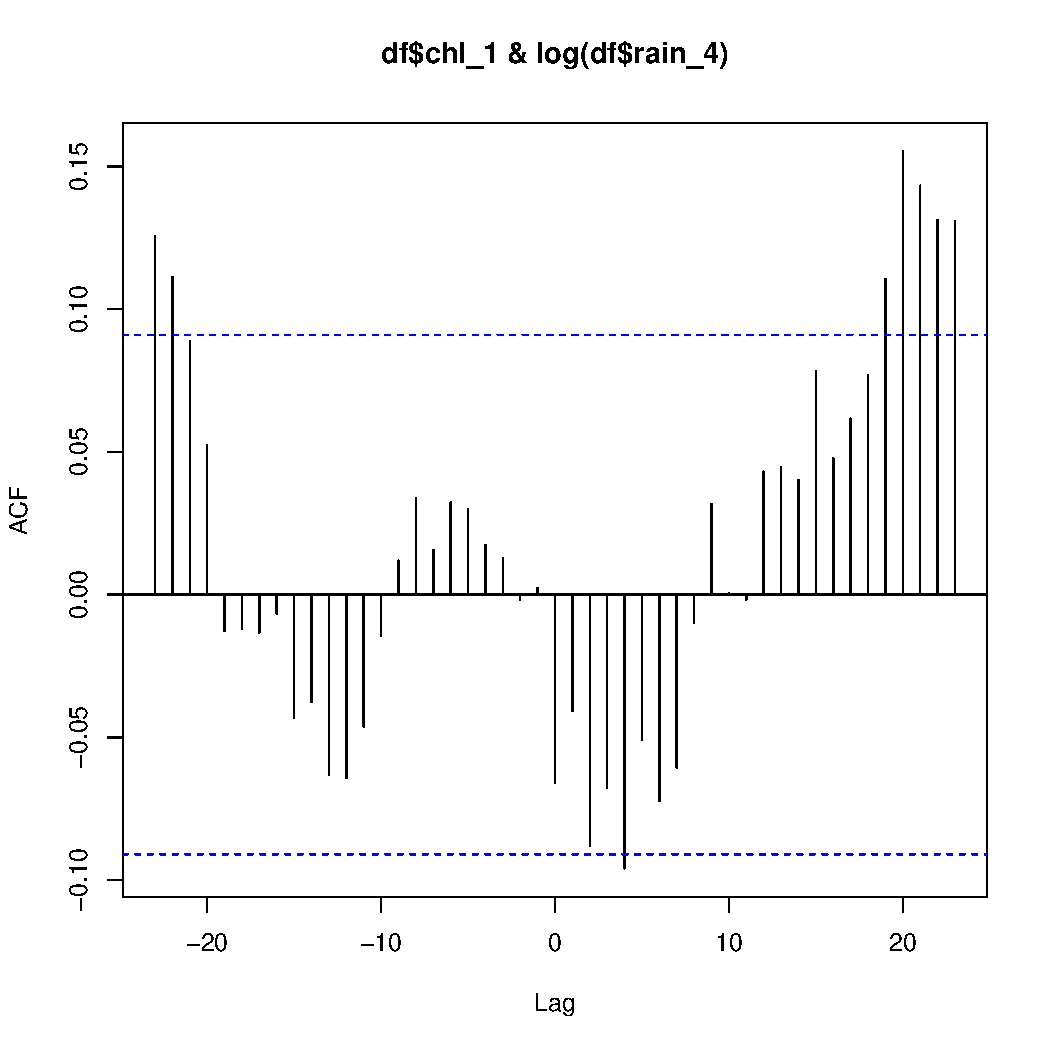
\includegraphics[width=\maxwidth]{figure/unnamed-chunk-26-2} 

\end{knitrout}

\subsection{Chlorophyll and wind}

\begin{knitrout}
\definecolor{shadecolor}{rgb}{0.969, 0.969, 0.969}\color{fgcolor}\begin{kframe}
\begin{alltt}
\hlkwd{qplot}\hlstd{(chl_1, wndpwr_1,} \hlkwc{data}\hlstd{=df,} \hlkwc{geom}\hlstd{=}\hlkwd{c}\hlstd{(}\hlstr{'point'}\hlstd{,} \hlstr{'smooth'}\hlstd{),} \hlkwc{method}\hlstd{=}\hlstr{'lm'}\hlstd{,} \hlkwc{formula}\hlstd{=y}\hlopt{~}\hlstd{x)}
\end{alltt}
\end{kframe}
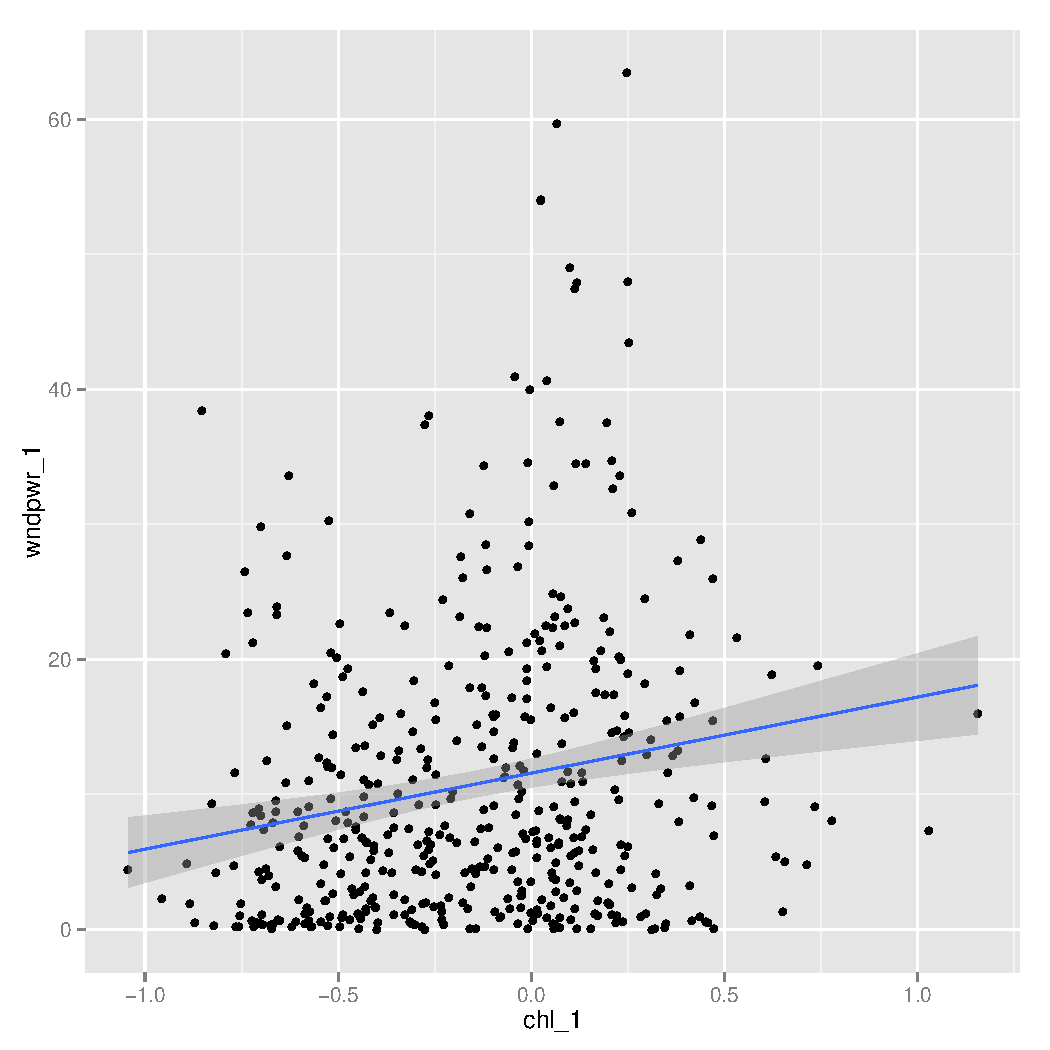
\includegraphics[width=\maxwidth]{figure/unnamed-chunk-27-1} 
\begin{kframe}\begin{alltt}
\hlcom{## Correlation coefficient}
\hlkwd{cor}\hlstd{(df}\hlopt{$}\hlstd{chl_1, df}\hlopt{$}\hlstd{wndpwr_1,} \hlkwc{use}\hlstd{=}\hlstr{'complete.obs'}\hlstd{)}
\end{alltt}
\begin{verbatim}
## [1] 0.1892394
\end{verbatim}
\begin{alltt}
\hlkwd{ccf}\hlstd{(df}\hlopt{$}\hlstd{chl_1, df}\hlopt{$}\hlstd{wndpwr_1,} \hlkwc{na.action}\hlstd{=na.pass)}
\end{alltt}
\end{kframe}
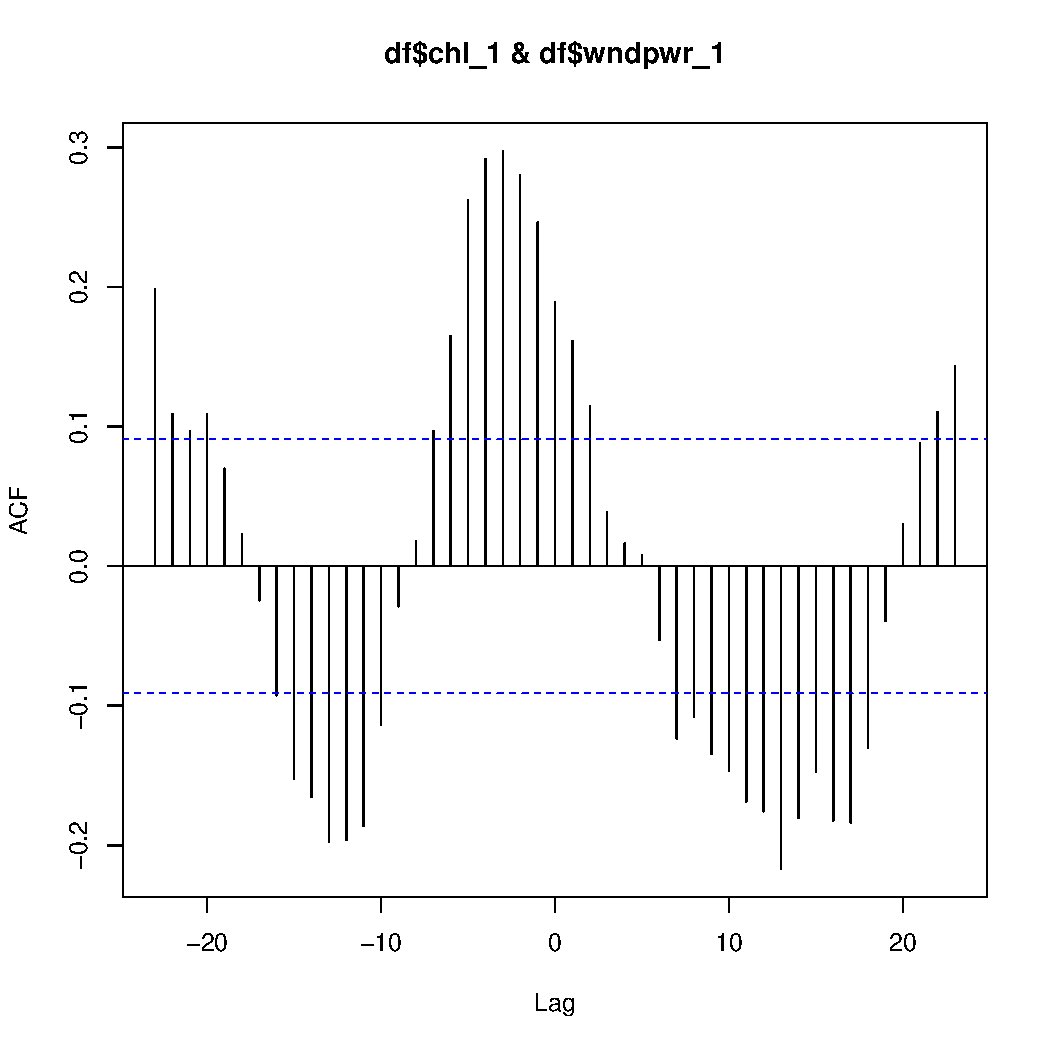
\includegraphics[width=\maxwidth]{figure/unnamed-chunk-27-2} 

\end{knitrout}

\begin{knitrout}
\definecolor{shadecolor}{rgb}{0.969, 0.969, 0.969}\color{fgcolor}\begin{kframe}
\begin{alltt}
\hlkwd{qplot}\hlstd{(chl_1, wndpwr_2,} \hlkwc{data}\hlstd{=df,} \hlkwc{geom}\hlstd{=}\hlkwd{c}\hlstd{(}\hlstr{'point'}\hlstd{,} \hlstr{'smooth'}\hlstd{),} \hlkwc{method}\hlstd{=}\hlstr{'lm'}\hlstd{,} \hlkwc{formula}\hlstd{=y}\hlopt{~}\hlstd{x)}
\end{alltt}
\end{kframe}
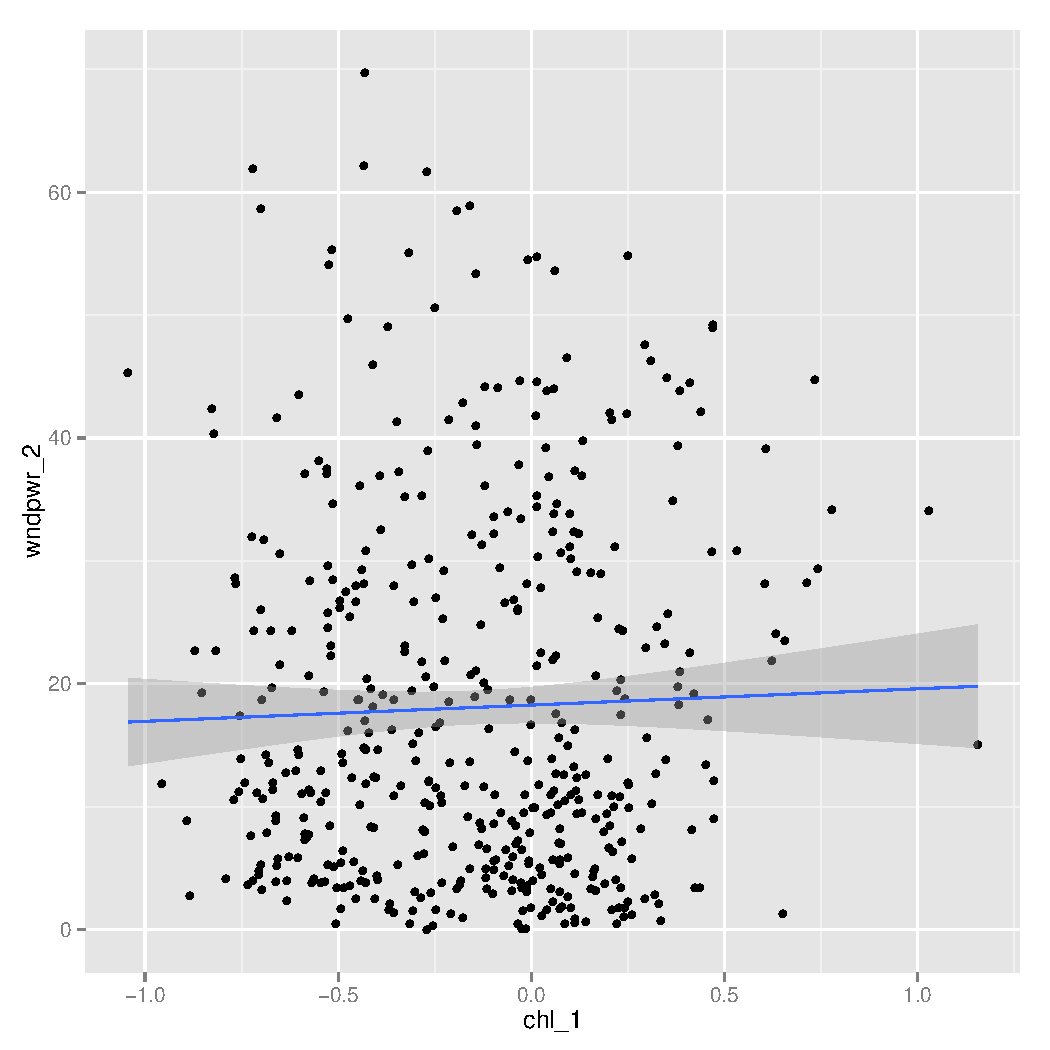
\includegraphics[width=\maxwidth]{figure/unnamed-chunk-28-1} 
\begin{kframe}\begin{alltt}
\hlcom{## Correlation coefficient}
\hlkwd{cor}\hlstd{(df}\hlopt{$}\hlstd{chl_1, df}\hlopt{$}\hlstd{wndpwr_2,} \hlkwc{use}\hlstd{=}\hlstr{'complete.obs'}\hlstd{)}
\end{alltt}
\begin{verbatim}
## [1] 0.03268013
\end{verbatim}
\begin{alltt}
\hlkwd{ccf}\hlstd{(df}\hlopt{$}\hlstd{chl_1, df}\hlopt{$}\hlstd{wndpwr_2,} \hlkwc{na.action}\hlstd{=na.pass)}
\end{alltt}
\end{kframe}
\includegraphics[width=\maxwidth]{figure/unnamed-chunk-28-2} 

\end{knitrout}

\begin{knitrout}
\definecolor{shadecolor}{rgb}{0.969, 0.969, 0.969}\color{fgcolor}\begin{kframe}
\begin{alltt}
\hlkwd{qplot}\hlstd{(chl_1, wndpwr_3,} \hlkwc{data}\hlstd{=df,} \hlkwc{geom}\hlstd{=}\hlkwd{c}\hlstd{(}\hlstr{'point'}\hlstd{,} \hlstr{'smooth'}\hlstd{),} \hlkwc{method}\hlstd{=}\hlstr{'lm'}\hlstd{,} \hlkwc{formula}\hlstd{=y}\hlopt{~}\hlstd{x)}
\end{alltt}
\end{kframe}
\includegraphics[width=\maxwidth]{figure/unnamed-chunk-29-1} 
\begin{kframe}\begin{alltt}
\hlcom{## Correlation coefficient}
\hlkwd{cor}\hlstd{(df}\hlopt{$}\hlstd{chl_1, df}\hlopt{$}\hlstd{wndpwr_3,} \hlkwc{use}\hlstd{=}\hlstr{'complete.obs'}\hlstd{)}
\end{alltt}
\begin{verbatim}
## [1] 0.03603483
\end{verbatim}
\begin{alltt}
\hlkwd{ccf}\hlstd{(df}\hlopt{$}\hlstd{chl_1, df}\hlopt{$}\hlstd{wndpwr_3,} \hlkwc{na.action}\hlstd{=na.pass)}
\end{alltt}
\end{kframe}
\includegraphics[width=\maxwidth]{figure/unnamed-chunk-29-2} 

\end{knitrout}

\begin{knitrout}
\definecolor{shadecolor}{rgb}{0.969, 0.969, 0.969}\color{fgcolor}\begin{kframe}
\begin{alltt}
\hlkwd{qplot}\hlstd{(chl_1, wndpwr_4,} \hlkwc{data}\hlstd{=df,} \hlkwc{geom}\hlstd{=}\hlkwd{c}\hlstd{(}\hlstr{'point'}\hlstd{,} \hlstr{'smooth'}\hlstd{),} \hlkwc{method}\hlstd{=}\hlstr{'lm'}\hlstd{,} \hlkwc{formula}\hlstd{=y}\hlopt{~}\hlstd{x)}
\end{alltt}
\end{kframe}
\includegraphics[width=\maxwidth]{figure/unnamed-chunk-30-1} 
\begin{kframe}\begin{alltt}
\hlcom{## Correlation coefficient}
\hlkwd{cor}\hlstd{(df}\hlopt{$}\hlstd{chl_1, df}\hlopt{$}\hlstd{wndpwr_4,} \hlkwc{use}\hlstd{=}\hlstr{'complete.obs'}\hlstd{)}
\end{alltt}
\begin{verbatim}
## [1] 0.06274202
\end{verbatim}
\begin{alltt}
\hlkwd{ccf}\hlstd{(df}\hlopt{$}\hlstd{chl_1, df}\hlopt{$}\hlstd{wndpwr_4,} \hlkwc{na.action}\hlstd{=na.pass)}
\end{alltt}
\end{kframe}
\includegraphics[width=\maxwidth]{figure/unnamed-chunk-30-2} 

\end{knitrout}

\subsection{Chlorophyll and indices}

\begin{knitrout}
\definecolor{shadecolor}{rgb}{0.969, 0.969, 0.969}\color{fgcolor}\begin{kframe}
\begin{alltt}
\hlkwd{qplot}\hlstd{(chl_1, imi,} \hlkwc{data}\hlstd{=df,} \hlkwc{geom}\hlstd{=}\hlkwd{c}\hlstd{(}\hlstr{'point'}\hlstd{,} \hlstr{'smooth'}\hlstd{))}\hlcom{#, method='lm', formula=y~x)}
\end{alltt}


{\ttfamily\noindent\itshape\color{messagecolor}{\#\# geom\_smooth: method="{}auto"{} and size of largest group is <1000, so using loess. Use 'method = x' to change the smoothing method.}}\end{kframe}
\includegraphics[width=\maxwidth]{figure/unnamed-chunk-31-1} 
\begin{kframe}\begin{alltt}
\hlcom{## Correlation coefficient}
\hlkwd{cor}\hlstd{(df}\hlopt{$}\hlstd{chl_1, df}\hlopt{$}\hlstd{imi,} \hlkwc{use}\hlstd{=}\hlstr{'complete.obs'}\hlstd{)}
\end{alltt}
\begin{verbatim}
## [1] 0.2074861
\end{verbatim}
\begin{alltt}
\hlkwd{ccf}\hlstd{(df}\hlopt{$}\hlstd{chl_1, df}\hlopt{$}\hlstd{imi,} \hlkwc{na.action}\hlstd{=na.pass)}
\end{alltt}
\end{kframe}
\includegraphics[width=\maxwidth]{figure/unnamed-chunk-31-2} 

\end{knitrout}

\begin{knitrout}
\definecolor{shadecolor}{rgb}{0.969, 0.969, 0.969}\color{fgcolor}\begin{kframe}
\begin{alltt}
\hlkwd{qplot}\hlstd{(chl_1, nao,} \hlkwc{data}\hlstd{=df,} \hlkwc{geom}\hlstd{=}\hlkwd{c}\hlstd{(}\hlstr{'point'}\hlstd{,} \hlstr{'smooth'}\hlstd{),} \hlkwc{method}\hlstd{=}\hlstr{'lm'}\hlstd{,} \hlkwc{formula}\hlstd{=y}\hlopt{~}\hlstd{x)}
\end{alltt}
\end{kframe}
\includegraphics[width=\maxwidth]{figure/unnamed-chunk-32-1} 
\begin{kframe}\begin{alltt}
\hlcom{## Correlation coefficient}
\hlkwd{cor}\hlstd{(df}\hlopt{$}\hlstd{chl_1, df}\hlopt{$}\hlstd{nao,} \hlkwc{use}\hlstd{=}\hlstr{'complete.obs'}\hlstd{)}
\end{alltt}
\begin{verbatim}
## [1] 0.004341686
\end{verbatim}
\begin{alltt}
\hlkwd{ccf}\hlstd{(df}\hlopt{$}\hlstd{chl_1, df}\hlopt{$}\hlstd{nao,} \hlkwc{na.action}\hlstd{=na.pass)}
\end{alltt}
\end{kframe}
\includegraphics[width=\maxwidth]{figure/unnamed-chunk-32-2} 

\end{knitrout}

\begin{knitrout}
\definecolor{shadecolor}{rgb}{0.969, 0.969, 0.969}\color{fgcolor}\begin{kframe}
\begin{alltt}
\hlkwd{qplot}\hlstd{(chl_1, soi,} \hlkwc{data}\hlstd{=df,} \hlkwc{geom}\hlstd{=}\hlkwd{c}\hlstd{(}\hlstr{'point'}\hlstd{,} \hlstr{'smooth'}\hlstd{),} \hlkwc{method}\hlstd{=}\hlstr{'lm'}\hlstd{,} \hlkwc{formula}\hlstd{=y}\hlopt{~}\hlstd{x)}
\end{alltt}
\end{kframe}
\includegraphics[width=\maxwidth]{figure/unnamed-chunk-33-1} 
\begin{kframe}\begin{alltt}
\hlcom{## Correlation coefficient}
\hlkwd{cor}\hlstd{(df}\hlopt{$}\hlstd{chl_1, df}\hlopt{$}\hlstd{soi,} \hlkwc{use}\hlstd{=}\hlstr{'complete.obs'}\hlstd{)}
\end{alltt}
\begin{verbatim}
## [1] -0.07367003
\end{verbatim}
\begin{alltt}
\hlkwd{ccf}\hlstd{(df}\hlopt{$}\hlstd{chl_1, df}\hlopt{$}\hlstd{soi,} \hlkwc{na.action}\hlstd{=na.pass)}
\end{alltt}
\end{kframe}
\includegraphics[width=\maxwidth]{figure/unnamed-chunk-33-2} 

\end{knitrout}

\section{Region 2 (Southern Central Red Sea)}

\subsection{Correlation with other variables}

The Correlation level between CHL in the southern central cluster
and other environmental variable.
The most important are in the order: CHL (clusters 3 and 4), PAR, wind, 
IMI, SSH, rain.

\begin{knitrout}
\definecolor{shadecolor}{rgb}{0.969, 0.969, 0.969}\color{fgcolor}\begin{kframe}
\begin{alltt}
\hlstd{tot_cor} \hlkwb{<-} \hlkwd{cor}\hlstd{(df[,}\hlopt{-}\hlkwd{c}\hlstd{(}\hlnum{1}\hlstd{,}\hlnum{2}\hlstd{,}\hlnum{3}\hlstd{)],} \hlkwc{use}\hlstd{=}\hlstr{'complete'}\hlstd{)}
\hlstd{chl_cor} \hlkwb{<-} \hlstd{tot_cor[}\hlstr{'chl_2'}\hlstd{,]}
\hlstd{chl_cor} \hlkwb{<-} \hlkwd{sort}\hlstd{(chl_cor,} \hlkwc{decreasing}\hlstd{=}\hlnum{TRUE}\hlstd{)}
\hlkwd{names}\hlstd{(chl_cor)} \hlkwb{<-} \hlkwd{factor}\hlstd{(}\hlkwd{names}\hlstd{(chl_cor),} \hlkwc{levels}\hlstd{=}\hlkwd{names}\hlstd{(chl_cor))}
\hlkwd{qplot}\hlstd{(}\hlkwd{factor}\hlstd{(}\hlkwd{names}\hlstd{(chl_cor),} \hlkwc{levels}\hlstd{=}\hlkwd{names}\hlstd{(chl_cor)), chl_cor,} \hlkwc{geom}\hlstd{=}\hlstr{'bar'}\hlstd{,} \hlkwc{stat}\hlstd{=}\hlstr{'identity'}\hlstd{)} \hlopt{+} \hlkwd{theme}\hlstd{(}\hlkwc{axis.text.x} \hlstd{=} \hlkwd{element_text}\hlstd{(}\hlkwc{angle} \hlstd{=} \hlnum{90}\hlstd{,} \hlkwc{hjust} \hlstd{=} \hlnum{1}\hlstd{))}
\end{alltt}


{\ttfamily\noindent\color{warningcolor}{\#\# Warning: Stacking not well defined when ymin != 0}}\end{kframe}
\includegraphics[width=\maxwidth]{figure/unnamed-chunk-34-1} 

\end{knitrout}

\section{Region 3 (Northern Central Red Sea)}

\subsection{Correlation with other variables}

The Correlation level between CHL in the northern central cluster
and other environmental variable.
The most important are in the order: CHL (clusters 2 and 4), wind, PAR,
IMI, SSH, rain.

\begin{knitrout}
\definecolor{shadecolor}{rgb}{0.969, 0.969, 0.969}\color{fgcolor}\begin{kframe}
\begin{alltt}
\hlstd{tot_cor} \hlkwb{<-} \hlkwd{cor}\hlstd{(df[,}\hlopt{-}\hlkwd{c}\hlstd{(}\hlnum{1}\hlstd{,}\hlnum{2}\hlstd{,}\hlnum{3}\hlstd{)],} \hlkwc{use}\hlstd{=}\hlstr{'complete'}\hlstd{)}
\hlstd{chl_cor} \hlkwb{<-} \hlstd{tot_cor[}\hlstr{'chl_3'}\hlstd{,]}
\hlstd{chl_cor} \hlkwb{<-} \hlkwd{sort}\hlstd{(chl_cor,} \hlkwc{decreasing}\hlstd{=}\hlnum{TRUE}\hlstd{)}
\hlkwd{names}\hlstd{(chl_cor)} \hlkwb{<-} \hlkwd{factor}\hlstd{(}\hlkwd{names}\hlstd{(chl_cor),} \hlkwc{levels}\hlstd{=}\hlkwd{names}\hlstd{(chl_cor))}
\hlkwd{qplot}\hlstd{(}\hlkwd{factor}\hlstd{(}\hlkwd{names}\hlstd{(chl_cor),} \hlkwc{levels}\hlstd{=}\hlkwd{names}\hlstd{(chl_cor)), chl_cor,} \hlkwc{geom}\hlstd{=}\hlstr{'bar'}\hlstd{,} \hlkwc{stat}\hlstd{=}\hlstr{'identity'}\hlstd{)} \hlopt{+} \hlkwd{theme}\hlstd{(}\hlkwc{axis.text.x} \hlstd{=} \hlkwd{element_text}\hlstd{(}\hlkwc{angle} \hlstd{=} \hlnum{90}\hlstd{,} \hlkwc{hjust} \hlstd{=} \hlnum{1}\hlstd{))}
\end{alltt}


{\ttfamily\noindent\color{warningcolor}{\#\# Warning: Stacking not well defined when ymin != 0}}\end{kframe}
\includegraphics[width=\maxwidth]{figure/unnamed-chunk-35-1} 

\end{knitrout}

\section{Region 4 (Northern Red Sea)}

\subsection{Correlation with other variables}

The Correlation level between CHL in the northern cluster
and other environmental variable.
The most important are in the order: CHL (clusters 3 and 2), IMI, Wind, PAR, SSH.

\begin{knitrout}
\definecolor{shadecolor}{rgb}{0.969, 0.969, 0.969}\color{fgcolor}\begin{kframe}
\begin{alltt}
\hlstd{tot_cor} \hlkwb{<-} \hlkwd{cor}\hlstd{(df[,}\hlopt{-}\hlkwd{c}\hlstd{(}\hlnum{1}\hlstd{,}\hlnum{2}\hlstd{,}\hlnum{3}\hlstd{)],} \hlkwc{use}\hlstd{=}\hlstr{'complete'}\hlstd{)}
\hlstd{chl_cor} \hlkwb{<-} \hlstd{tot_cor[}\hlstr{'chl_4'}\hlstd{,]}
\hlstd{chl_cor} \hlkwb{<-} \hlkwd{sort}\hlstd{(chl_cor,} \hlkwc{decreasing}\hlstd{=}\hlnum{TRUE}\hlstd{)}
\hlkwd{names}\hlstd{(chl_cor)} \hlkwb{<-} \hlkwd{factor}\hlstd{(}\hlkwd{names}\hlstd{(chl_cor),} \hlkwc{levels}\hlstd{=}\hlkwd{names}\hlstd{(chl_cor))}
\hlkwd{qplot}\hlstd{(}\hlkwd{factor}\hlstd{(}\hlkwd{names}\hlstd{(chl_cor),} \hlkwc{levels}\hlstd{=}\hlkwd{names}\hlstd{(chl_cor)), chl_cor,} \hlkwc{geom}\hlstd{=}\hlstr{'bar'}\hlstd{,} \hlkwc{stat}\hlstd{=}\hlstr{'identity'}\hlstd{)} \hlopt{+} \hlkwd{theme}\hlstd{(}\hlkwc{axis.text.x} \hlstd{=} \hlkwd{element_text}\hlstd{(}\hlkwc{angle} \hlstd{=} \hlnum{90}\hlstd{,} \hlkwc{hjust} \hlstd{=} \hlnum{1}\hlstd{))}
\end{alltt}


{\ttfamily\noindent\color{warningcolor}{\#\# Warning: Stacking not well defined when ymin != 0}}\end{kframe}
\includegraphics[width=\maxwidth]{figure/unnamed-chunk-36-1} 

\end{knitrout}

\end{document}
